%% This is the main file and you use this file to organize your assignment.

\documentclass[a4paper]{article}	  
\usepackage{geometry} 	   % Choose your margin here. 
\usepackage{amsmath}
\usepackage{amssymb}
\usepackage{parskip}
\usepackage{graphicx}
\usepackage{caption}
\usepackage{float}
\usepackage{todonotes}
\usepackage{caption}
\usepackage{subcaption}
\usepackage{hyperref}
\usepackage{cleveref}
\usepackage{svg}
\DeclareMathOperator*{\argmax}{arg\,max}
\DeclareMathOperator*{\argmin}{arg\,min}
\newcommand{\norm}[1]{\left\lVert#1\right\rVert}

\newcommand{\figref}[1]{\figurename~\ref{#1}}

\let\endtitlepage\relax	% Begin the text immidiately after the title page. Optional
\setlength{\parindent}{0cm}				% Start paragraph without indent. Optional

\begin{document}

\begin{titlepage}
\begin{center}
\Large Semesteroppgave\\
\vspace{10pt}
\Large CrazyFlie trilateration network\\
\vspace{10pt}
\large Magnus Berdal
\end{center}
\end{titlepage}
\clearpage
\tableofcontents
% Use "\include" instead of "\input" if you want the section to start on a new page.
\section{Introduction}

A first responder (FR) is a person who is among those responsible for going immediately to the scene of an accident or emergency to provide assistance \cite{FR}.
They will typically be employed by the emergency services such as the police, fire department or health services, and take it upon themselves to secure the health of people, property and the enivornment.
Often times this includes sacrificing their own safety in order to secure that of others. The the need for quick action gives them no other choice.

Search-and-rescue personell in particular expose themselves to dangerous environments. Burning buildings, collapsed or flooded caves etc. are just some examples of the rapid-changing
hazardeous evironments in which FRs can find themselves. Often times they enter without any knowledge of what is waiting for them on the other side. Imagine a burning building. The local fire department has just arrived. There is no time to 
spare, so the first firefighters enter to save the lives of those inside before the floor plan is inspected. It might not even be valid as the roaring fire continues to eat up the walls and support beams for the roof. Still the firefighters enter in order to rescue those inside.
If something is to happen to the entering firefighters there is no way to locate them, and the ones entering to save them still don't know what is waiting for them inside.

Advancements in technology can be used to limit the dangers to which FRs expose themselves. With the increasing performance and decreasing cost of mobile robots, and the ability to outfit them with whatever equipment one might think of, it is relevant to think of how 
this might be used to the advantage of first responders. Using disposable robots for tasks such as mapping the environment could drastically improve the safety of FRs. In the example stated above, mobile robots could be dispatched into the burning house
and continuously feed the firedighters with a real time map of the environment. Robots could also enter the building to set up an ad-hoc network \cite{GAVHALE2016477} used for locating FRs inside GNSS denied environments, or supply information about events happening, such as changes in the environment or the
presence of poisenous gasses etc.

The challenge in creating such ad-hoc networks lay in enabling the robots to quickly set up the network as desired without supervision. This is the matter that will be studied in this report.
\section{Background}\label[sec]{background}
\subsection{Potential, Limitations and Progress of the MAV}
Micro Areal Vehicles (MAVs) have great potential in contributing to indoor search-and-rescue missions. Their small size and weight
make them easy to transport and allows for rapid field deployment. Furthermore they are agile, allowing them to operate in 
complex environments and access hard-to-get-to places.

Limitations of current technologies, prohibiting the existence of fully autonomous MAVs, are examined in \cite{MAV_enabling}. They define the following
requirements for a fully autonomous MAV:
\begin{itemize}
  \item Inference: The ability to infer situational awareness from sensory measurements.
  \item Reasoning: The ability to define a mission based on abstract human-defined goals.
  \item Unsupervised learning: The ability to adapt and learn its own control strategies without human supervision.
\end{itemize}
Due to the constraints on the size of MAVs, the existence of fully autonomous MAVs is mainly dependent on the existence of 
small and efficient hardware components such as power supplies, sensors and processors allowing them to quickly process incoming data and convert this information into actions.
The authors of \cite{MAV_enabling} conclude that as of March 2017 no fully autonomous MAV system exist.

Although a fully autonomous MAV system is yet to be realized, the advancement in transistor density shown in \figref{trans_density}, and the continuously diminishing price of microprocessors continue to
allow for faster, and thus more complex, on-board computations. This allows for enhanced autonomous capabilities of the aircraft \cite{MAV_enabling}. Increased onboard computation power enables the aircraft to perform 
computations of increased complexity locally without the aid of other computation units or human interference, while conforming with real-time constraints.
\begin{figure}[H]
  \centering
  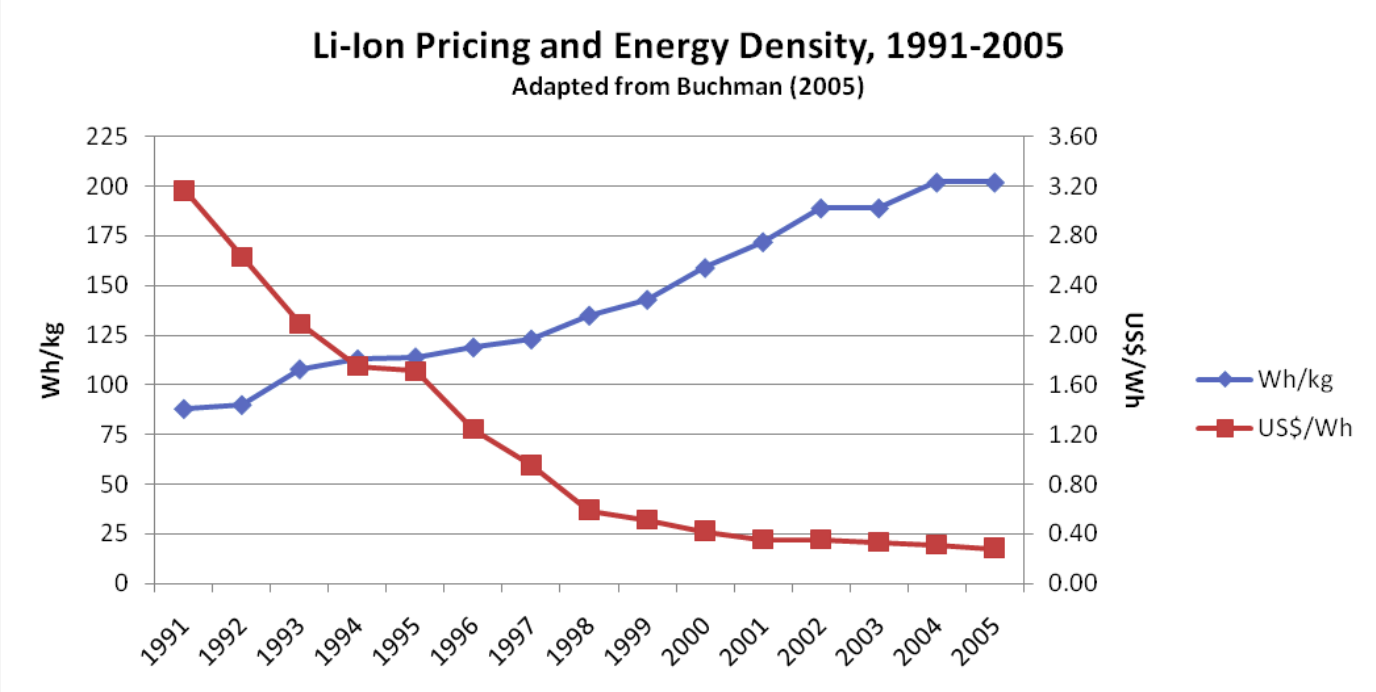
\includegraphics[width=.85\textwidth]{figs/lion-price.png}
  \caption{Evolution of energy density and cost of Lithium-ion batteries. Source: \cite{lion}.}
  \label[fig]{lion_price}
\end{figure}
\clearpage
\begin{figure}[h]
  \centering
  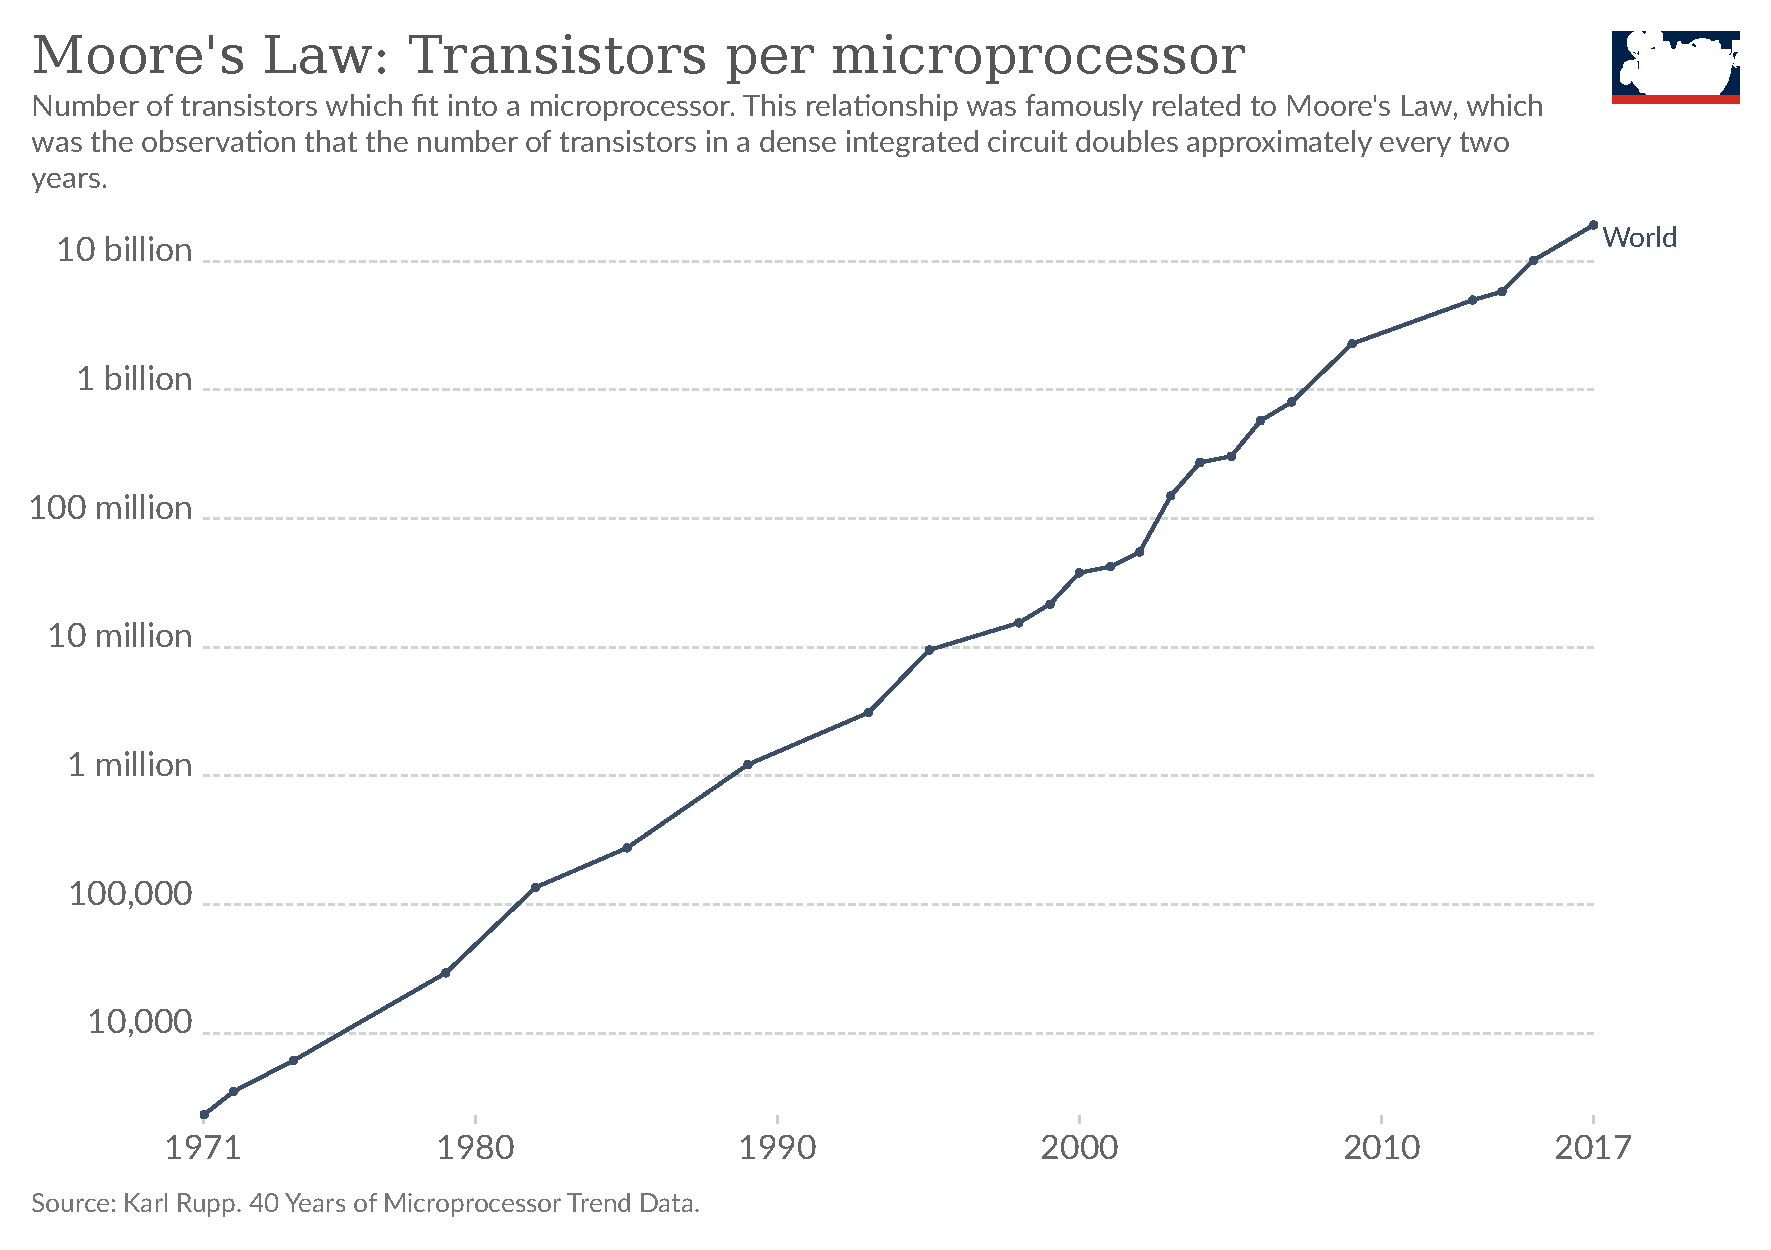
\includegraphics[width=.75\textwidth]{figs/transistors-per-microprocessor.pdf}
  \caption{Evolution of the number of transistors per microprocessor.}
  \label[fig]{trans_density}
\end{figure}

Most MAVs utilize electrical propulsion systems. This is due to the ability to miniaturize electrical propulsion systems for MAV applications with minimal loss of efficiency. Furthermore electrical propulsion systems have faster response time than combustion based systems \cite{MAV_enabling}. Energy is typically stored on
LiPo\footnote{Lithium-ion polymer} batteries. \figref{lion_price} shows how the energy density and price of Lithium-ion batteries have evolved over the last decades. As the energy density of Lithium-ion batteries already have and is projected to continue to increase \cite{lion_density}, this will allow 
for fitting more power consuming equipment on the MAVs, and increasing their endurance. Thus enabling MAVs to take on more complex and long lasting missions, resulting in increased autonomy.

Not only hardware components have made leaps over the last decades. The advancement in autonomy of MAV systems through the creation of efficient and lightweight software has been a field of great scientific interest.
The Robotics \& Perception Group at the University of Z\"urich have performed excessive research into the field of visual-inertial based real-time navigation and mapping
by MAVs in GNSS denied environments \cite{svo2, svo1}. The goal of which is enabling MAVs to localize themselves in and map unknown environments without external aid.

In \cite{svo2} a fast and robust visual-odometry algorithm (SVO) is presented. The method is faster than previously presented methods, and is therefore especially useful 
for MAV operations as it should be able to run on a onboard computer with limited processing power. It is concluded that the method is especially useful for state estimation onboard MAVs as the algorithm runs
at a high enough rate to provide accurate state estimates. Furthermore, the use of depth-filters yields an accurate map of the environment with few outliers.

In \cite{svo1} Scaramuzza et al. present a system for autonomous mapping of unknown indoor and outdoor environments performed by a single MAV using SVO. The MAV is supplied with 
a trajectory it is to follow, and using only on-board processing and sensing, follows said trajectory and provides at the same time a real-time map of the environment.

Developments such as those in \cite{svo2} and \cite{svo1} have increased the autonomous capabilities of MAVs, and as time passes more efficient software solutions will continue to do so.

\subsection{The Deployment Problem \& Blanket Coverage}
Multi-agent distributed control is the task of making a set of agents work together to fulfill some collective goal, and doing so 
with only local information. One such task is studied in this report, self-deployment: Make a swarm of robots "[...] deploy 
themselves in an environment without central coordination"\cite{BAYINDIR2016292}. A subcategory of the deployment problem is referred to 
in literature as the blanket coverage problem. In \cite{BAYINDIR2016292} the blanket coverage problem is defined as the task of finding a static 
configuration of agents such that a cost function is maximized over an area.

Cassandras and Zhong present in \cite{cassandras} a distributed method for a multi-agent blanket coverage.
They approach the blanket coverage problem using a probability based objective function. With their approach the 
goal of the set of agents is maximizing the joint detection probability of randomly occurring events in the environment. 
They also present an algorithm that preserves connectivity of the network of agents. They conclude that using their method, the swarm of agents reach a configuration corresponding to a 
local maxima of the joint detection probability function. Furthermore they find that when connectivity preservation is imposed, the swarm settles at a configuration in which the joint detection probability is
smaller than when connectivity of the network is not taken into account.

In \cite{sun2014escaping} Cassandras and Zhong "[...] address the problem of multiple local optima
commonly arising in optimization problems for multi-agent systems[...]". Utilizing the same probability based objective function as in \cite{cassandras}, boosting functions are applied to encourage agents to explore poorly
covered regions of the area and escape local optima. Three families of boosting functions are defined and tested through simulations. It is shown that the objective value post boosting is no worse than before.

Howard et.al. present in \cite{pot_field} another approach to the blanket coverage problem: virtual potential fields. It is assumed that 
agents are able to determine the range and bearing to both nearby agents and obstacles. Drawing inspiration from 
electrostatic fields, agents are seen on as point charges who exert repulsive forces on one another, causing them to spread. Furthermore
obstacles also exert forces on the agents so that agents do not collide with obstacles in the environment. They show through simulations
that the potential field approach can be used to deploy multi-agent networks for the means of blanket coverage, and conclude that area
coverage emerges from a combination of "[...] purely local rules"\cite{pot_field}.

\clearpage
\subsection{Multilateration}\label[ssec]{trilat}
Multilateration is the process of determining the positions of unknown points in space by measurements of distances from known points \cite{trilat_website}. In order
to perform this task in two-dimensional space, at least three known points are needed.

Given $n\geq 3$ beacons located at positions $\mathbf{x}_{a}\in\mathbb{R}^{2},\; 0\leq a<n$ where not all points
lie on a single line, the location 
of an entity, denoted by $\mathbf{y}\in\mathbb{R}^{2}$, can be determined as follows:
\begin{enumerate}
  \item The entity broadcasts signal and starts a timer at $t_{0}$.
  \item Beacons at $\mathbf{x}_{a},\; 0\leq a<n$ receive broadcasted signal and immediately responds with a packet containing $\mathbf{x}_{a}$.
  \item When receiving the packet from beacon at $\mathbf{x}_{a}$, the entity stores the time of reception in a variable $t_{1, a}$.
  \item When at least 3 beacons have responded, the entity calculates the distance
  from itself to beacon at $\mathbf{x}_{a}$: $d_{a} = \frac{1}{2}s(t_{1, a} - t_{0})$, where $s$ is the propagation speed of the signal. The factor $\frac{1}{2}$ is due to the signal traveling
  two times the distance between the entity and the beacon placed at $\mathbf{x}_{a}$ (the ping travels from the entity to the agent, and the packet
  sent by the agent travels back again).
  \item Based on the distances, $d_{a}$, and the positions of the beacons the entity can
  determine its position by calculating the point where circles centered at $\mathbf{x}_{a}$ with radii $d_{a}$ intersect.
\end{enumerate}
If sufficiently many beacons respond an ML (Maximum Likelihood) estimator of the position of the entity can be computed \cite{10.1145/381677.381693}.
Defining the error function:\begin{equation}
  e_{a}(\mathbf{y}) = s(t_{1, a} - t_{0, a}) - \norm{\mathbf{x}_{a} - \mathbf{y}} = d_{a} - \norm{\mathbf{x}_{a} - \mathbf{y}}
\end{equation}
An estimate of the position of the entity is obtained by solving:
\begin{equation}
  \hat{\mathbf{y}} = \argmin_{\mathbf{y}} \mathbf{E}^{T}\mathbf{E},\quad\mathbf{E} = \begin{bmatrix}
    e_{0}(\mathbf{y})\\
    \vdots\\
    e_{n-1}(\mathbf{y})
  \end{bmatrix}
\end{equation}
The position estimation error is affected by the measurement errors, by the geometry relating sensors and target, and by the estimation algorithm \cite{trilat_error}.
As the pings travel at large velocities (the speed of light) the resolution of the internal clock of the parties involved set a bound on the accuracy of the estimated position.
As was found in \cite{CRB_multilat}, multilateration of the unknown position of an entity is most accurate when the entity is placed nearby or within the convex hull of the beacons. Hence spreading
the beacons is desirable in order to obtain accurate position estimates.
\figref{trilat_example} shows how the position of an entity can be determined from the known positions of 3 agents.
\begin{figure}[H]
  \centering
  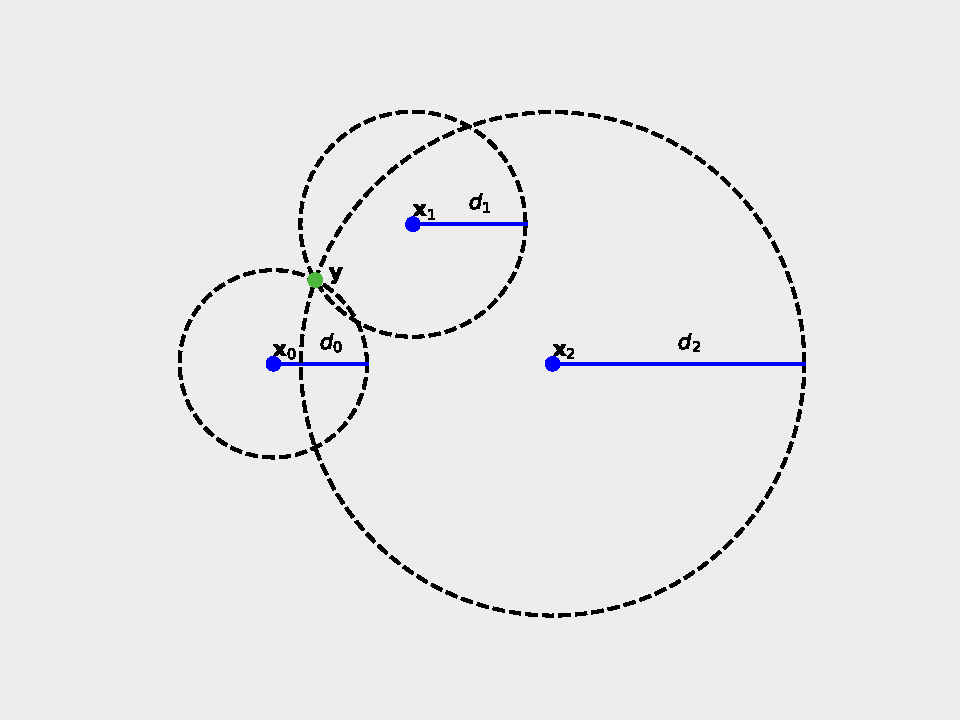
\includegraphics[width=.7\textwidth]{figs/trilateration_example.pdf}
  \caption{Position, $\mathbf{y}$, of entity determined by multilateration using known positions of $3$ beacons placed at $\mathbf{x}_{0}$, $\mathbf{x}_{1}$ and $\mathbf{x}_{2}$. The distances
  $d_{0}$, $d_{1}$ and $d_{2}$ are determined by sending pings between the entity at $\mathbf{y}$ and the beacons. The point $\mathbf{y}$ lies at the intersection of the circles placed at 
  $\mathbf{x}_{a}$ with radius $d_{a}$, $a = 0, 1, 2$.}
  \label[fig]{trilat_example}
\end{figure}
\section{Notation}
\begin{itemize}
  \item $\Omega$: Mission space.
  \item $\mathcal{O}$: Set of obstacles inside the mission space.
  \item $\mathcal{F}$: Feasible space.
  \item $\mathbf{x}_{a}$: Position of agent $a$.
  \item $r_{a}$: Maximum communication range of agent $a$.
  \item $\hat{p}(\mathbf{x}_{a}, \mathbf{y})$: Probability of agent $a$ being able to communicate with entity at position $\mathbf{y}$.
  \item $V_{a}$: Visible set of agent $a$.
  \item $U_{a}$: Invisible set of agent $a$.
  \item $\mathbf{X}_{\mathcal{S}}$: Positions of all agents in the swarm $\mathcal{S}$.
  \item $\Phi^{n}(\mathbf{X_{\mathcal{S}}}, \mathbf{y})$: Probability of $n$ members in the swarm $\mathcal{S}$ being able to communicate with entity at position $\mathbf{y}$.
  \item $\Phi^{n^{+}}(\mathbf{X_{\mathcal{S}}}, \mathbf{y})$: Probability of $n$ or more members in the swarm $\mathcal{S}$ being able to communicate with entity at position $\mathbf{y}$.
\end{itemize}

\subsection{Mathematical operators}
\begin{itemize}
  \item For a set $\mathcal{S}$ defined by $\mathcal{S} = \{s_{0}\hdots s_{N-1}\},\;N<\infty$ we define:
  \begin{itemize}
    \item $|\mathcal{S}| = N$: The size of $\mathcal{S}$.
    \item $\mathrm{Comb}(\mathcal{S}, n) = \{\mathcal{A}: \mathcal{A}\subseteq\mathcal{S}, |\mathcal{A}|=n\}$: the set of all subsets of $\mathcal{S}$ of size $n$.
  \end{itemize}
  \item For a set $\mathcal{S}$ of points $\mathbf{x}\in\mathbb{R}^{N}$ defined by $\mathcal{S} = \{\mathbf{x}\in\mathbb{R}^{N}: f(\mathbf{x})\leq\mathbf{0}\}$ we define:
  \begin{itemize}
    \item $\delta\mathcal{S} = \{\mathbf{x}\in\mathbb{R}^{N}: f(\mathbf{x}) = \mathbf{0}\}$: The boundary of $\mathcal{S}$.
    \item $\mathrm{int}(\mathcal{S}) = \{\mathbf{x}\in\mathbb{R}^{N}: f(\mathbf{x}) < \mathbf{0}\}$: The interior of $\mathcal{S}$.
    \item $A(\mathcal{S})$: The area of the space bounded by $\delta\mathcal{S}$.
  \end{itemize}
\end{itemize}
\section{System Description}

\subsection{Notation}
A set $\mathcal{S}$ of points $\mathbf{x}\in\mathbb{R}^{2}$ is defined by it's boundary, $\delta\mathcal{S}$, 
and it's interior, $\mathrm{int}(\mathcal{S})$. The number of elements in a set $\mathcal{S}$ is denoted as $|\mathcal{S}|$.\newline
The $Comb(\cdot)$ operator takes as arguments a set $\mathcal{S}$ and an integer $n$ and returns all subset of $\mathcal{S}$ of lenght $n$:
\begin{equation}
  Comb(\mathcal{S}, n) = \{\mathcal{A}: \mathcal{A}\subseteq\mathcal{S}, |\mathcal{A}|=n\}
\end{equation}

\subsection{Feasible space}
As in \cite{sun2014escaping}, a \textit{mission space}, $\Omega$, is defined as a simple polygon 
\cite{weissteinsimplepolygon}.
Within the mission space there exists $N_{o}\geq 0$ obstacles, each one of which is defined as a simple polygon.
The set of all obstacles, $\mathcal{O}$, is defined according to \eqref{obstacle_set_def}.
\begin{equation}\label[eq]{obstacle_set_def}
  \mathcal{O} = \begin{cases}
    \{o_{0}\hdots o_{N_{o}-1}\} &, N_{o} > 0\\
    \emptyset &, N_{o} = 0\\
  \end{cases}
\end{equation}
The obstacles in $\mathcal{O}$ constrains the movement of entities within the mission space, as it is not possible to
penetrate the boundary of an obstacle. Due to this, once an entity is inside $\Omega$, it is constrained to be positioned within
$\Omega$ and outside $\mathrm{int}(o)\;\forall\;o\in\mathcal{O}$. From this we define the \textit{feasible space}, $\mathcal{F}$, as
all points where it is possible to place an entity:
\begin{equation}\label[eq]{feasible_space_def}
  \mathcal{F} = \{\mathbf{y}\in\mathbb{R}^{2}: \mathbf{y}\in\Omega,\;\mathbf{y}\notin\mathrm{int}(o)\;\forall\;o\in\mathcal{O}\} = \Omega\setminus\bigcup_{o\in\mathcal{O}}\mathrm{int}(o)
\end{equation}

\subsection{Agent}
An \textit{agent}, denoted by an integer $a$, is defined by its position $\mathbf{x}_{a}\in\mathbb{R}^{2}$ and 
its maximum range of communication $r_{a}$. From this we define the communication disk of agent $a$:
\begin{equation}
  D_{a} = \{\mathbf{y}\in\mathbb{R}^{2}: \norm{\mathbf{x}_{a} - \mathbf{y}}\leq r_{a}\}
\end{equation}
Assuming line-of-sight (LoS) communication, meaning an agent cannot communicate with an entity if there is an obstacle or a mission space wall between them, we define the \textit{visible set} of agent 
$a$:
\begin{equation}\label[eq]{visible_set_def}
  V(\mathbf{x}_{a}, r_{a}) = \{\mathbf{y}\in\mathbb{R}^{2}:\mathbf{y}\in D_{a}, \lambda\mathbf{y} + (1-\lambda)\mathbf{x}_{a}\in\mathcal{F}\;\forall\;0\leq\lambda\leq 1\}
\end{equation}
The counterpart to the visible set, called the invisible set of agent $a$, is simply defined as:
\begin{equation}
  V_{c}(\mathbf{x}_{a}, r_{a}) = \mathcal{F}\setminus V(\mathbf{x}_{a}, r_{a})
\end{equation}
An example of the visible set for an agent is show in \figref{vis_set_example}.

The probability of an agent $a$ being able to communicate with another entity positioned at a point $\mathbf{y}$, from now on called
the local probability of agent $a$, is defined according to:
\todo{Find notation for $\mathbb{R}^{5}$ with non-negative values in last dimension}
\begin{equation}\label[eq]{local_prob}
  \hat{p}:(\mathbb{R}^{2}, \mathbb{R}^{2}, \mathbb{R}^{+})\rightarrow [0, 1]\quad\hat{p}(\mathbf{x}_{a}, r_{a}, \mathbf{y}) = \begin{cases}
    p(\norm{\mathbf{x}_{a}-\mathbf{y}})>0 &, \mathbf{y}\in V(\mathbf{x}_{a}, r_{a})\\
    0 &, \mathbf{y}\in V_{c}(\mathbf{x}_{a}, r_{a})
  \end{cases}
\end{equation}
\begin{figure}[H]
  \centering
  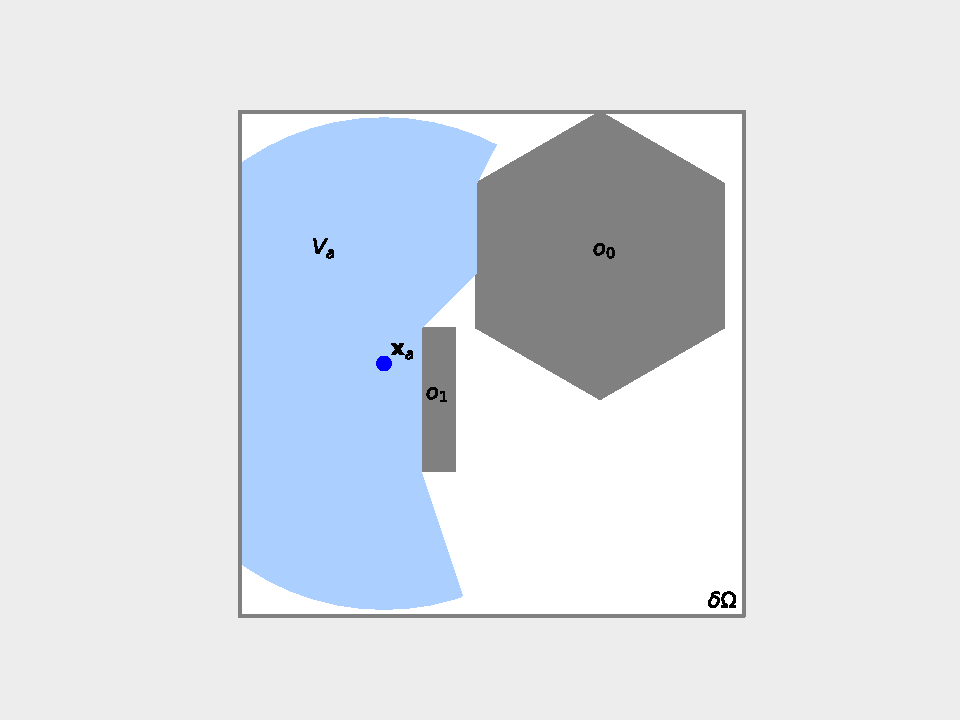
\includegraphics[width=\textwidth]{figs/vis_set_example.pdf}
  \caption{Visible set (light blue) for the agent placed at $\mathbf{x}_{a}$ in a rectangular mission space $\Omega$ with two obstacles ($\mathcal{O} = \{o_{0}, o_{1}\}$)}
  \label[fig]{vis_set_example}
\end{figure}
\todo{Update figure: $\mathbf{s}_{i}$ should be $\mathbf{x}_{a}$}
\subsection{Swarm}
A \textit{swarm}, $\mathcal{S}$ of size $N$ is a set of agents $\{a_{0}\hdots a_{N-1}\}$. The state of the swarm is described by the state of its participants 
, and is expressed as vector $\mathbf{x}_{\mathcal{S}}\in\mathbb{R}^{2N}$ as shown in \eqref{swarm_state_def}.
\begin{equation}\label[eq]{swarm_state_def}
  \mathbf{x}_{\mathcal{S}} = \begin{bmatrix}
    \mathbf{x}_{a_{0}}\\\vdots\\\mathbf{x}_{a_{N-1}}
  \end{bmatrix}
\end{equation}
The maximum radii of communication of the swarm are represented as the vector $\mathbf{r}\in\mathbb{R}^{N}$ as shown in \eqref{swarm_radii_def}.
\begin{equation}\label[eq]{swarm_radii_def}
  \mathbf{r}_{\mathcal{S}} = \begin{bmatrix}
    r_{a_{0}}&\hdots&r_{a_{N-1}}
  \end{bmatrix}^{T}
\end{equation}
Assuming that the distributions for all agents in the swarm are independent lets us use (7) in \cite{10.2307/24304959} to express 
the probability of $n$ members in the swarm, $\mathcal{S}$, being able to communicate with an entity at a point $\mathbf{y}$:
\begin{equation}\label[eq]{Phi_def}
  \Phi^{n}_{\mathcal{S}}(\mathbf{y}) = Pr(N_{com}(\mathcal{S}, \mathbf{y}) = n) = \sum_{A\in Comb(\mathcal{S}, n)}\prod_{a\in\mathcal{A}}\hat{p}(\mathbf{x}_{a}, \mathbf{y}, r_{a})\prod_{a\in\mathcal{S}\setminus\mathcal{A}}\big(1-\hat{p}(\mathbf{x}_{a}, \mathbf{y}, r_{a})\big)
\end{equation}
Later we will use the probability of \textit{at least} n members in a swarm beign able to communicate with an entity placed at $\mathbf{y}$, which is defined as:
\begin{equation}
  \begin{split}
    \Phi^{n^{+}}_{\mathcal{S}}(\mathbf{y}) &= Pr(N_{com}(\mathcal{S}, \mathbf{y}) \geq n) = 1 - \sum_{i=0}^{n-1}Pr(N_{com}(\mathcal{S}, \mathbf{y}) = i)\\
    &= 1 - \sum_{i=0}^{n-1}\Phi^{i}_{\mathcal{S}}(\mathbf{y})
  \end{split}
\end{equation}
\section{Problem formulation}
Using a swarm of $N$ mobile agents we want to set up a network in a mission space where the agents work as beacons in order to deliver precise positional data to entities entering the mission space.
\todo{skriv om at det er ønskelig å gjøre dette distribuert}
\subsection{Multilateration}\label[ssec]{trilat}
Multilateration is the process of determining the positions of unknown points in space by measurements of distances from known points \cite{trilat_website}. In order
to perform this task in two-dimensional space, at least three known points are needed.


Given $n\geq 3$ beacons located at positions $\mathbf{x}_{a}\in\mathbb{R}^{2},\; 0\leq a<n$ where not all points
lie on a single line the location 
of an entity, denoted by $\mathbf{y}\in\mathbb{R}^{2}$, can be determined as follows:
\begin{enumerate}
  \item The entity broadcasts signal and starts a timer at $t_{0}$.
  \item Beacons at $\mathbf{x}_{a},\; 0\leq a<n$ receive broadcasted signal and immediately responds with a packet containing $\mathbf{x}_{a}$.
  \item When receiving the packet from beacon at $\mathbf{x}_{a}$, the entity stores the time of reception in a variable $t_{1, a}$.
  \item When at least 3 beacons have responded, the entity calculates the distance
  from itself to beacon at $\mathbf{x}_{a}$: $d_{a} = \frac{1}{2}s(t_{1, a} - t_{0})$, where $s$ is the propagation speed of the signal. The factor $\frac{1}{2}$ is due to the signal traveling
  two times the distance between the entity and the beacon placed at $\mathbf{x}_{a}$ (the ping travels from the entity to the agent, and the packet
  sent by the agent travels back again).
  \item Based on the distances, $d_{a}$, and the positions of the beacons the entity can
  determine its position by calculating the point where circles centered at $\mathbf{x}_{a}$ with radii $d_{a}$ intersect.
\end{enumerate}
If sufficiently many beacons respond an ML (Maximum Likelihood) estimator of the position of the entity can be computed \cite{10.1145/381677.381693}.
Defining the error function:\begin{equation}
  e_{a}(\mathbf{y}) = s(t_{1, a} - t_{0, a}) - \norm{\mathbf{x}_{a} - \mathbf{y}} = d_{a} - \norm{\mathbf{x}_{a} - \mathbf{y}}
\end{equation}
We obtain the estimate for the position of the entity by solving:
\begin{equation}
  \mathbf{y}_{\mathrm{MMSE}} = \min_{\mathbf{y}} \mathbf{E}^{T}\mathbf{E},\quad\mathbf{E} = \begin{bmatrix}
    e_{0}(\mathbf{y})\\
    \vdots\\
    e_{n-1}(\mathbf{y})
  \end{bmatrix}
\end{equation}
The position estimation error is affected by the measurement errors, by the geometry relating sensors and target, and by the estimation algorithm \cite{trilat_error}.
As the pings sent by the entity that is to be located travel at large velocities (speed of light) the resolution of the internal clock of the entity sets a bound on the accuracy of the estimated position.
As was found in \cite{CRB_multilat}, multilateration of the unknown position of an entity is most accurate when the entity is placed nearby or within the convex hull of the beacons. Hence spreading
the beacons is desirable.
\figref{trilat_example} shows how the position of an entity can be determined from the known positions of 3 agents.
\begin{figure}[H]
  \centering
  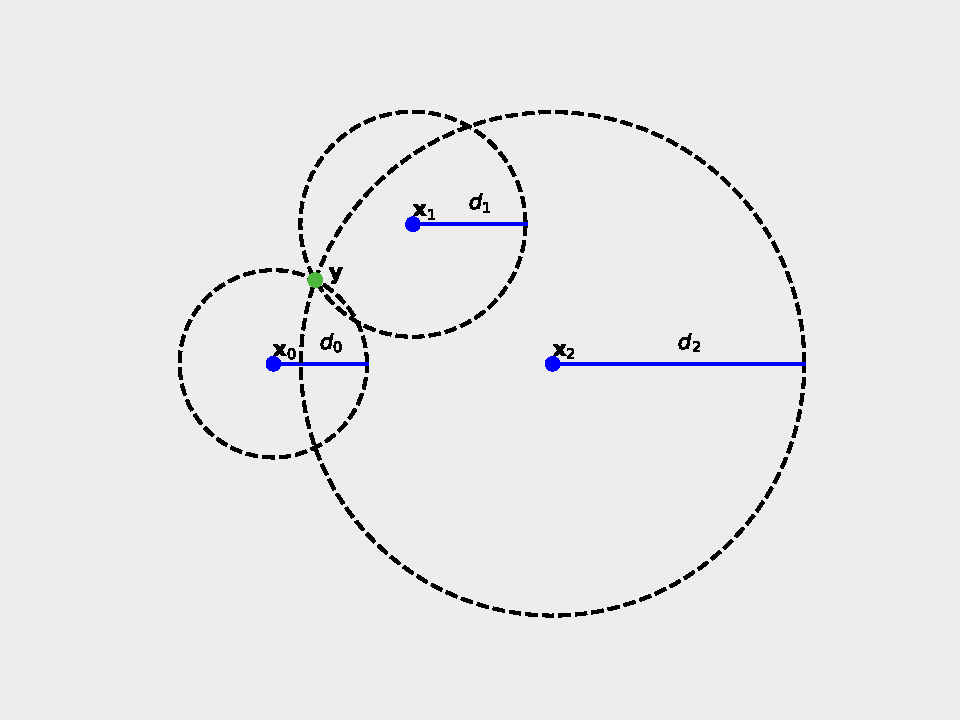
\includegraphics[width=.7\textwidth]{figs/trilateration_example.pdf}
  \caption{Position, $\mathbf{y}$, of entity determined by trilateration using known positions of $n = 3$ beacons.}
  \label[fig]{trilat_example}
\end{figure}

\subsection{Coverage}\label[secc]{coverage}
It is clear from subsection \ref{trilat} that three or more agents are needed to perform the task of multilateration. Hence a point $\mathbf{y}\in\mathcal{F}$ is said
to be \textit{covered} iff. it is within communication range of at least three agents, i.e. it is possible to determine the position of an entity placed at $\mathbf{y}$ through multilateration.

As discussed in subsection \ref{trilat} it is beneficial that agents used for multilateration spread out to some extent in order to ensure sufficient accuracy of multilateration.

\subsection{Objective function derivation}\label[secc]{obj_formulation}
The objective function presented here is inspired by \cite{sun2014escaping}, but differs in that for the purpose of multilateration, it is required that at least three agents must be within
range of a point in order for the point to be covered.

We assume we have a total of $N$ agents in a swarm $\mathcal{N}$ at our disposal. Furthermore we assume that all agents have the same maximum radius of communication:
\begin{equation}\label[eq]{homogenous_r}
  \begin{split}
    r_{a} &= r\;\forall\; a\in\mathcal{N}\\
  \end{split}
\end{equation}
Using \eqref{more_than_n_prob} we can express the probability of a point $\mathbf{y}$ being covered by the swarm as:
\begin{equation}\label[eq]{cover_prob}
  \Phi^{3^{+}}(\mathbf{X}_{\mathcal{N}}, \mathbf{y}) = 1 - \Phi^{0}(\mathbf{X}_{\mathcal{N}}, \mathbf{y}) - \Phi^{1}(\mathbf{X}_{\mathcal{N}}, \mathbf{y}) - \Phi^{2}(\mathbf{X}_{\mathcal{N}}, \mathbf{y})
\end{equation}
In order to formulate a distributed optimization algorithm, we rewrite the probability of coverage in \eqref{cover_prob} with focus on a single drone $a$.
We partition the swarm, $\mathcal{N}$, into two disjoint sets: $\{a\}$ and $\mathcal{N}\setminus\{a\}$. Using this we can rewrite \eqref{cover_prob} as:
\begin{equation}\label[eq]{distr_cover_derivation}
  \begin{split}
    \Phi^{3^{+}}(\mathbf{X}_{\mathcal{N}}, \mathbf{y}) &= 1\\
    &- \big(1-\hat{p}(\mathbf{x}_{a}, \mathbf{y})\big)\prod_{k\in\mathcal{N}\setminus\{a\}}\big(1-\hat{p}(\mathbf{x}_{k}, \mathbf{y}))\\
    &- \hat{p}(\mathbf{x}_{a}, \mathbf{y})\prod_{k\in\mathcal{N}\setminus\{a\}}\big(1-\hat{p}(\mathbf{x}_{k}, \mathbf{y}))\\
    &- \big(1-\hat{p}(\mathbf{x}_{a}, \mathbf{y})\big)\sum_{j\in\mathcal{N}\setminus\{a\}}\hat{p}(\mathbf{x}_{j}, \mathbf{y})\prod_{k\in\mathcal{N}\setminus\{a\}\setminus\{j\}}\big(1-\hat{p}(\mathbf{x}_{k}, \mathbf{y})\big)\\
    &- \hat{p}(\mathbf{x}_{a}, \mathbf{y})\sum_{j\in \mathcal{N}\setminus\{a\}}\hat{p}(\mathbf{x}_{j}, \mathbf{y})\prod_{k\in\mathcal{N}\setminus\{a\}\setminus\{j\}}\big(1-\hat{p}(\mathbf{x}_{k}, \mathbf{y})\big)\\
    &- \big(1-\hat{p}(\mathbf{x}_{a}, \mathbf{y})\big)\sum_{\mathcal{A}\in Comb(\mathcal{N}\setminus\{a\}, 2)}\prod_{j\in\mathcal{A}}\hat{p}(\mathbf{x}_{j}, \mathbf{y})\prod_{k\in\mathcal{N}\setminus\{a\}\setminus\mathcal{A}}\big(1-\hat{p}(\mathbf{x}_{k}, \mathbf{y})\big)\\
    &= 1\\
    &- \prod_{k\in\mathcal{N}\setminus\{a\}}\big(1-\hat{p}(\mathbf{x}_{k}, \mathbf{y}))\\
    &- \sum_{j\in\mathcal{N}\setminus\{a\}}\hat{p}(\mathbf{x}_{j}, \mathbf{y})\prod_{k\in\mathcal{N}\setminus\{a\}\setminus\{j\}}\big(1-\hat{p}(\mathbf{x}_{k}, \mathbf{y})\big)\\
    &- \big(1-\hat{p}(\mathbf{x}_{a}, \mathbf{y})\big)\sum_{\mathcal{A}\in Comb(\mathcal{N}\setminus\{a\}, 2)}\prod_{j\in\mathcal{A}}\hat{p}(\mathbf{x}_{j}, \mathbf{y})\prod_{k\in\mathcal{N}\setminus\{a\}\setminus\mathcal{A}}\big(1-\hat{p}(\mathbf{x}_{k}, \mathbf{y})\big)\\
  \end{split}
\end{equation}
Applying \eqref{Phi_def} to \eqref{distr_cover_derivation} yields:
\begin{equation}\label[eq]{local_coverage}
  \begin{split}
    \Phi^{3^{+}}(\mathbf{X}_{\mathcal{N}}, \mathbf{y}) &= 1 - \Phi^{0}(\mathbf{X}_{\mathcal{N}\setminus\{a\}}, \mathbf{y}) - \Phi^{1}(\mathbf{X}_{\mathcal{N}\setminus\{a\}}, \mathbf{y}) - \Phi^{2}(\mathbf{X}_{\mathcal{N}\setminus\{a\}}, \mathbf{y})\big(1-\hat{p}(\mathbf{x}_{a}, \mathbf{y})\big)\\
    &= \Phi^{3^{+}}(\mathbf{X}_{\mathcal{N}\setminus\{a\}}, \mathbf{y}) + \Phi^{2}(\mathbf{X}_{\mathcal{N}\setminus\{a\}}, \mathbf{y})\hat{p}(\mathbf{x}_{a}, \mathbf{y})\\
  \end{split}
\end{equation}
Rewriting \eqref{local_coverage} yields:
\begin{equation}
  \begin{split}
    \Phi^{3^{+}}(\mathbf{X}_{\mathcal{N}}, \mathbf{y}) &= \Phi^{3^{+}}(\mathbf{X}_{\mathcal{N}\setminus\{a\}}, \mathbf{y}) - \hat{p}(\mathbf{x}_{a}, \mathbf{y})\Phi^{3^{+}}(\mathbf{X}_{\mathcal{N}\setminus\{a\}}, \mathbf{y}) + \hat{p}(\mathbf{x}_{a}, \mathbf{y})\Phi^{2^{+}}(\mathbf{X}_{\mathcal{N}\setminus\{a\}}, \mathbf{y})\\
    &= (1-\hat{p}(\mathbf{x}_{a}, \mathbf{y}))\Phi^{3^{+}}(\mathbf{X}_{\mathcal{N}\setminus\{a\}}, \mathbf{y}) + \hat{p}(\mathbf{x}_{a}, \mathbf{y})\Phi^{2^{+}}(\mathbf{X}_{\mathcal{N}\setminus\{a\}}, \mathbf{y})\\
  \end{split}
\end{equation}
It is clear that the probability of the point $\mathbf{y}$ being covered can be seen on as an interpolation between two probability measures with the local probability of agent $a$ as the interpolation variable. Low local probability of agent $a$ means that the probability of coverage supplied the swarm as a whole depends more on the coverage supplied by
the swarm excluding agent $a$. In the extreme case where the local probability of agent $a$ is zero, the probability of covering $\mathbf{y}$ depends only on the coverage supplied by the swarm excluding agent $a$.

Higher local probability of agent $a$ means that the contribution of $a$ towards covering the point $\mathbf{y}$ is greater, thus less weight is put on the the probability of the swarm excluding agent $a$ covering the point. Instead more weight is put on the probability of at least \textit{two} other agents being able to communicate with an entity at $\mathbf{y}$. 
This is due to the fact that the probability of agent $a$ being able to communicate with said entity is higher, and we need only two or more other agents to be able to communicate with the entity at $\mathbf{y}$ to make the total number of agents covering $\mathbf{y}$ three or more.

\begin{figure}[H]
  \centering
  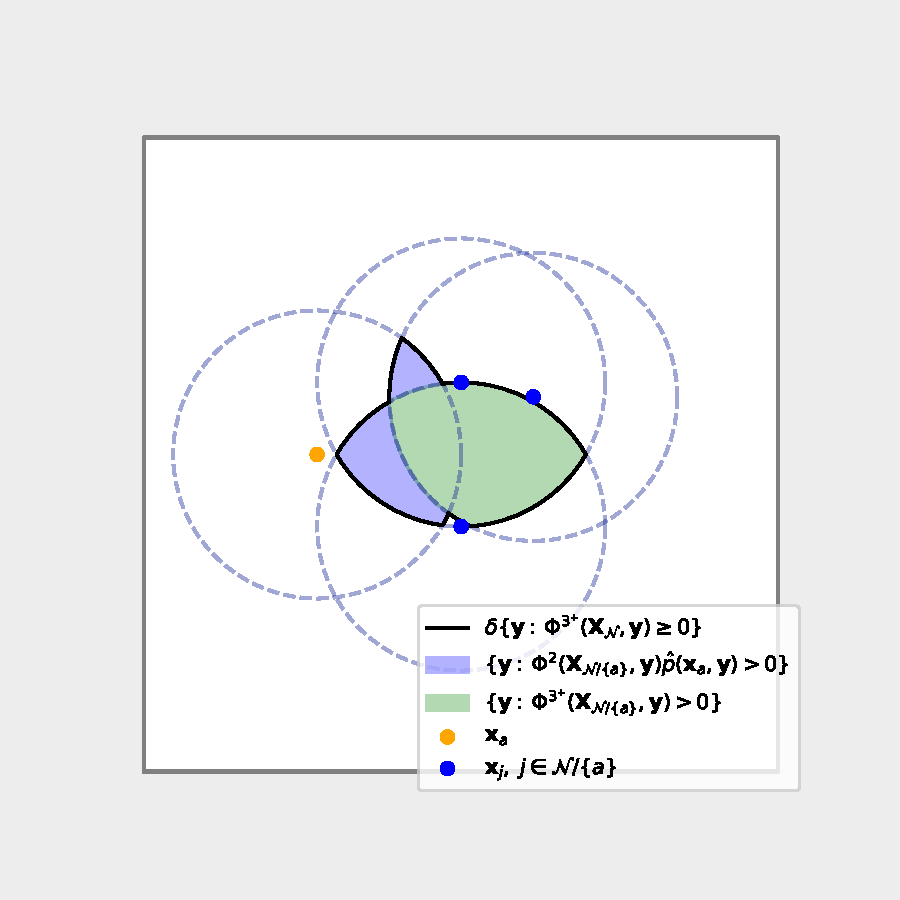
\includegraphics[width=.75\textwidth]{figs/local_objective_example.pdf}
  \caption{Non-zero regions of integrads in \eqref{rewritten_objective}. Note that perturbing the orange circle (position of agent $a$) does not affect the green region,
  as it is defined only by the intersections of the disks surrounding the blue points (other agents in the swarm).}
  \label[fig]{local_coverage_example}
\end{figure}

We note that the overall probability of coverage over the feasible space can be written as:
\begin{equation}\label[eq]{rewritten_objective}
  \begin{split}
    P(\mathbf{X}_{\mathcal{N}}) &=\int_{\mathcal{F}}\Phi^{3^{+}}(\mathbf{X}_{\mathcal{N}}, \mathbf{y})d\mathbf{y} =  \int_{\mathcal{F}}\Phi^{3^{+}}(\mathbf{X}_{\mathcal{N}\setminus\{a\}}, \mathbf{y}) + \Phi^{2}(\mathbf{X}_{\mathcal{N}\setminus\{a\}}, \mathbf{y})\hat{p}(\mathbf{x}_{a}, \mathbf{y})d\mathbf{y}\\
    &= \int_{\mathcal{F}}\Phi^{3^{+}}(\mathbf{X}_{\mathcal{N}\setminus\{a\}}, \mathbf{y})d\mathbf{y} + \int_{\mathcal{F}}\Phi^{2}(\mathbf{X}_{\mathcal{N}\setminus\{a\}}, \mathbf{y})\hat{p}(\mathbf{x}_{a}, \mathbf{y})d\mathbf{y}\\
  \end{split}
\end{equation}
We note that the first term in \eqref{rewritten_objective} is independent of the position of $a$ in both its domain and integrand. This independence is visualized in \figref{local_coverage_example}. Thus we can rewrite the overall coverage probability over $\mathcal{F}$ as:
\begin{equation}
  P(\mathbf{X}_{\mathcal{N}}) = P(\mathbf{X}_{\mathcal{N}\setminus\{a\}}) + P_{a}(\mathbf{X}_{\mathcal{N}})
\end{equation}
Where the \textit{local} probability of coverage for agent $a$ over the feasible space is defined as:
\begin{equation}\label[eq]{local_objective}
  P_{a}(\mathbf{X}_{\mathcal{N}}) = \int_{\mathcal{F}}\Phi^{2}(\mathbf{X}_{\mathcal{N}\setminus\{a\}}, \mathbf{y})\hat{p}(\mathbf{x}_{a}, \mathbf{y})d\mathbf{y}
\end{equation}

As in \cite{sun2014escaping} we note that from the viewpoint of agent $a$, the swarm can be partitioned into three disjoint sets: $\{a\}$, $\mathcal{B}_{a}$ and $\mathcal{C}_{a}$. The latter sets are defined as:
\begin{subequations}\label[eq]{B_a_and_C_a_def}
  \begin{equation}\label[eq]{neigh_def}
    \mathcal{B}_{a} = \{j\in\mathcal{N}\setminus\{a\}: \norm{\mathbf{x}_{a}-\mathbf{x}_{j}} \leq 2r\}
  \end{equation}
  \begin{equation}
    \mathcal{C}_{a} = \{j\in\mathcal{N}\setminus\{a\}: \norm{\mathbf{x}_{a}-\mathbf{x}_{j}} > 2r\}
  \end{equation}  
\end{subequations}
The set $\mathcal{B}_{a}$, from now on called the neighbours of $a$, contains all agents in the swarm, $\mathcal{N}$, whose communication disks form a non-empty intersection with that of $a$.
$\mathcal{C}_{a}$ contains all agents whose communication disks do not intersect with that of $a$.

Applying \eqref{B_a_and_C_a_def} to \eqref{local_objective} yields:
\begin{equation}
  \begin{split}
    P_{a}(\mathbf{X}_{\mathcal{N}}) &= \int_{\mathcal{F}}\Phi^{2}(\mathbf{X}_{\mathcal{N}\setminus\{a\}}, \mathbf{y})\hat{p}(\mathbf{x}_{a}, \mathbf{y})d\mathbf{y}\\
    &= \int_{\mathcal{F}}\Big(\Phi^{2}(\mathbf{X}_{\mathcal{B}_{a}}, \mathbf{y}) + \Phi^{2}(\mathbf{X}_{\mathcal{C}_{a}}, \mathbf{y}) + \Phi^{1}(\mathbf{X}_{\mathcal{B}_{a}}, \mathbf{y})\Phi^{1}(\mathbf{X}_{\mathcal{C}_{a}}, \mathbf{y})\Big)\hat{p}(\mathbf{x}_{a}, \mathbf{y})d\mathbf{y}
  \end{split}
\end{equation}
Partitioning the domain of integration into the visible set and invisible set of agent $a$, and noting that $\hat{p}(\mathbf{x}_{j}, \mathbf{y}) = 0\;\forall\;j\in\mathcal{C}_{a},\;\mathbf{y}\in V_{a}$ such that
$\Phi^{n}(\mathbf{X}_{\mathcal{C}_{a}}, \mathbf{y}) = 0\;\forall\;n\in\mathbb{Z}^{+},\;\mathbf{y}\in V_{a}$, and $\hat{p}(\mathbf{x}_{a}, \mathbf{y}) = 0\;\forall\;\mathbf{y}\in U_{a}$ yields:
\begin{equation}\label[eq]{local_objective_derivated}
  \begin{split}
    P_{a}(\mathbf{X}_{\mathcal{N}}) &= \int_{V_{a}}\Big(\Phi^{2}(\mathbf{X}_{\mathcal{B}_{a}}, \mathbf{y}) + \Phi^{2}(\mathbf{X}_{\mathcal{C}_{a}}, \mathbf{y}) + \Phi^{1}(\mathbf{X}_{\mathcal{B}_{a}}, \mathbf{y})\Phi^{1}(\mathbf{X}_{\mathcal{C}_{a}}, \mathbf{y})\Big)\hat{p}(\mathbf{x}_{a}, \mathbf{y})d\mathbf{y}\\
    &+ \int_{U_{a}}\Big(\Phi^{2}(\mathbf{X}_{\mathcal{B}_{a}}, \mathbf{y}) + \Phi^{2}(\mathbf{X}_{\mathcal{C}_{a}}, \mathbf{y}) + \Phi^{1}(\mathbf{X}_{\mathcal{B}_{a}}, \mathbf{y})\Phi^{1}(\mathbf{X}_{\mathcal{C}_{a}}, \mathbf{y})\Big)\hat{p}(\mathbf{x}_{a}, \mathbf{y})d\mathbf{y}\\
    &= \int_{V_{a}}\Phi^{2}(\mathbf{X}_{\mathcal{B}_{a}}, \mathbf{y})p(\norm{\mathbf{x}_{a}-\mathbf{y}})d\mathbf{y} = L(\mathbf{X}_{\mathcal{B}_{a}\cup\{a\}})
  \end{split}
\end{equation}
Thus the local probability of coverage for an agent $a$ is dependent on the position, $\mathbf{x}_{a}$, of agent $a$ in both domain and integrand, and the positions of the neighbours of agent $a$.
We call the swarm consisting of $a$ and its neighbours agent $a$'s local swarm.\clearpage

In order to encourage spread of agents in situations where small perturbations of the position of an agent
causes no or minor changes to the local probability of coverage, we introduce a term causing an agent $a$ to move away
from another agent $j$. When agents are close to each other we want this term to induce some velocity in the agents causing
them to spread. Furthermore we want this velocity to decrease with increasing spread. Due to this we model the proximity of two agents as:
\begin{equation}\label[eq]{proximity_func}
  D(\mathbf{x}_{a}, \mathbf{x}_{j}) = k_{1}e^{-k_{2}\norm{\mathbf{x}_{a} - \mathbf{x}_{j}}}
\end{equation}
The function has two tunable parameters, $k_{1}$ and $k_{2}$, whose effects are show in \figref{cdr}.

Using \eqref{local_objective_derivated} and \eqref{proximity_func}  We now state the \textit{local} objective for an agent $a$ as:
\begin{equation}\label[eq]{local_objective_func}
  H(\mathbf{X}_{\mathcal{B}_{a}\cup\{a\}})  = L(\mathbf{X}_{\mathcal{B}_{a}\cup\{a\}})  - \sum_{j\in\mathcal{B}_{a}}D(\mathbf{x}_{a}, \mathbf{x}_{j})
\end{equation}
Due to the negative sign in front of the sum of proximity functions, we will refer to this as the active dispersion term.
\begin{figure}[H]
  \centering
  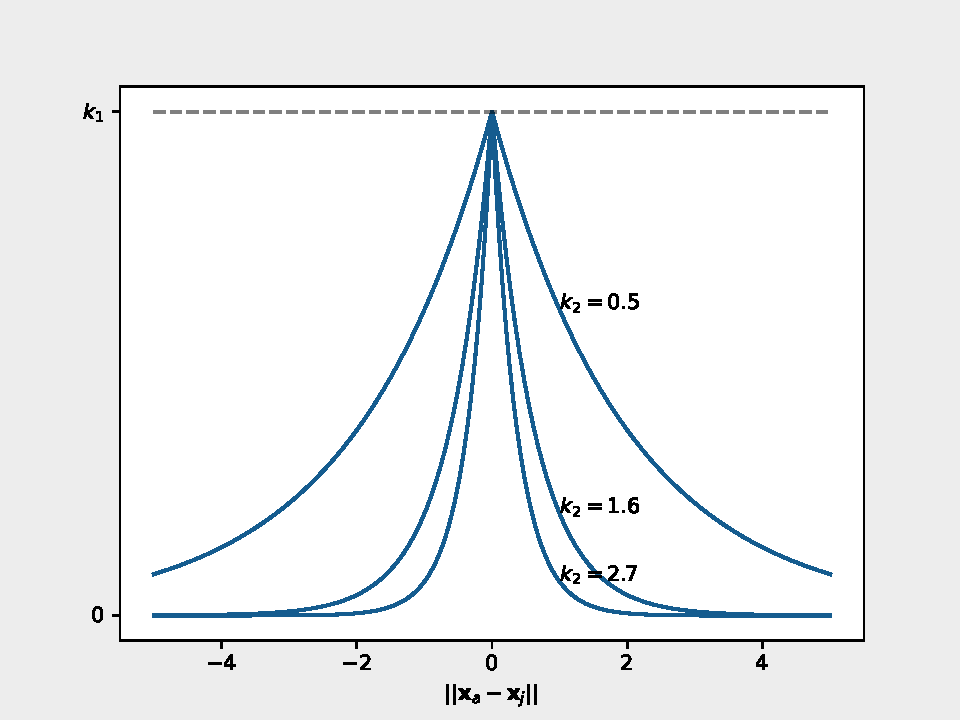
\includegraphics[width=.7\textwidth]{figs/close_dist_repell_example.pdf}
  \caption{Proximity term in \eqref{proximity_func} for an agent, $a$, and its neighbour, $j$.}
  \label[fig]{cdr}
\end{figure}

\subsection{Constraints}\label[secc]{constraints}
It is clear from subsection \ref{trilat} that agents used as beacons in a multilateration scheme cannot be positioned on a straight line, as this would make it impossible
to uniquely determine the unknown position of an entity. Due to the fact that only agents close to the entity whose position is to be determined will
take part in the multilateration scheme, we impose only that agents that together can be used for multulateration must satisfy the non-linear position requirement.

For an agent $a$ with $N$ neighbours $j\in\mathcal{B}_{a},\:|B_{a}|=N$ we construct a matrix $\mathbf{V}$ according to:
\begin{equation}\label[eq]{V_def}
  \mathbf{V}(\mathbf{X}_{\mathcal{B}_{a}}) = \begin{bmatrix}
    \mathbf{X}_{\mathcal{B}_{a, 0}}-\mathbf{X}_{\mathcal{B}_{a, 1}}&\hdots&\mathbf{X}_{\mathcal{B}_{a, 0}}-\mathbf{X}_{\mathcal{B}_{a, N-1}}.
  \end{bmatrix}
\end{equation}
If agent $a$ has less than two neighbours, or all of agent $a$'s neighbours are positioned on a straight line, the matrix $\mathbf{V}(\mathbf{X}_{\mathcal{B}_{a}})$ will not span $\mathbb{R}^{2}$, i.e. $\mathrm{Rank}(\mathbf{V}(\mathbf{X}_{\mathcal{B}_{a}})) < 2$ \todo{citation for matrix rank}.

Assuming that agent a has two or more agents, $|\mathcal{B}_{a}|\geq 2$, and that all neighbours of $a$ are positioned on a straight line. It is then desirable that agent $a$ is positioned sufficiently far away from the line. This constraint is implemented as follows:
Wihout loss of generality we define:
\begin{subequations}\label[eq]{vl}
  \begin{align}
    \mathbf{v}(\mathbf{x}_{a}) &= \mathbf{x}_{a} - \mathbf{X}_{\mathcal{B}_{a}, 0}\\
    \mathbf{l} &= \mathbf{X}_{\mathcal{B}_{a}, 1} - \mathbf{X}_{\mathcal{B}_{a}, 0},
  \end{align}
\end{subequations}
meaning $\mathbf{v}(\mathbf{x}_{a})$ is the vector from agent $a$ to its first neighbour, and $\mathbf{l}$ is the vector between agent $a$'s first and second neighbour. Thus $\mathbf{l}$ is paralell to the line 
that goes through all of agent $a$'s neighbours.
Using (3.98) in \cite{projection} to project $\mathbf{v}(\mathbf{x}_{a})$ into $\mathbf{l}$ we get the component of $\mathbf{v}(\mathbf{x}_{a})$ that is parallel to the line
through agent $a$'s neighbour $i$ and $j$:
\begin{equation}
  \mathbf{v}_{\parallel}(\mathbf{x}_{a}) = \frac{\mathbf{v}(\mathbf{x}_{a})^{T}\mathbf{l}}{\mathbf{l}^{T}\mathbf{l}}\mathbf{l}
\end{equation}
The component of $\mathbf{v}(\mathbf{x}_{a})$ perpendicular to the line through agent $a$'s
neighbours is obtained as:
\begin{equation}
  \mathbf{v}_{\perp}(\mathbf{x}_{a}) = \mathbf{v}(\mathbf{x}_{a}) - \mathbf{v}_{\parallel}(\mathbf{x}_{a})
\end{equation}
Now the distance from agent $a$ to the line through its neighbours can be computed as:
\begin{equation}
  \norm{\mathbf{v}_{\perp}(\mathbf{x}_{a})} = \norm{\mathbf{v}(\mathbf{x}_{a}) - \frac{\mathbf{v}(\mathbf{x}_{a})^{T}\mathbf{l}}{\mathbf{l}^{T}\mathbf{l}}\mathbf{l}}
\end{equation}
Seen as it is impossible to place and agent such that it lays on a straight line through all it's neighbours if the neigbhours do not already
lay on a straight line we demand that the non-linear position constraint be fulfilled only when $\mathrm{Rank}(\mathbf{V}(\mathbf{X}_{\mathcal{B}_{a})}) < 2$, where $\mathbf{V}(\cdot)$ is defined in \eqref{V_def}. The non-linear position constraint is defined as:
\begin{equation}\label[eq]{non_lin_pos}
    \norm{\mathbf{v}(\mathbf{x}_{a}) - \frac{\mathbf{v}(\mathbf{x}_{a})^{T}\mathbf{l}}{\mathbf{l}^{T}\mathbf{l}}\mathbf{l}}\geq d_{min} 
\end{equation}
where $d_{min}$ is a tunable parameter that defines how close an agent is allowed get to the line through it's neigbhours, and $\mathbf{v}$ and $\mathbf{l}$
are defined in \eqref{vl}.

We also impose that any two agents must be some minimum distance apart at any given time. This is due to the fact that agents colliding could cause damage to the hardware, and possibly render them unusable.
This constraint is modelled as:
\begin{equation}
  \norm{\mathbf{x}_{a} - \mathbf{x}_{j}} \geq r_{min} \;\forall\;j\in\mathcal{B}_{a},
\end{equation}
where $r_{min}$ is a tunable parameter that sets a limit to how close an agent can be positioned to any of its neihbours.\clearpage
\subsection{Optimization problem formulation}
The non-linear position constraint \eqref{non_lin_pos} presented in \ref{constraints} is dependent on the neighbour set of agent $a$, $\mathcal{B}_{a}$, as it should only be imposed if the 
neigbours of agent $a$ lay on a straight line. Using the objective function in \eqref{local_objective_func} and the constraints in discussed in \ref{constraints} we define the optimization problem:
\begin{subequations}\label[eq]{local_opt_prob}
  \begin{align}
    \begin{split}\label[eq]{totally_objective}
      &\max_{\mathbf{x}_{a}}\;H(\mathbf{X}_{\mathcal{B}_{a}\cup\{a\}})\\
    \end{split}\\
    \mathrm{s.t.}\;
    \begin{split}
      &\mathbf{x}_{a}\in\mathcal{F}
    \end{split}\\
    \begin{split}\label[eq]{min_two_neig}
      &|\{j\in\mathcal{B}_{a}: \norm{\mathbf{x}_{a} - \mathbf{x}_{j}} \leq 2r\}|\geq 2
    \end{split}\\
    \begin{split}
      &\norm{\mathbf{x}_{a} - \mathbf{x}_{j}} \geq r_{min}\;\forall\;j\in\mathcal{B}_{a}
    \end{split}\\
    \begin{split}\label[eq]{non_linear_neighb}
      &\norm{\mathbf{v}(\mathbf{x}_{a}) - \frac{\mathbf{v}(\mathbf{x}_{a})^{T}\mathbf{l}}{\mathbf{l}^{T}\mathbf{l}}\mathbf{l}}\geq d_{min},\quad\mathrm{iff.}\;\mathrm{Rank}(\mathbf{V}(\mathbf{X}_{\mathcal{B}_{a}}))<2
    \end{split}
\end{align}
\end{subequations}
where $\mathbf{V}(\cdot)$ is defined in \eqref{V_def} and $\mathbf{v}(\cdot)$ and $\mathbf{l}$ are defined in \eqref{vl}.

In situations where $\frac{\partial L(\mathbf{X}_{\mathcal{B}_{a}\cup\{a\}})}{\partial \mathbf{x}_{a}} = 0$ the solution of \eqref{totally_objective} will be achieved at the position $\mathbf{x}_{a}$ that minimizes the dispersion term in \eqref{local_objective_func}.
This will cause agent $a$ to move as far away from its neighbours as possible. Such behaviour is undesirable as this might render agent $a$ neighbour-less. For an agent 
$a$ without neighbous we have $\mathcal{B}_{a} = \emptyset$ and hence $H(\mathbf{X}_{\mathcal{B}_{a}\cup\{a\}}) \equiv 0$. Thus re-optimization will result in $\mathbf{x}_{a}$ being unaltered, causing agent $a$
to stay at $\mathbf{x}_{a}$ indefinately. To prevent such behaviour we impose the constraint \eqref{min_two_neig}. This will prevent agent $a$ from completely disconnecting from its local swarm. 

Furthermore we observe that Rank$(\mathbf{V}(\mathbf{X}_{\mathcal{B}_{a}}))<2$ if either all neigbhours of agent $a$ lie on a straight line or agent $a$ has less than two neighbours. If agent $a$ has less than
two neighbours it is not possible to draw a line between the neighbours of agent $a$, and thus the non-linear neighbour constraint \eqref{non_linear_neighb} is undefined. This further motivates imposing the constraint that
agent $a$ should have at least two neighbours at the solution to \eqref{local_opt_prob}.

The optimization problem formulated in \eqref{local_opt_prob} is non-convex \cite{NoceWrig06_convex_prob}. The objective function is generally non-concave and the constraints form a non-convex feasible set. In 
\figref{objective_example} a visualization of the objective function is shown for an agent with 5 neighbours.
\begin{figure}[H]
  \centering
  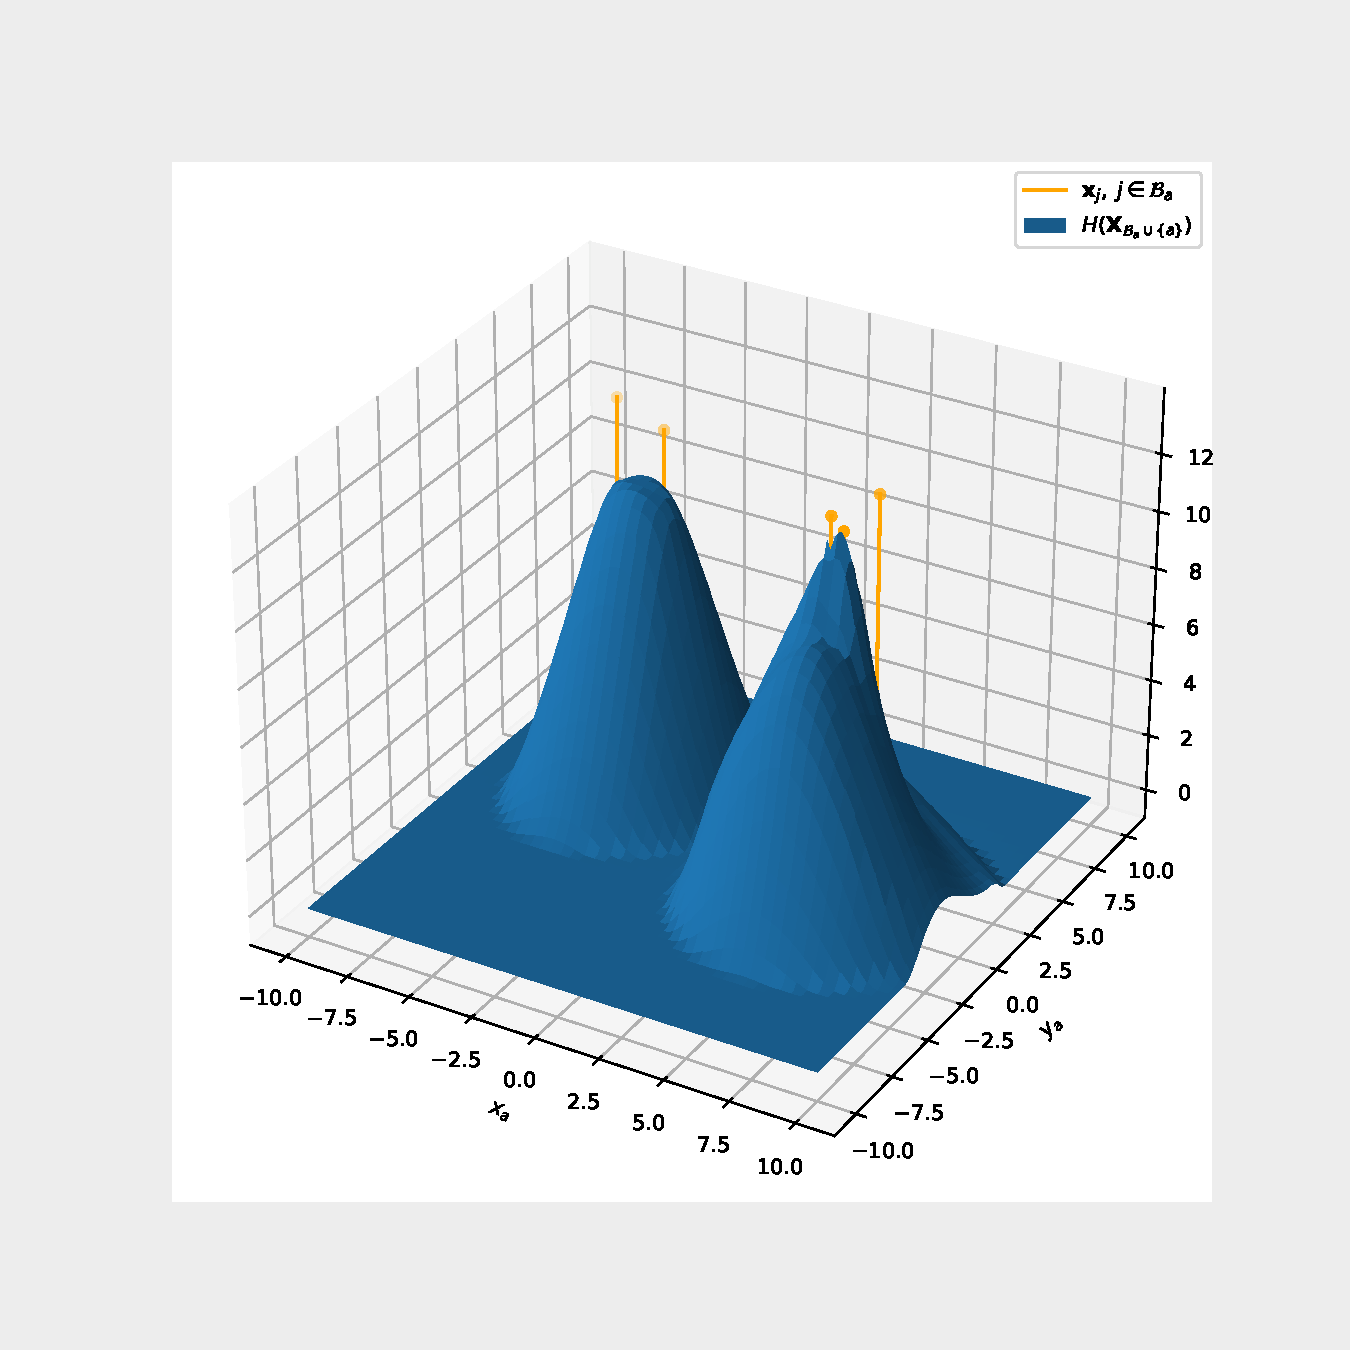
\includegraphics[width = .8\textwidth]{figs/objective_example.pdf}
  \caption{Objective function in \eqref{totally_objective} for agent $a$ with $|B_{a}| = 5$.}
  \label[fig]{objective_example}
\end{figure}
\section{Implementation}
\subsection{Local probability}
It is assumed that the agents have perfect communication capabilities within their maximum range. The local probability of an agent $a$ wrt. a point $\mathbf{y}$ is defined as:
\begin{equation}
  \hat{p}(\mathbf{x}_{a}, \mathbf{y}) = \begin{cases}
    1, &\mathbf{y}\in V_{a}\\
    0, &\mathbf{y}\in U_{a}
  \end{cases} = 1_{\big\{\mathbf{y}\in V_{a}\big\}},
\end{equation}
where $1_{\{\cdot\}}$ is the indicator function, which is simply equal to one if the clause in the subscript is true and zero otherwise.
This implies that the overall probability of coverage over the feasible space in \eqref{rewritten_objective} is simply the area of all intersections of three or more visible sets.

\subsection{Computing the local probability of coverage}
The neighbors of an agent $a$ is partitioned into two sets:
\begin{subequations}
  \begin{equation}
    \mathcal{B}_{a V} = \{j\in\mathcal{B}_{a}: \mathbf{y}\in V_{j}\}
  \end{equation}
  \begin{equation}
    \mathcal{B}_{a U} = \{j\in\mathcal{B}_{a}: \mathbf{y}\in U_{j}\}.
  \end{equation}
\end{subequations}
Thus for a given point $\mathbf{y}$, the set $\mathcal{B}_{a V}$ contains all neighbors of $a$ whose visible set contains $\mathbf{y}$,
and $\mathcal{B}_{a U}$ contains all neighbors of agent $a$ whose visible set does not contain $\mathbf{y}$.

Now the local probability of coverage for agent $a$ can be written as:
\begin{equation}\label[eq]{loc_prob_cov_implt}
  \begin{split}
    L(\mathbf{X}_{\mathcal{B}_{a}\cup\{a\}}) &= \int_{V_{a}}\Phi^{2}(\mathbf{X}_{\mathcal{B}_{a}}, \mathbf{y})1_{\{\mathbf{y}\in V_{a}\}}d\mathbf{y} = \int_{V_{a}}\Phi^{2}(\mathbf{X}_{\mathcal{B}_{a}}, \mathbf{y})d\mathbf{y}\\
    &= \int_{V_{a}}\sum_{n = 0}^{2} \Phi^{n}(\mathbf{X}_{\mathcal{B}_{a V}}, \mathbf{y})\Phi^{2-n}(\mathbf{X}_{\mathcal{B}_{a U}},\mathbf{y})d\mathbf{y}\\
    &= \int_{V_{a}}\sum_{n = 0}^{2}1_{\{|B_{a V}| = n\}}1_{\{2-n = 0\}}d\mathbf{y}\\
    &= \int_{V_{a}}1_{\{|B_{a V}| = 2\}}d\mathbf{y}.
  \end{split}
\end{equation}
Thus the value of the local probability of coverage is equal to the area where the visible set of $a$ overlaps with those of exactly two neighboring agents when assuming perfect communication within the entire visible set.

An alternative way of computing the value of the local probability of coverage in \eqref{loc_prob_cov_implt}, used in the implementation,
is presented below:
\begin{equation}\label[eq]{two_neigh_area}
  \begin{split}
    L(\mathbf{X}_{\mathcal{B}_{a}\cup\{a\}}) &= A\Biggr(\bigcup_{\mathcal{A}\in \mathrm{Comb}(\mathcal{B}_{a}, 2)}\Bigg[\bigg(V_{a}\cap \bigcap_{i\in\mathcal{A}}V_{i}\bigg)\setminus\bigg(\bigcup_{j\in\mathcal{B}_{a}\setminus\mathcal{A}}V_{j}\bigg)\Bigg]\Biggr)\\
    &= A\Biggr(V_{a}\cap\bigcup_{\mathcal{A}\in \mathrm{Comb}(\mathcal{B}_{a}, 2)}\Bigg[\bigg(\bigcap_{i\in\mathcal{A}}V_{i}\bigg)\setminus\bigg(\bigcup_{j\in\mathcal{B}_{a}\setminus\mathcal{A}}V_{j}\bigg)\Bigg]\Biggr),
  \end{split}
\end{equation}
where $A(\cdot)$ returns the area of its argument.
\subsection{Optimizing swarm configuration}
Running simulations is done by iteratively solving \eqref{local_opt_prob} for one agent at a time. Meaning at any time there is only
a single agent computing its optimal position while all other agents are static. Once the agent currently computing its optimal position
has done so, it moves to the optimum. Then the next agent does the same, and so on. This procedure is repeated
until all agents are sufficiently close to a local optimum. The procedure is described in Algorithm \ref{alg:alg1}.

\begin{algorithm}[H]
  \SetAlgoLined
  \KwIn{Size of swarm: $N$, Initial configuration of swarm: $\mathbf{X}_{0}$, Feasible space: $\mathcal{F}$, Tolerance: $\epsilon$}

  $\mathbf{X}_{\mathcal{N}}\gets \mathbf{X}_{0}$\;
  \For{$a\gets 0$ \KwTo $N-1$}{
    $\mathbf{C}[a]\gets\mathrm{False}$\;
    $\mathbf{V}[a]\gets$ Compute $V_{a}$ using \eqref{visible_set_def} with $\mathbf{x}_{a} = \mathbf{X}_{\mathcal{N}}[a]$\;
  }
   \While{not $\mathbf{C}[a]$ is $\mathrm{True}$ for all $a = 0\hdots N-1$}{
     \For{$a\gets 0$ \KwTo $N-1$}{
       $\mathbf{x}_{a, 0}\gets\mathbf{X}_{\mathcal{N}}[a]$\;
       $\mathcal{B}_{a}\gets$ Compute $\mathcal{B}_{a}$ using \eqref{neigh_def} with $\mathbf{x}_{a} = \mathbf{x}_{a, 0}$\;
       $\mathbf{x}_{a}^{*}\gets$ Solve \eqref{local_opt_prob} with initial guess $\mathbf{x}_{a, 0}$ and neighbors $\mathcal{B}_{a}$\;
       \If{$\norm{\mathbf{x}_{a}^{*} - \mathbf{x}_{a, 0}}\leq\epsilon$}{
         $\mathbf{C}[a]\gets\mathrm{True}$
       }
       $\mathbf{V}[a]\gets$ Compute $V_{a}$ using \eqref{visible_set_def} with $\mathbf{x}_{a} = \mathbf{x}_{a}^{*}$\;
       $\mathbf{X}_{\mathcal{N}}[a]\gets\mathbf{x}_{a}^{*}$\;
     }
   }
   \KwRet{$\mathbf{X}_{\mathcal{N}}$}
   \caption{Optimizing swarm configuration}
   \label{alg:alg1}
  \end{algorithm}
\subsection{Optimization solver}
As \eqref{local_opt_prob} is a non-convex and constrained optimization problem it is solved using Sequential Quadratic Programming (SQP). 
In \cite{kraft1988software} a Nonlinear Program (NLP) is defined as:
\begin{equation}\label[eq]{nlp}
  \begin{split}
    \min_{\mathbf{x}\in\mathbb{R}^{n}}f(\mathbf{x})\quad\mathrm{s.t.}\quad&g_{i}(\mathbf{x}) = 0\;i\in\{1\hdots m_{e}\}\\
    &g_{i}(\mathbf{x}) \geq 0\;i\in\{m_{e}+1\hdots m\}\\
    &\mathbf{x}^{lb}\leq\mathbf{x}\leq\mathbf{x}^{ub}
  \end{split}
\end{equation}
where $f:\mathbb{R}^{n}\rightarrow\mathbb{R}$ and $g:\mathbb{R}^{n}\rightarrow\mathbb{R}^{m}$ are assumed to be continuously differentiable. A SQP (Sequential Quadratic Programming) solver finds one, 
of possibly many, local minima of $f(\mathbf{x})$ within the feasible space defined by the constraints. The solution
of \eqref{nlp} is found in an iterative manner. Given an initial guess, $\mathbf{x}_{0}$, of the solution, a SQP solver iteratively solves quadratic sub-problems, generating step size $\alpha_{k}$ and search 
direction $\mathbf{d}_{k}$. The solution to \eqref{nlp} is then updated as:
\begin{equation}
  \mathbf{x}_{k+1} = \mathbf{x}_{k} + \alpha_{k}\mathbf{d}_{k}
\end{equation}
Iteration is performed until some optimality condition is fulfilled \cite{kraft1988software}.

Algorithm \ref{alg:alg1} is implemented in the Python programming language \cite{python}. The Scipy \cite{2020SciPy-NMeth} optimization library implements a wrapper
for the SQP subroutine proposed in \cite{kraft1988software} which is used for solving \eqref{local_opt_prob}.
\subsection{Parameters}
In all simulations the following parameter values are chosen
\begin{center}
  \begin{tabular}{l|c|c}
     & Variable & Value\\
    \hline
    Maximum communication range & $r$ & $3$\\
    Minimum distance to neighbors & $r_{min}$ & $0.2$\\
    Minimum distance to line connecting neighbors & $d_{min}$ & $0.1$\\
    Convergence threshold & $\epsilon$ & $10^{-2}$\\
    Dispersion decay & $k_{2}$ & $1$\\
    Dispersion gain & $k_{1}$ & $\{0, 1\}$
  \end{tabular}
\end{center}
\subsection{Source code}
The source code implementing Algorithm \ref{alg:alg1} and producing all plots shown in this report is 
accessible at \cite{repo}.
\section{Simulations}\label[sec]{results}
Simulations are done in four different mission spaces with properties summed up in Table \ref{tab:worlds}.
\begin{center}
  \captionof{table}{Mission space properties\label{tab:worlds}}
  \begin{tabular}{l|l|l}
    Name & Size & Obstacles\\
    \hline
    Tinyworld & 1.5-by-1.5 square & None\\
    Tinyworld2 & 1.5-by-1.5 square & Central 0.5-by-0.5 square\\
    Rectworld & 10-by-10 square & None\\
    Complexworld & Pentagon & Horizontal wall, vertical wall and hexagon
  \end{tabular}
\end{center}
For all mission spaces simulations are performed where the dispersion term is neglected ($k_{1} = 0$), i.e.
$H(\mathbf{X}_{\mathcal{B}_{a}\cup\{a\}}) = L(\mathbf{X}_{\mathcal{B}_{a}\cup\{a\}})$, and where the dispersion term
is present ($k_{1} = 1$).
\clearpage
\subsection{Tinyworld}\label[secc]{tinyworld}
The Tinyworld is constructed so that for three or more agents, the entire feasible space is covered regardless of the position of the agents.

\Cref{fig:3_agnt_tw_k_1_0_distr} shows the initial and final configuration of 3 agents when spawned in the Tinyworld environment, 
and no active dispersion is used ($k_{1} = 0$).
\Cref{fig:3_agnt_tw_evolution} shows the covered area and step length per agent versus iteration count.

Results of optimizing agent positions with active dispersion ($k_{1} = 1$, $k_{2} = 1$) are shown in \Crefrange{fig:3_agnt_tw_k_1_1_k_2_1_distr}{fig:3_agnt_tw_evolution_active}.

\begin{figure}[H]
  \centering
  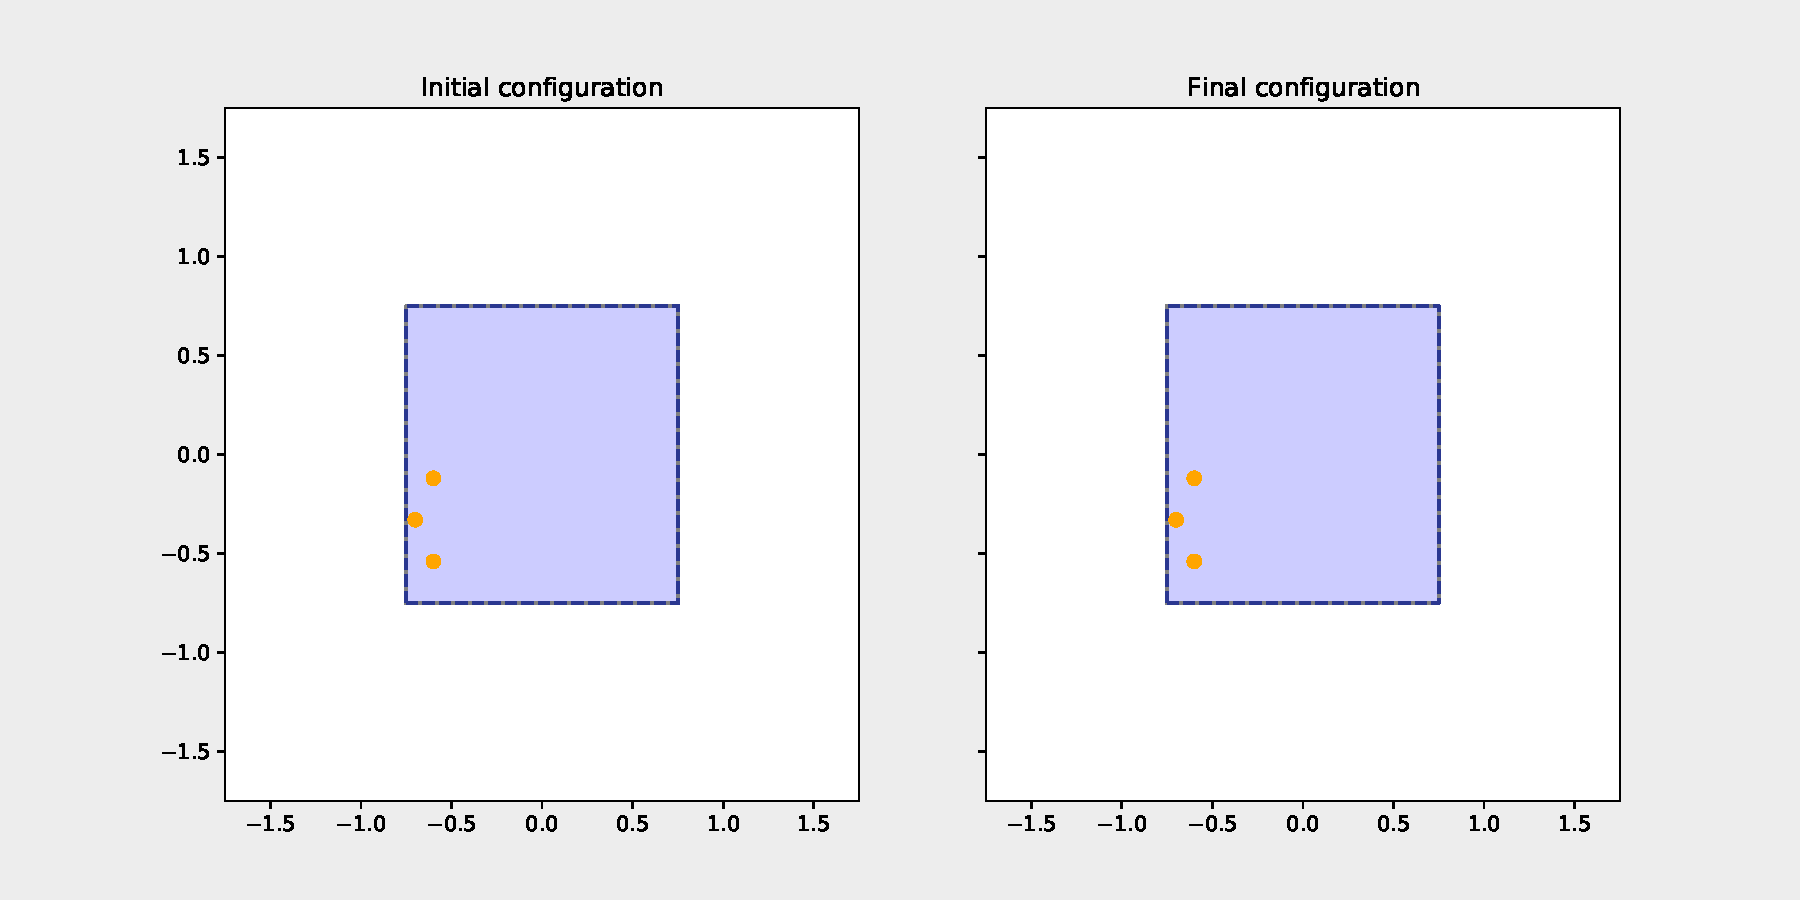
\includegraphics[width=\textwidth]{figs/tinyworld_3_agnt_k_1_0_k_2_1_distr.pdf}
  \caption{Initial and final configuration of 3 agents in the Tinyworld environment with $k_{1} = 0$ (no active dispersion).}
  \label{fig:3_agnt_tw_k_1_0_distr}
\end{figure}

\begin{figure}[H]
  \centering
  \begin{subfigure}[t]{0.5\textwidth}
    \centering
    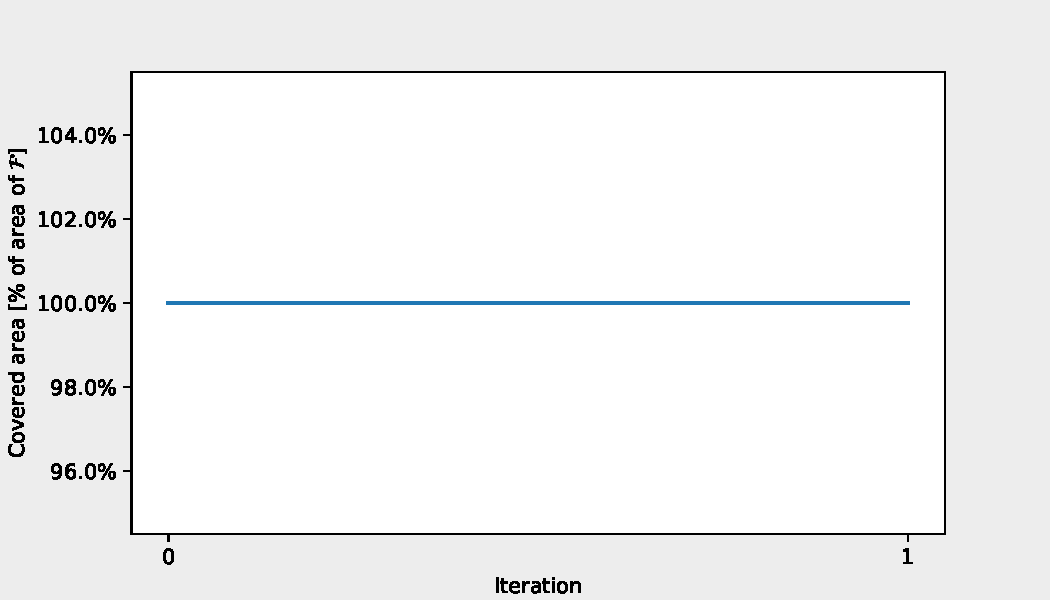
\includegraphics[width=\textwidth]{figs/tinyworld_3_agnt_k_1_0_k_2_1_area_traj.pdf}
    \caption{Coverage evolution for 3 agents in the Tinyworld environment with $k_{1} = 0$ (no active dispersion).}
    \label{fig:3_agnt_tw_k_1_0_a_traj}
  \end{subfigure}%
  ~ 
  \begin{subfigure}[t]{0.5\textwidth}
    \centering
    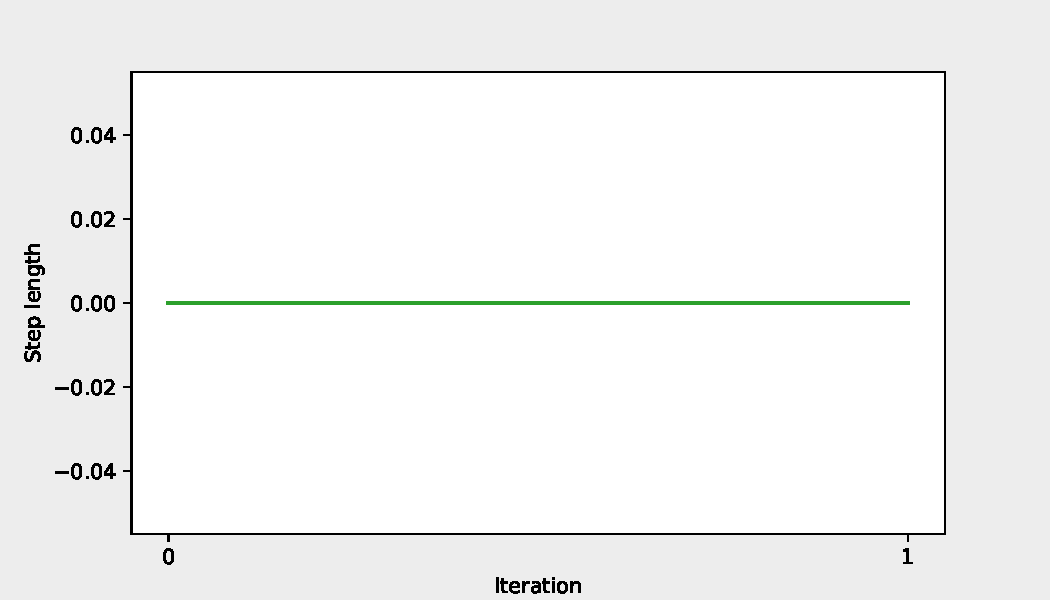
\includegraphics[width=\textwidth]{figs/tinyworld_3_agnt_k_1_0_k_2_1_step_traj.pdf}
    \caption{Step length evolution for 3 agents in the Tinyworld environment with $k_{1} = 0$ (no active dispersion).}
    \label{fig:3_agnt_tw_k_1_0_s_traj}
  \end{subfigure}
  \caption{Coverage percentage and step length evolution for 3 agents in the Tinyworld environment when no active dispersion is used.}
  \label{fig:3_agnt_tw_evolution}
\end{figure}

\begin{figure}[H]
  \centering
  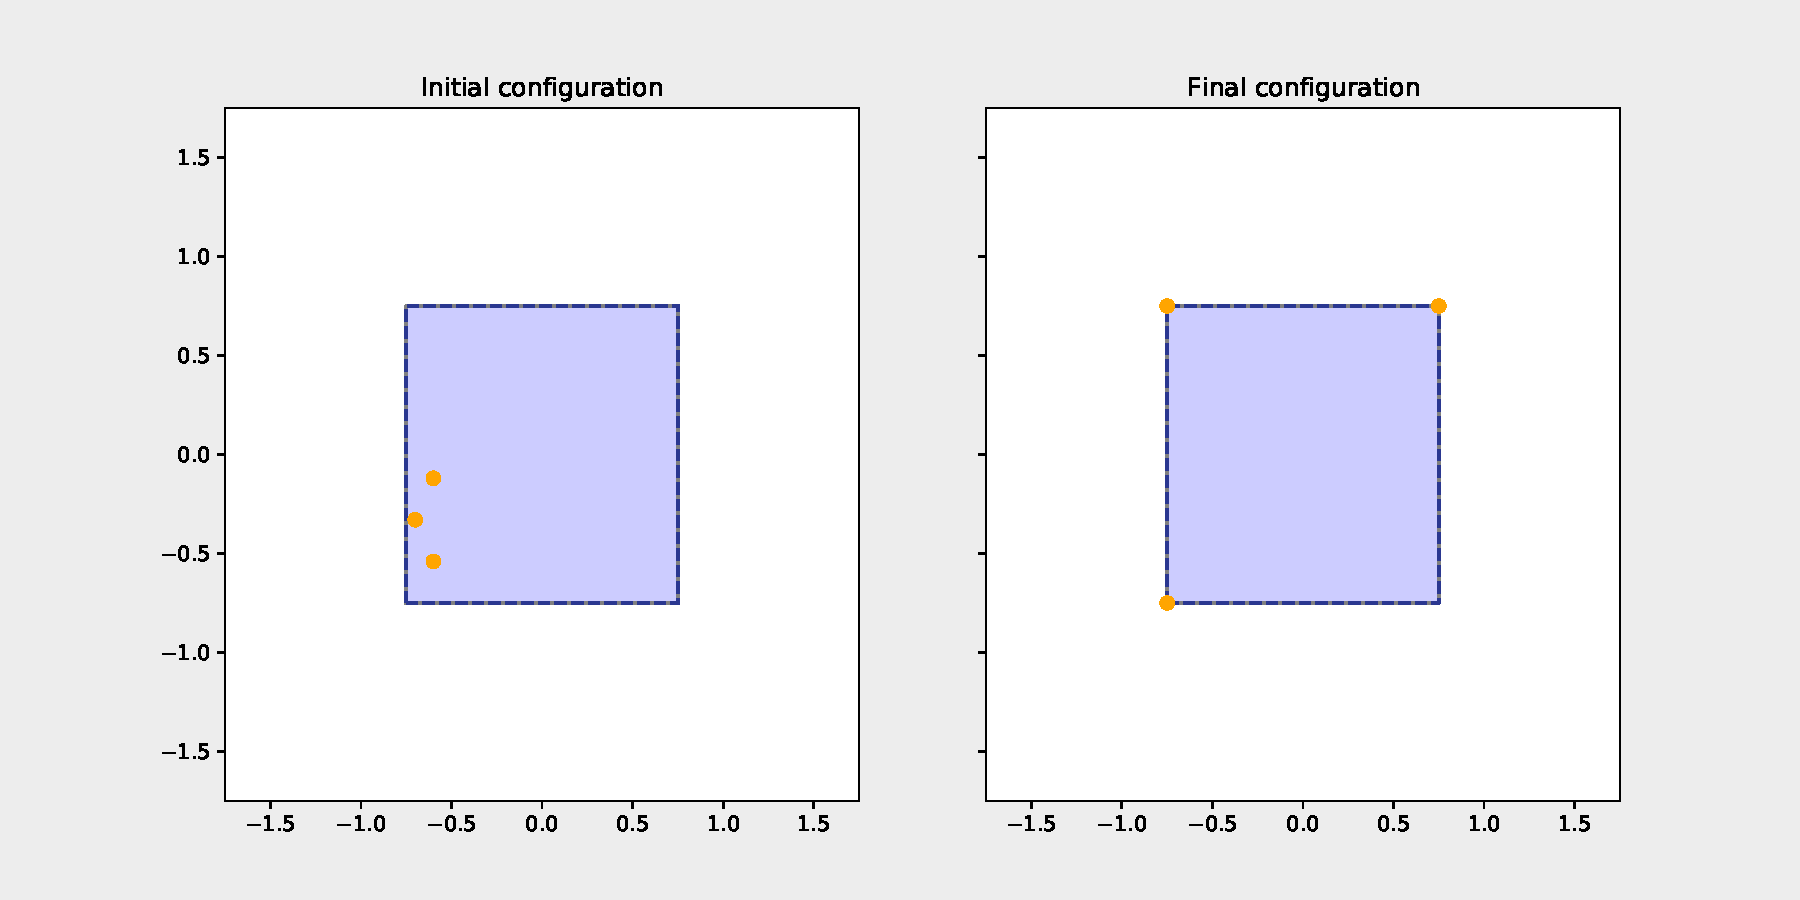
\includegraphics[width=\textwidth]{figs/tinyworld_3_agnt_k_1_1_k_2_1_distr.pdf}
  \caption{Initial and final configuration of 3 agents in the Tinyworld environment with $k_{1} = k_{2} = 1$ (active dispersion).}
  \label{fig:3_agnt_tw_k_1_1_k_2_1_distr}
\end{figure}

\begin{figure}[H]
  \centering
  \begin{subfigure}[t]{0.5\textwidth}
    \centering
    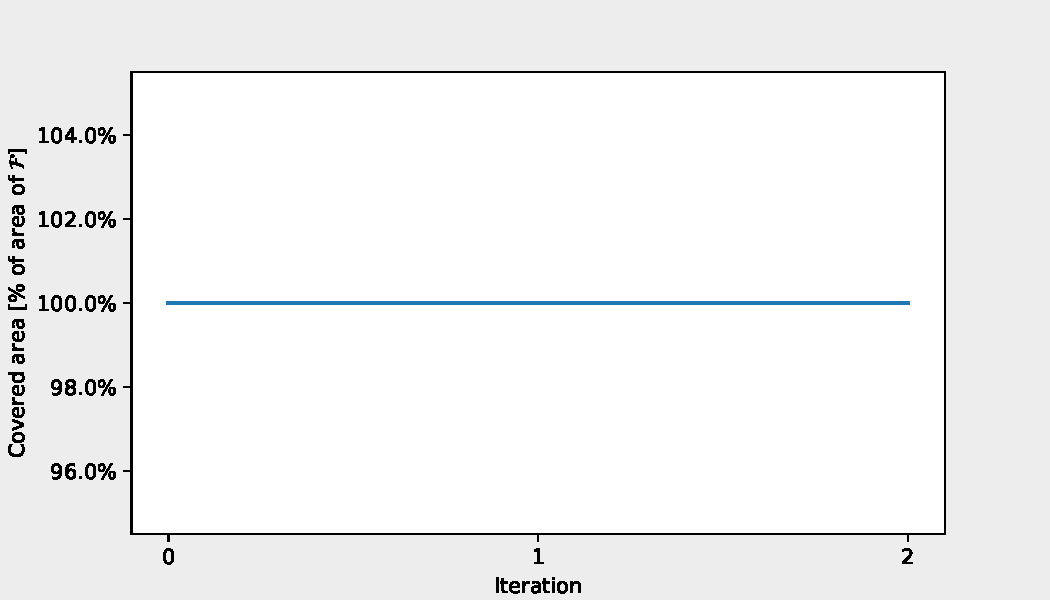
\includegraphics[width=\textwidth]{figs/tinyworld_3_agnt_k_1_1_k_2_1_area_traj.pdf}
    \caption{Coverage evolution for 3 agents in the Tinyworld environment with $k_{1} = k_{2} = 1$ (active dispersion).}
    \label{fig:3_agnt_tw_k_1_k_2_1_a_traj}
  \end{subfigure}%
  ~ 
  \begin{subfigure}[t]{0.5\textwidth}
    \centering
    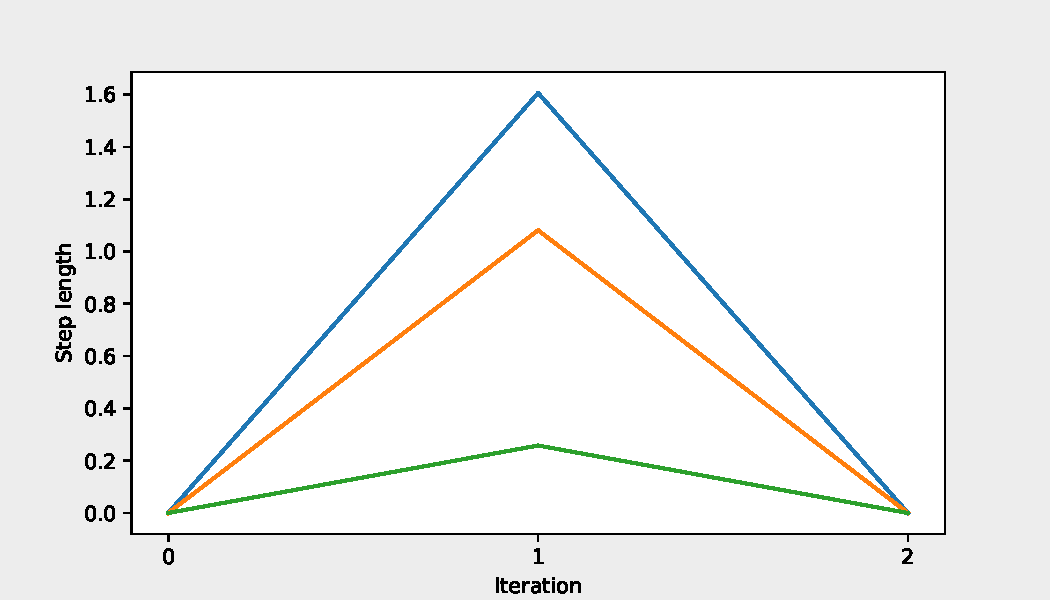
\includegraphics[width=\textwidth]{figs/tinyworld_3_agnt_k_1_1_k_2_1_step_traj.pdf}
    \caption{Step length evolution for 3 agents in the Tinyworld environment with $k_{1} = k_{2} = 1$ (active dispersion).}
    \label{fig:3_agnt_tw_k_1_k_2_1_s_traj}
  \end{subfigure}
  \caption{Coverage percentage and step length evolution for 3 agents in the Tinyworld environment when active dispersion is used.}
  \label{fig:3_agnt_tw_evolution_active}
\end{figure}
\clearpage
\subsection{Tinyworld2}\label[secc]{tinyworld2}
The Tinyworld2 environment is constructed to study how obstacles affect the configuration generated by Algorithm \ref{alg:alg1}.

The results of a simulation for 3 agents without active dispersion ($k_{1} = 0$) is shown in \Crefrange{fig:3_agnt_tw2_k_1_0_distr}{fig:3_agnt_tw2_evolution}.
\Crefrange{fig:6_agnt_tw2_k_1_0_distr}{fig:6_agnt_tw2_evolution} show the results of a simulation of 6 agents without active dispersion.

The results generated by Algorithm \ref{alg:alg1} when applying active dispersion ($k_{1} = 1$, $k_{1} = 2$) and running simulations for 3 and 6 agents 
are shown in \Crefrange{fig:3_agnt_tw2_k_1_1_k_2_1_distr}{fig:3_agnt_tw2_evolution_active} and \Crefrange{fig:6_agnt_tw2_k_1_1_k_2_1_distr}{fig:6_agnt_tw2_evolution_active} respectively.
\begin{figure}[H]
  \centering
  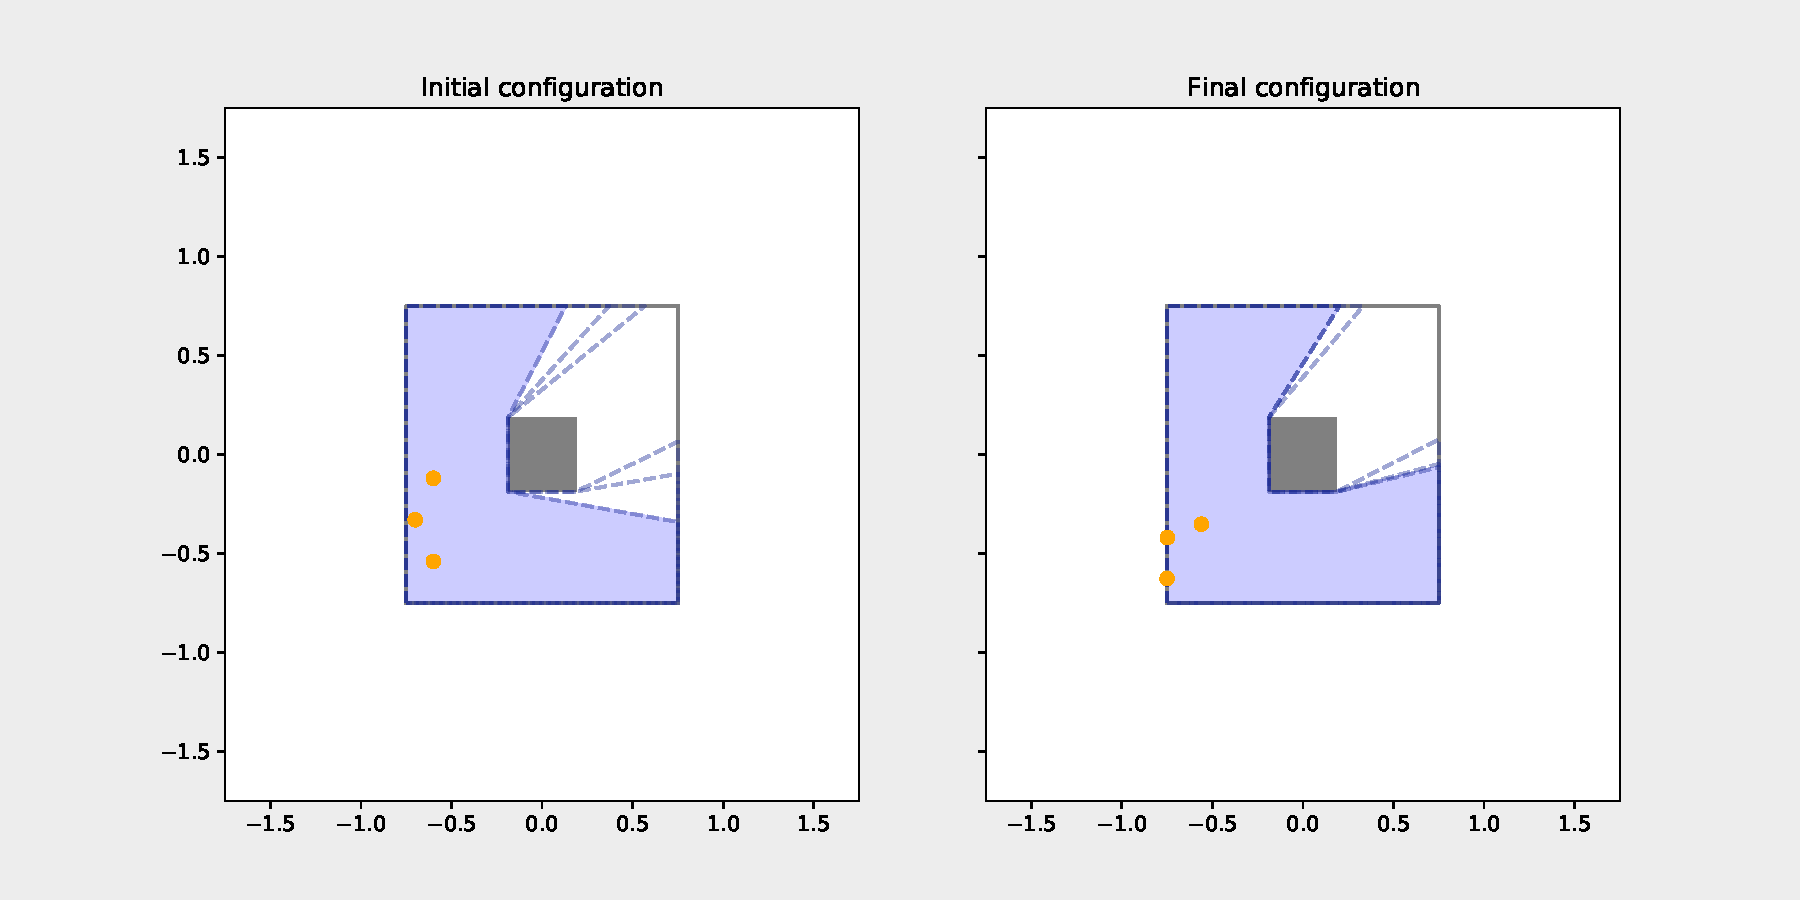
\includegraphics[width=\textwidth]{figs/tinyworld2_3_agnt_k_1_0_k_2_1_distr.pdf}
  \caption{Inital and final configuration of 3 agents in the Tinyworld2 environment with $k_{1} = 0$ (no active dispersion).}
  \label{fig:3_agnt_tw2_k_1_0_distr}
\end{figure}
\begin{figure}[H]
  \centering
  \begin{subfigure}[t]{0.5\textwidth}
    \centering
    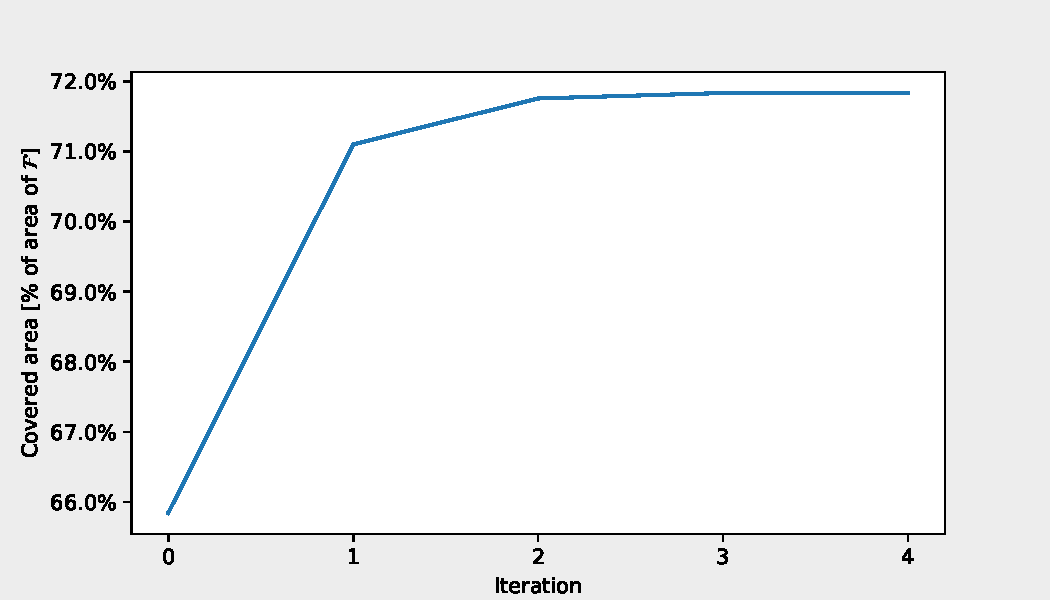
\includegraphics[width=\textwidth]{figs/tinyworld2_3_agnt_k_1_0_k_2_1_area_traj.pdf}
    \caption{Coverage evolution for 3 agents in the Tinyworld2 environment with $k_{1} = 0$ (no active dispersion).}
    \label{fig:3_agnt_tw2_k_1_0_a_traj}
  \end{subfigure}%
  ~ 
  \begin{subfigure}[t]{0.5\textwidth}
    \centering
    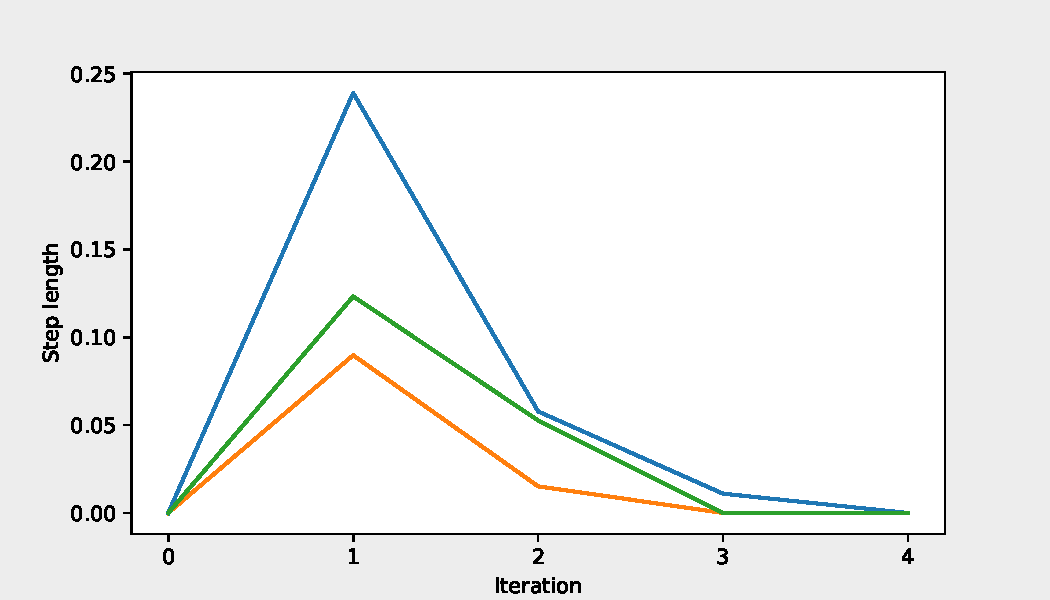
\includegraphics[width=\textwidth]{figs/tinyworld2_3_agnt_k_1_0_k_2_1_step_traj.pdf}
    \caption{Step length evolution for 3 agents in the Tinyworld2 environment with $k_{1} = 0$ (no active dispersion).}
    \label{fig:3_agnt_tw2_k_1_0_s_traj}
  \end{subfigure}
  \caption{Coverage percentage and step length evolution for 3 agents in the Tinyworld2 environment when no active dispersion is used.}
  \label{fig:3_agnt_tw2_evolution}
\end{figure}


\begin{figure}[H]
  \centering
  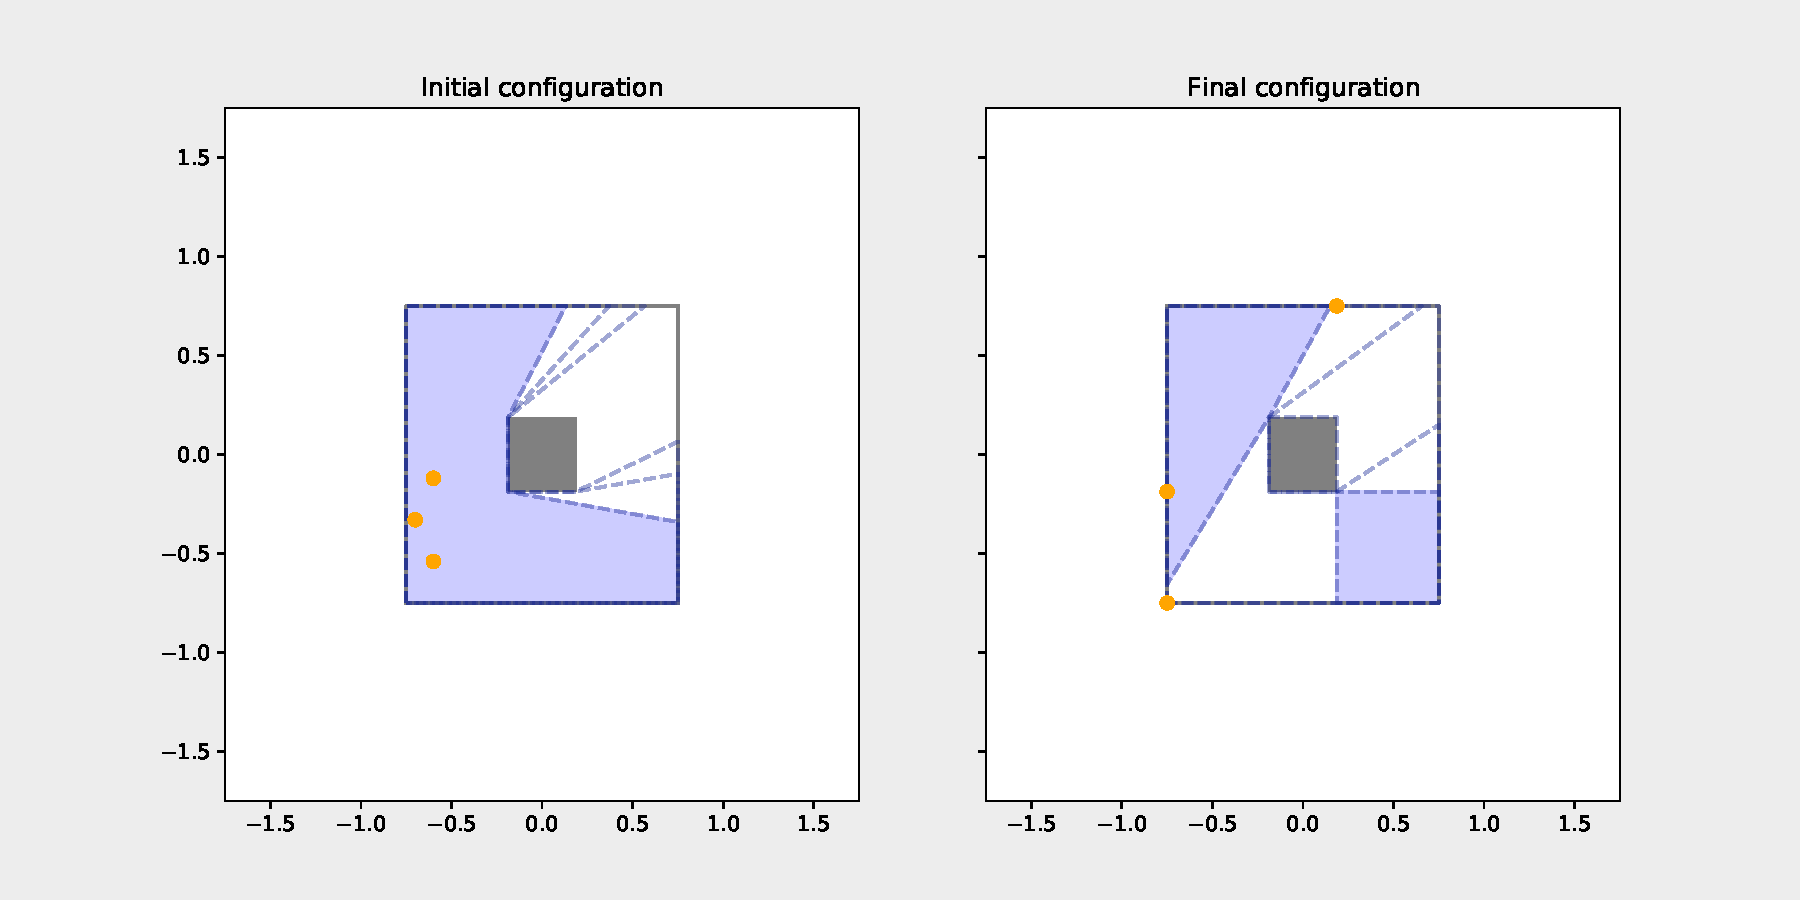
\includegraphics[width=\textwidth]{figs/tinyworld2_3_agnt_k_1_1_k_2_1_distr.pdf}
  \caption{Inital and final configuration of 3 agents in the Tinyworld2 environment with $k_{1} = k_{2} = 1$ (active dispersion).}
  \label{fig:3_agnt_tw2_k_1_1_k_2_1_distr}
\end{figure}
\begin{figure}[H]
  \centering
  \begin{subfigure}[t]{0.5\textwidth}
    \centering
    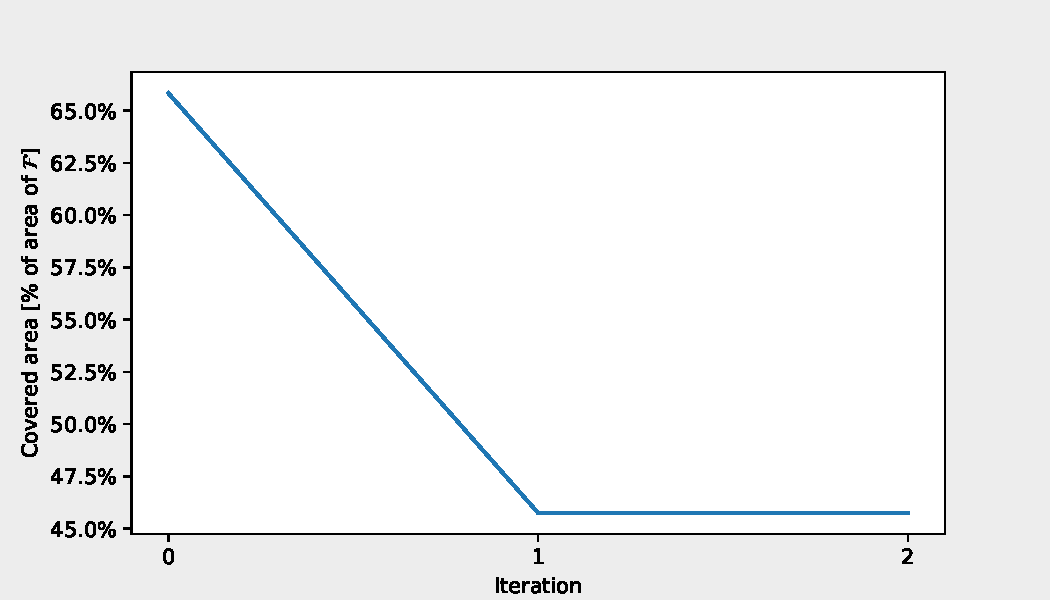
\includegraphics[width=\textwidth]{figs/tinyworld2_3_agnt_k_1_1_k_2_1_area_traj.pdf}
    \caption{Coverage evolution for 3 agents in the Tinyworld2 environment with $k_{1} = k_{2} = 1$ (active dispersion).}
    \label{fig:3_agnt_tw2_k_1_1_a_traj}
  \end{subfigure}%
  ~ 
  \begin{subfigure}[t]{0.5\textwidth}
    \centering
    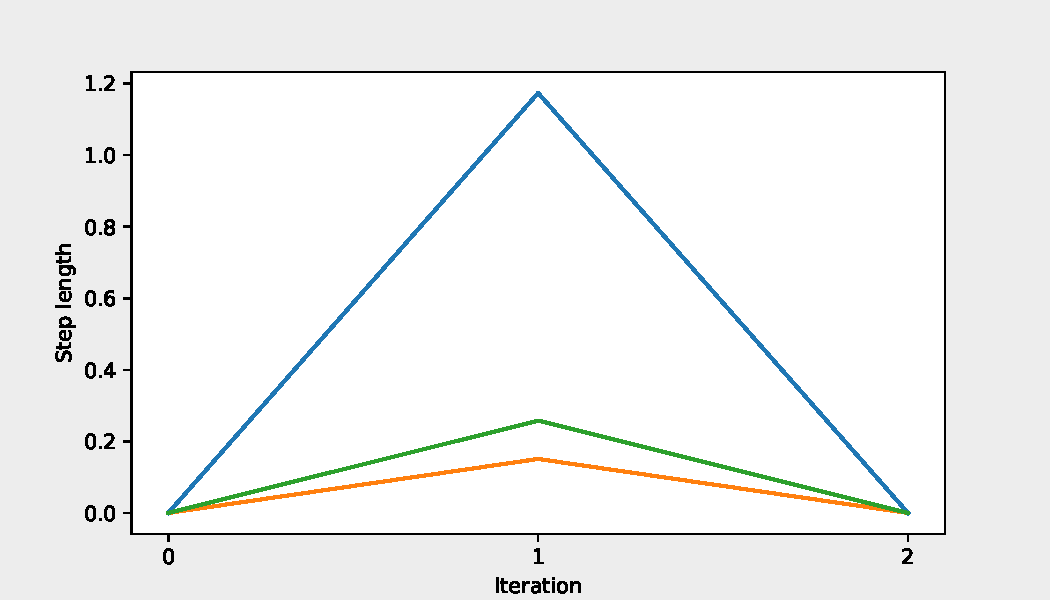
\includegraphics[width=\textwidth]{figs/tinyworld2_3_agnt_k_1_1_k_2_1_step_traj.pdf}
    \caption{Step length evolution for 3 agents in the Tinyworld2 environment with $k_{1} = k_{2} = 1$ (active dispersion).}
    \label{fig:3_agnt_tw2_k_1_1_s_traj}
  \end{subfigure}
  \caption{Coverage percentage and step length evolution for 3 agents in the Tinyworld2 environment when active dispersion is used.}
  \label{fig:3_agnt_tw2_evolution_active}
\end{figure}

\begin{figure}[H]
  \centering
  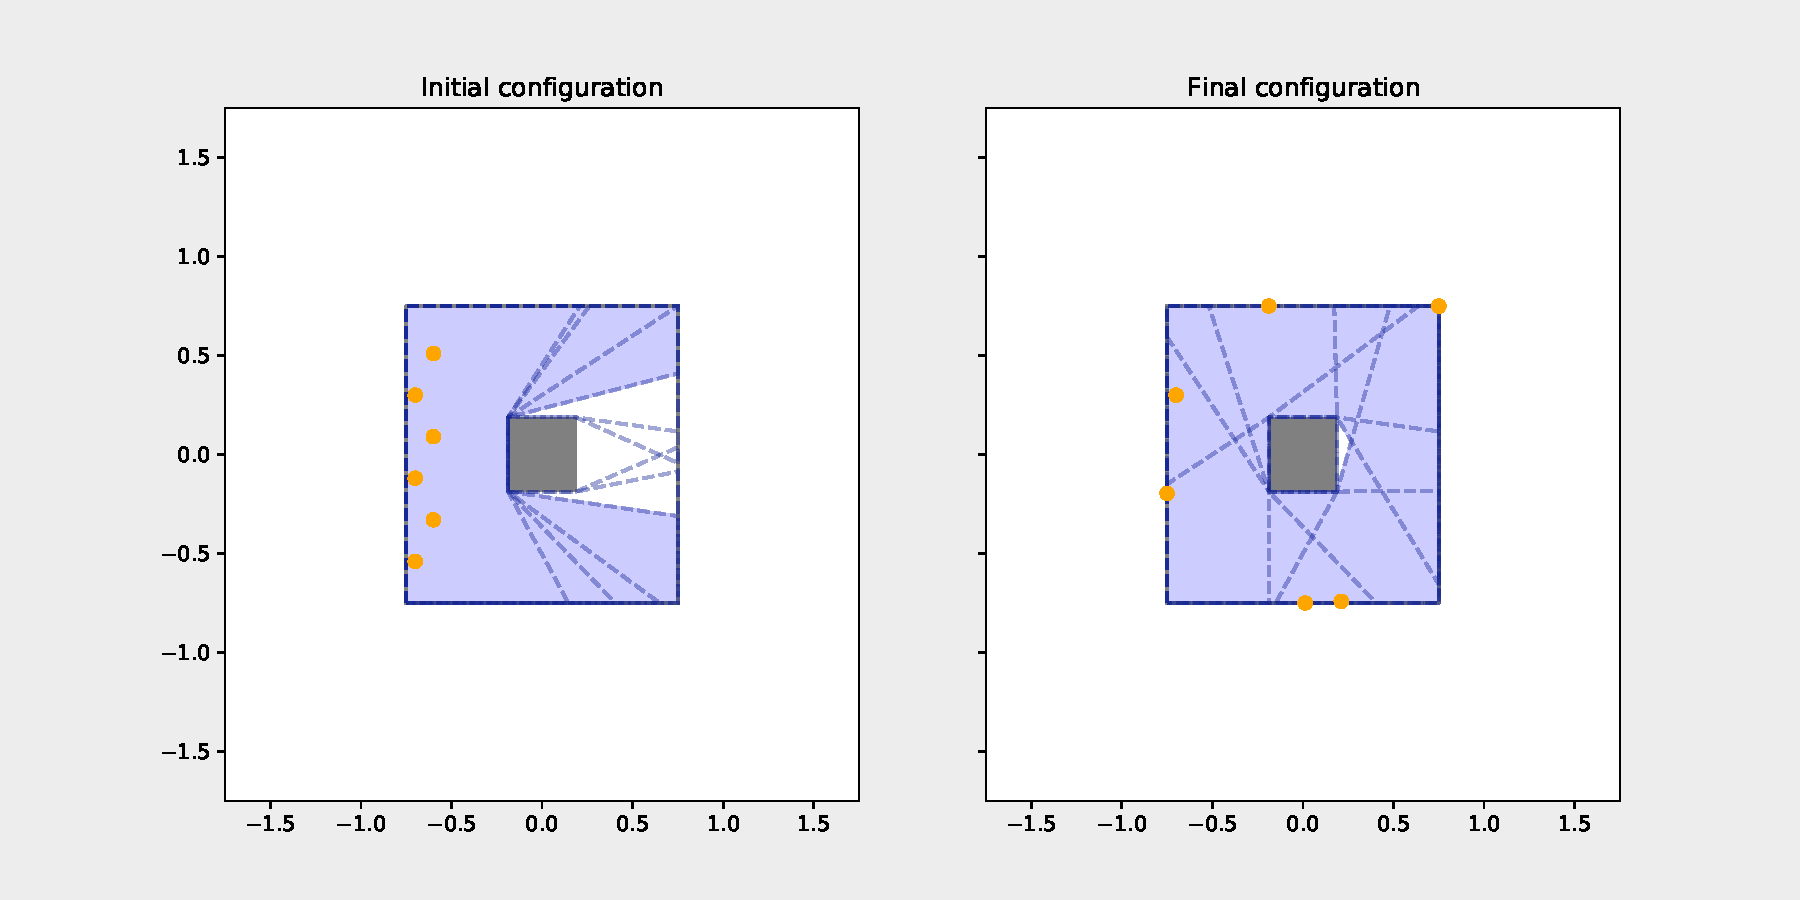
\includegraphics[width=\textwidth]{figs/tinyworld2_6_agnt_k_1_0_k_2_1_distr.pdf}
  \caption{Inital and final configuration of 6 agents in the Tinyworld2 environment with $k_{1} = 0$ (no active dispersion).}
  \label{fig:6_agnt_tw2_k_1_0_distr}
\end{figure}
\begin{figure}[H]
  \centering
  \begin{subfigure}[t]{0.5\textwidth}
    \centering
    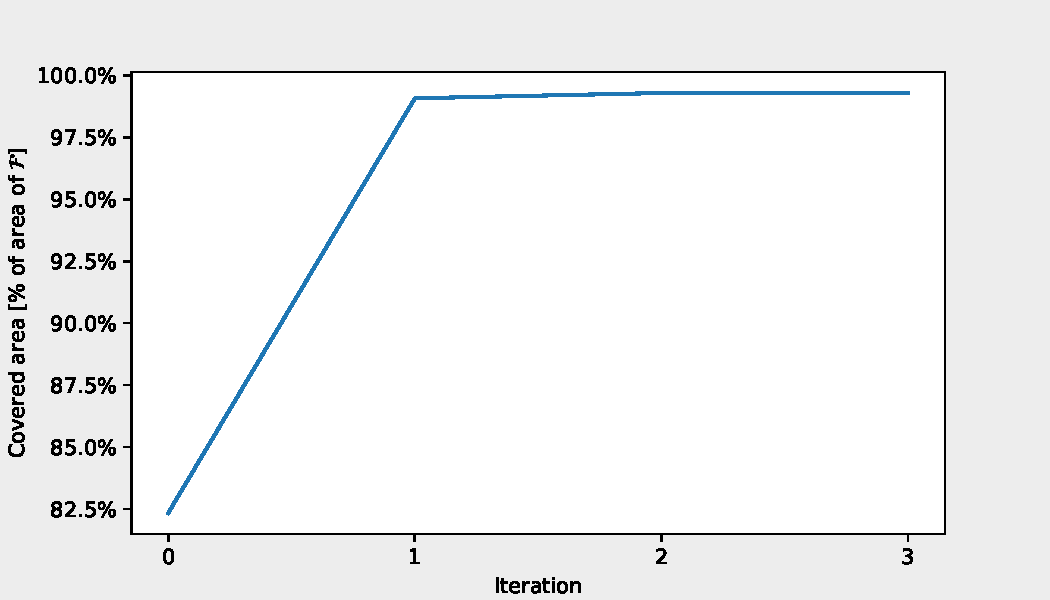
\includegraphics[width=\textwidth]{figs/tinyworld2_6_agnt_k_1_0_k_2_1_area_traj.pdf}
    \caption{Coverage evolution for 6 agents in the Tinyworld2 environment with $k_{1} = 0$ (no active dispersion).}
    \label{fig:6_agnt_tw2_k_1_0_a_traj}
  \end{subfigure}%
  ~ 
  \begin{subfigure}[t]{0.5\textwidth}
    \centering
    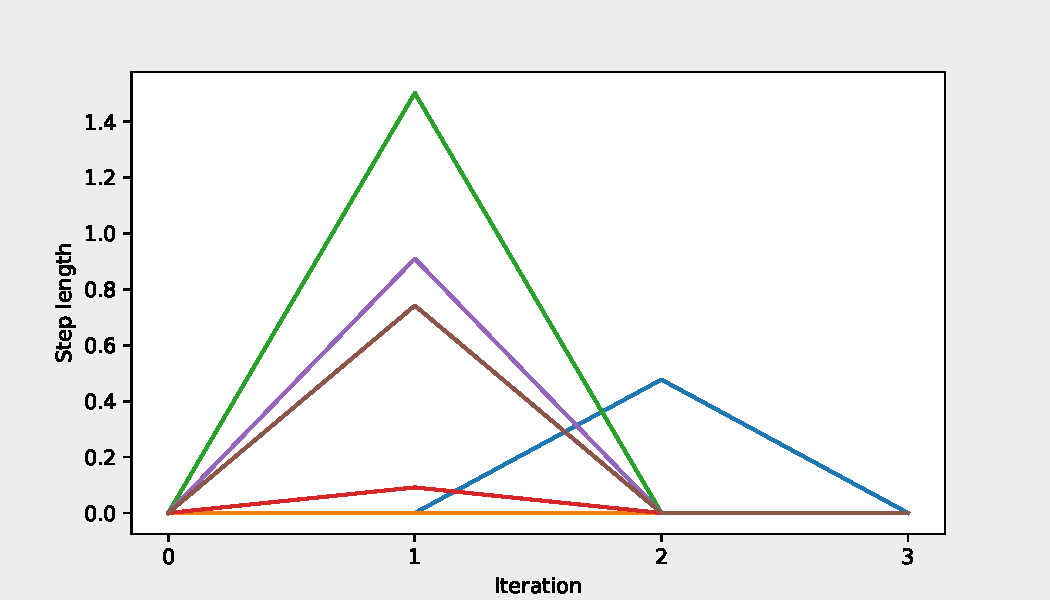
\includegraphics[width=\textwidth]{figs/tinyworld2_6_agnt_k_1_0_k_2_1_step_traj.pdf}
    \caption{Step length evolution for 6 agents in the Tinyworld2 environment with $k_{1} = 0$ (no active dispersion).}
    \label{fig:6_agnt_tw2_k_1_0_s_traj}
  \end{subfigure}
  \caption{Coverage percentage and step length evolution for 6 agents in the Tinyworld2 environment when active dispersion is not applied.}
  \label{fig:6_agnt_tw2_evolution}
\end{figure}

\begin{figure}[H]
  \centering
  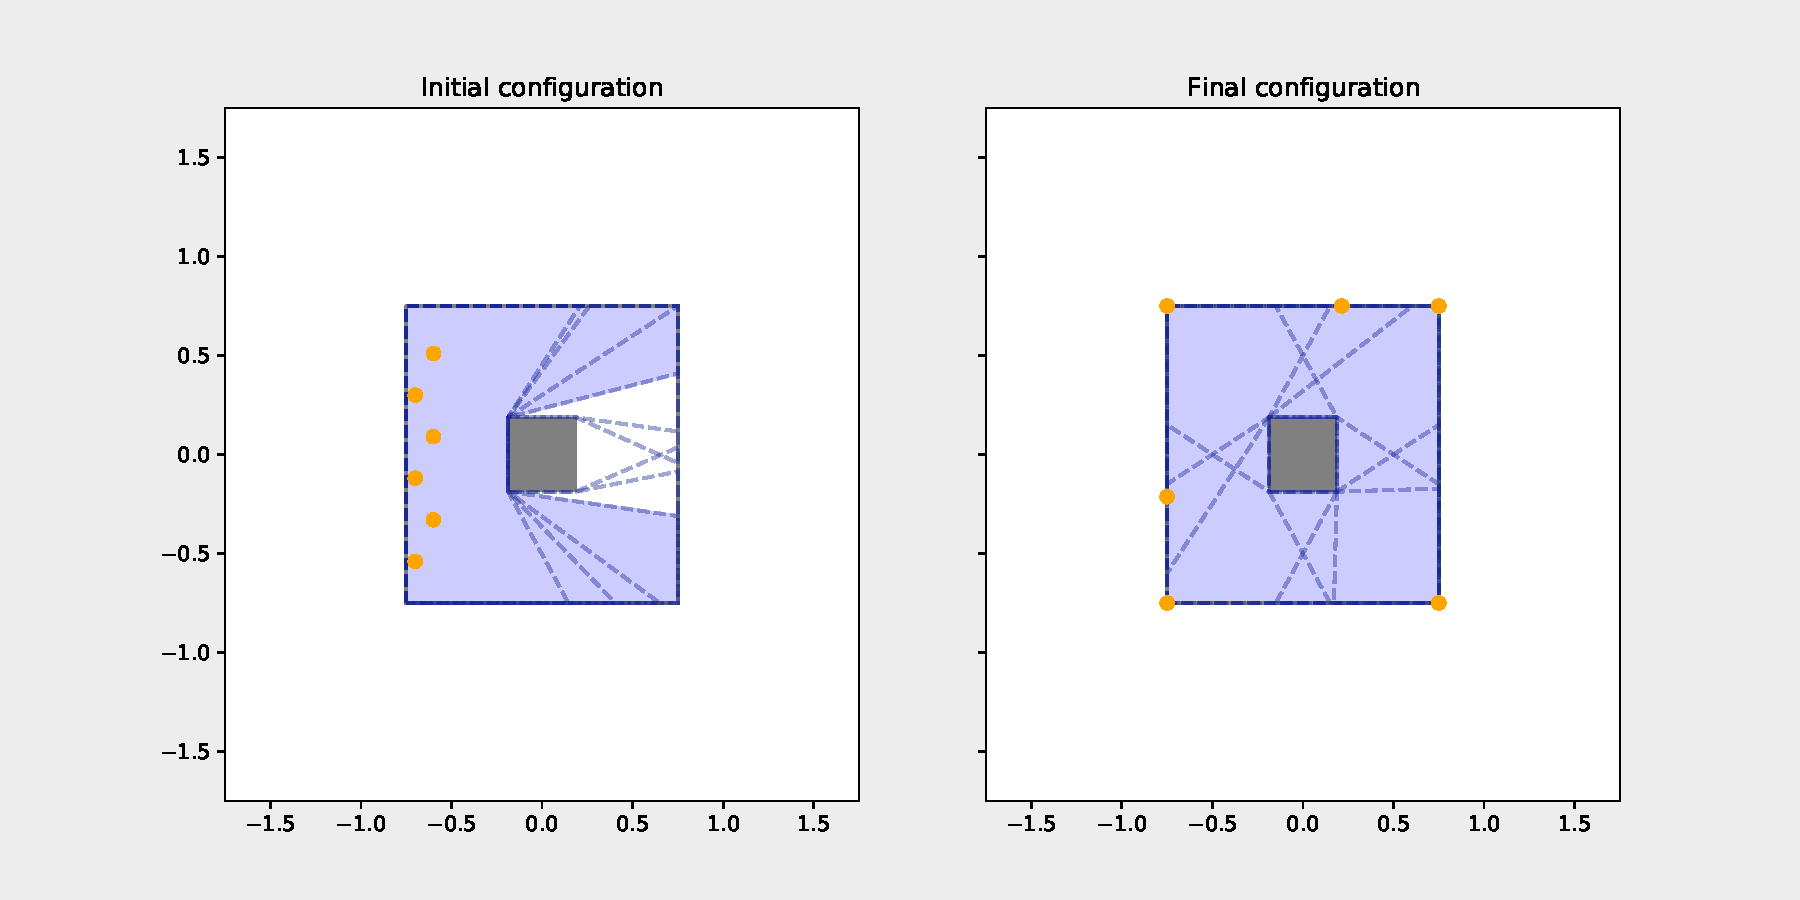
\includegraphics[width=\textwidth]{figs/tinyworld2_6_agnt_k_1_1_k_2_1_distr.pdf}
  \caption{Inital and final configuration of 6 agents in the Tinyworld2 environment with $k_{1} = k_{2} = 1$ (active dispersion).}
  \label{fig:6_agnt_tw2_k_1_1_k_2_1_distr}
\end{figure}
\begin{figure}[H]
  \centering
  \begin{subfigure}[t]{0.5\textwidth}
    \centering
    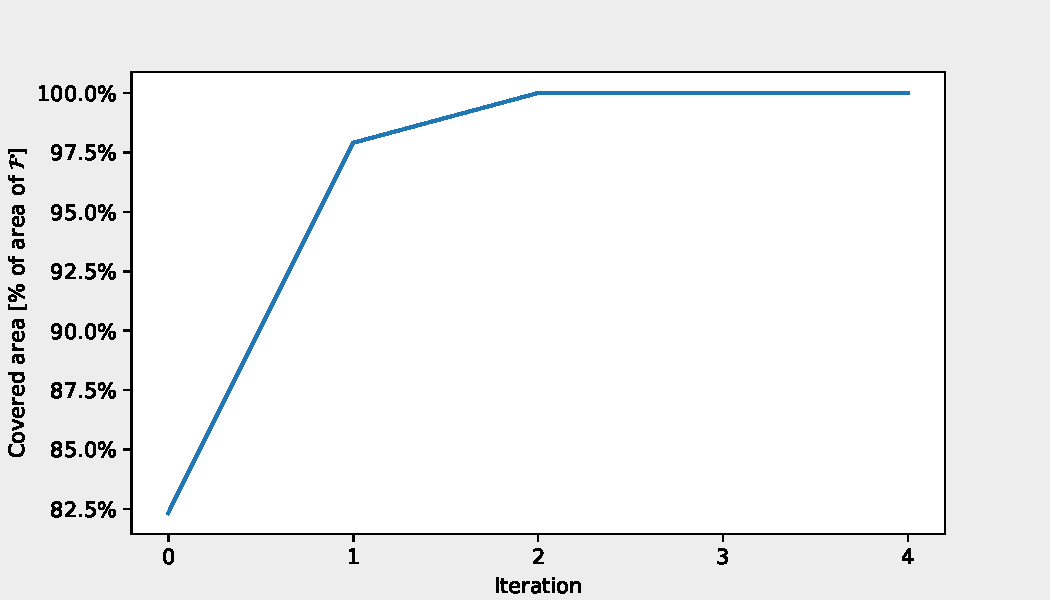
\includegraphics[width=\textwidth]{figs/tinyworld2_6_agnt_k_1_1_k_2_1_area_traj.pdf}
    \caption{Coverage evolution for 6 agents in the Tinyworld2 environment with $k_{1} = k_{1} = 1$ (active dispersion).}
    \label{fig:6_agnt_tw2_k_1_1_a_traj}
  \end{subfigure}%
  ~ 
  \begin{subfigure}[t]{0.5\textwidth}
    \centering
    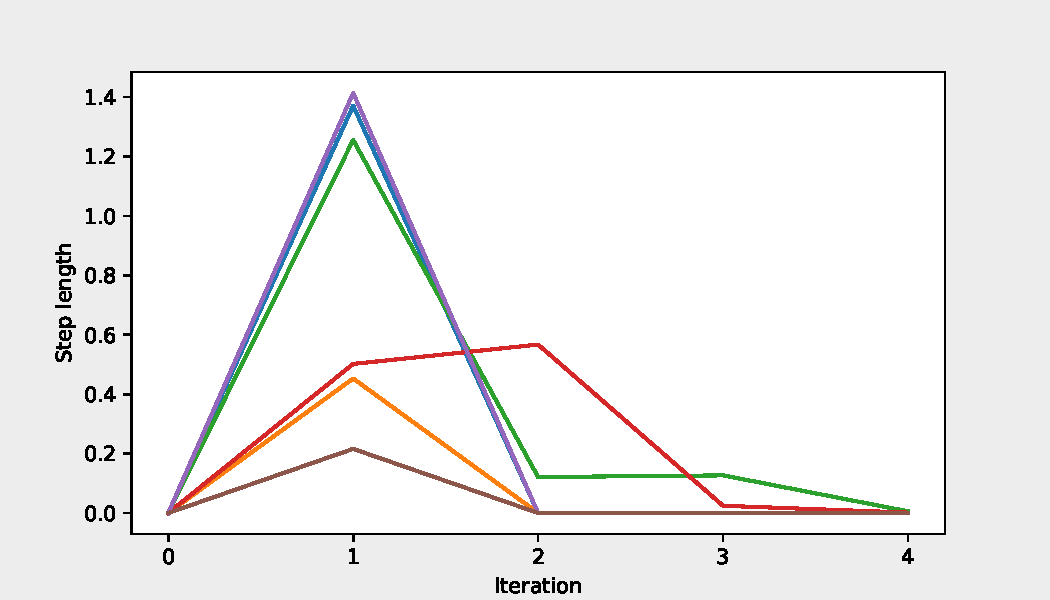
\includegraphics[width=\textwidth]{figs/tinyworld2_6_agnt_k_1_1_k_2_1_step_traj.pdf}
    \caption{Step length evolution for 6 agents in the Tinyworld2 environment with $k_{1} = k_{2} = 1$ (active dispersion).}
    \label{fig:6_agnt_tw2_k_1_1_s_traj}
  \end{subfigure}
  \caption{Coverage percentage and step length evolution for 6 agents in the Tinyworld2 environment when active dispersion is applied.}
  \label{fig:6_agnt_tw2_evolution_active}
\end{figure}

\clearpage
\subsection{Rectworld}\label[secc]{rectworld}
The Rectworld is constructed to examine the behavior of Algorithm \ref{alg:alg1} for a larger mission space. Simulations are performed
for swarms of 3, 6 and 15 agents.

%\Crefrange{fig:3_agnt_bw_k_1_0_k_2_1_distr}{fig:3_agnt_bw_evolution}, \Crefrange{fig:6_agnt_bw_k_1_0_k_2_1_distr}{fig:6_agnt_bw_evolution}
%and \Crefrange{fig:15_agnt_bw_k_1_0_k_2_1_distr}{fig:15_agnt_bw_evolution} show the results of simulating without active dispersion ($k_{1} = 0$) for 3, 6 and 15
%agents respectively.
%
%\Crefrange{fig:3_agnt_bw_k_1_1_k_2_1_distr}{fig:3_agnt_bw_evolution_active}, \Crefrange{fig:6_agnt_bw_k_1_1_k_2_1_distr}{fig:6_agnt_bw_evolution_active}
%and \Crefrange{fig:15_agnt_bw_k_1_1_k_2_1_distr}{fig:15_agnt_bw_evolution_active} show the results of simulating with active dispersion ($k_{1} = k_{2} = 1$) for 3, 6 and 15
%agents respectively.

\begin{figure}[H]
  \centering
  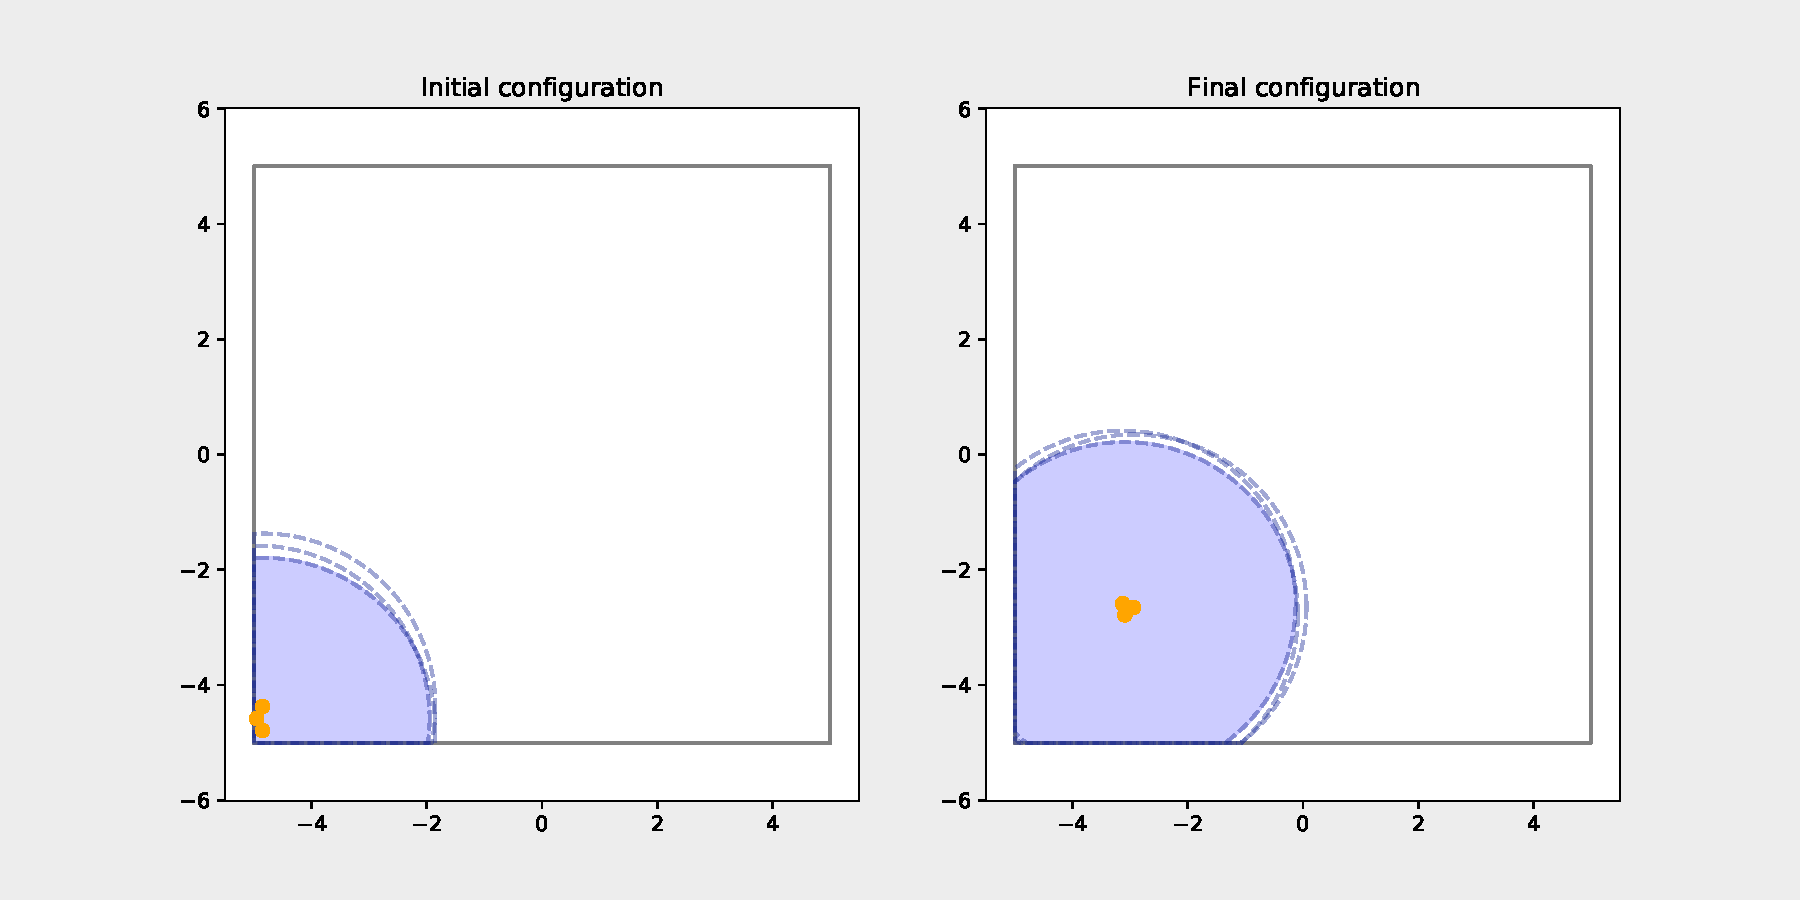
\includegraphics[width=\textwidth]{figs/bigworld_3_agnt_k_1_0_k_2_1_distr.pdf}
  \caption{Initial and final configuration of 3 agents in the Rectworld environment with $k_{1} = 0$ (no active dispersion).}
  \label{fig:3_agnt_bw_k_1_0_k_2_1_distr}
\end{figure}
\begin{figure}[H]
  \centering
  \begin{subfigure}[t]{0.5\textwidth}
    \centering
    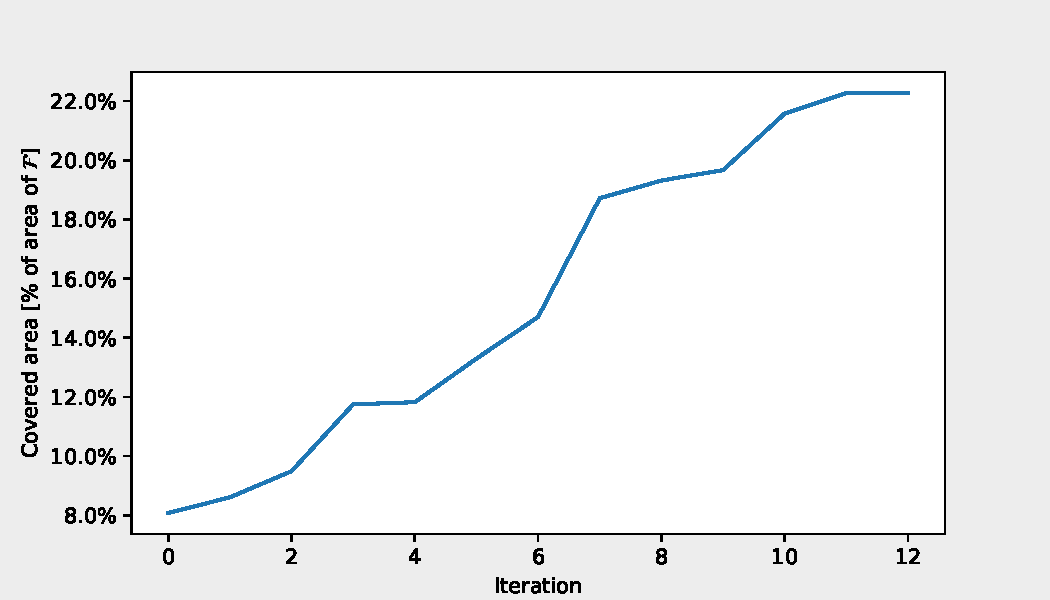
\includegraphics[width=\textwidth]{figs/bigworld_3_agnt_k_1_0_k_2_1_area_traj.pdf}
    \caption{Coverage evolution for 3 agents in the Rectworld environment with $k_{1} = 0$ (no active dispersion).}
    \label{fig:3_agnt_bw_k_1_0_a_traj}
  \end{subfigure}%
  ~ 
  \begin{subfigure}[t]{0.5\textwidth}
    \centering
    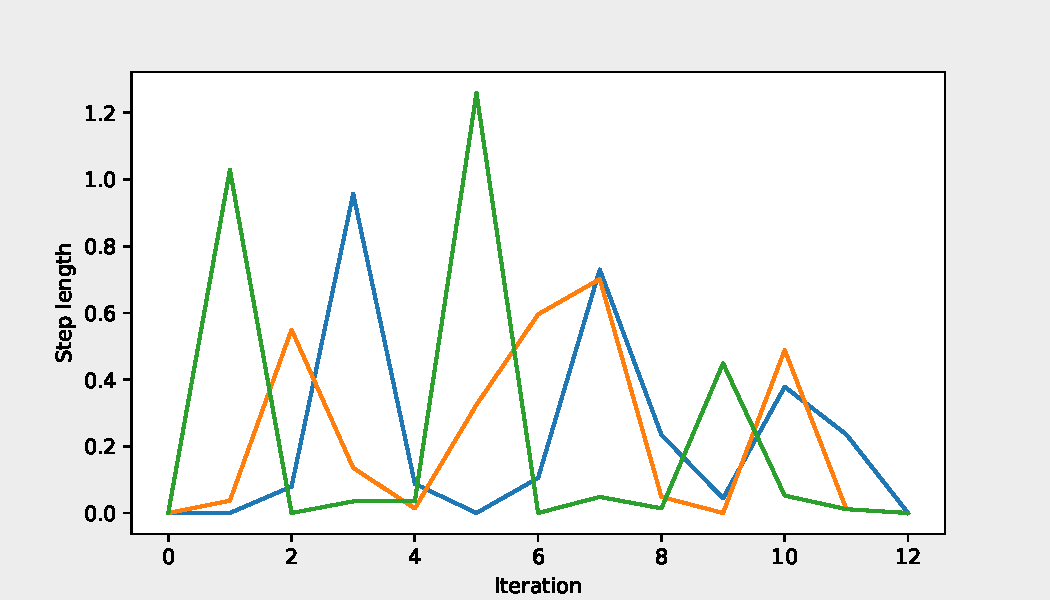
\includegraphics[width=\textwidth]{figs/bigworld_3_agnt_k_1_0_k_2_1_step_traj.pdf}
    \caption{Step length evolution for 3 agents in the Rectworld environment with $k_{1} = 0$ (no active dispersion).}
    \label{fig:3_agnt_bw_k_1_0_s_traj}
  \end{subfigure}
  \caption{Coverage percentage and step length evolution for 3 agents in the Rectworld environment when no active dispersion is used.}
  \label{fig:3_agnt_bw_evolution}
\end{figure}


\begin{figure}[H]
  \centering
  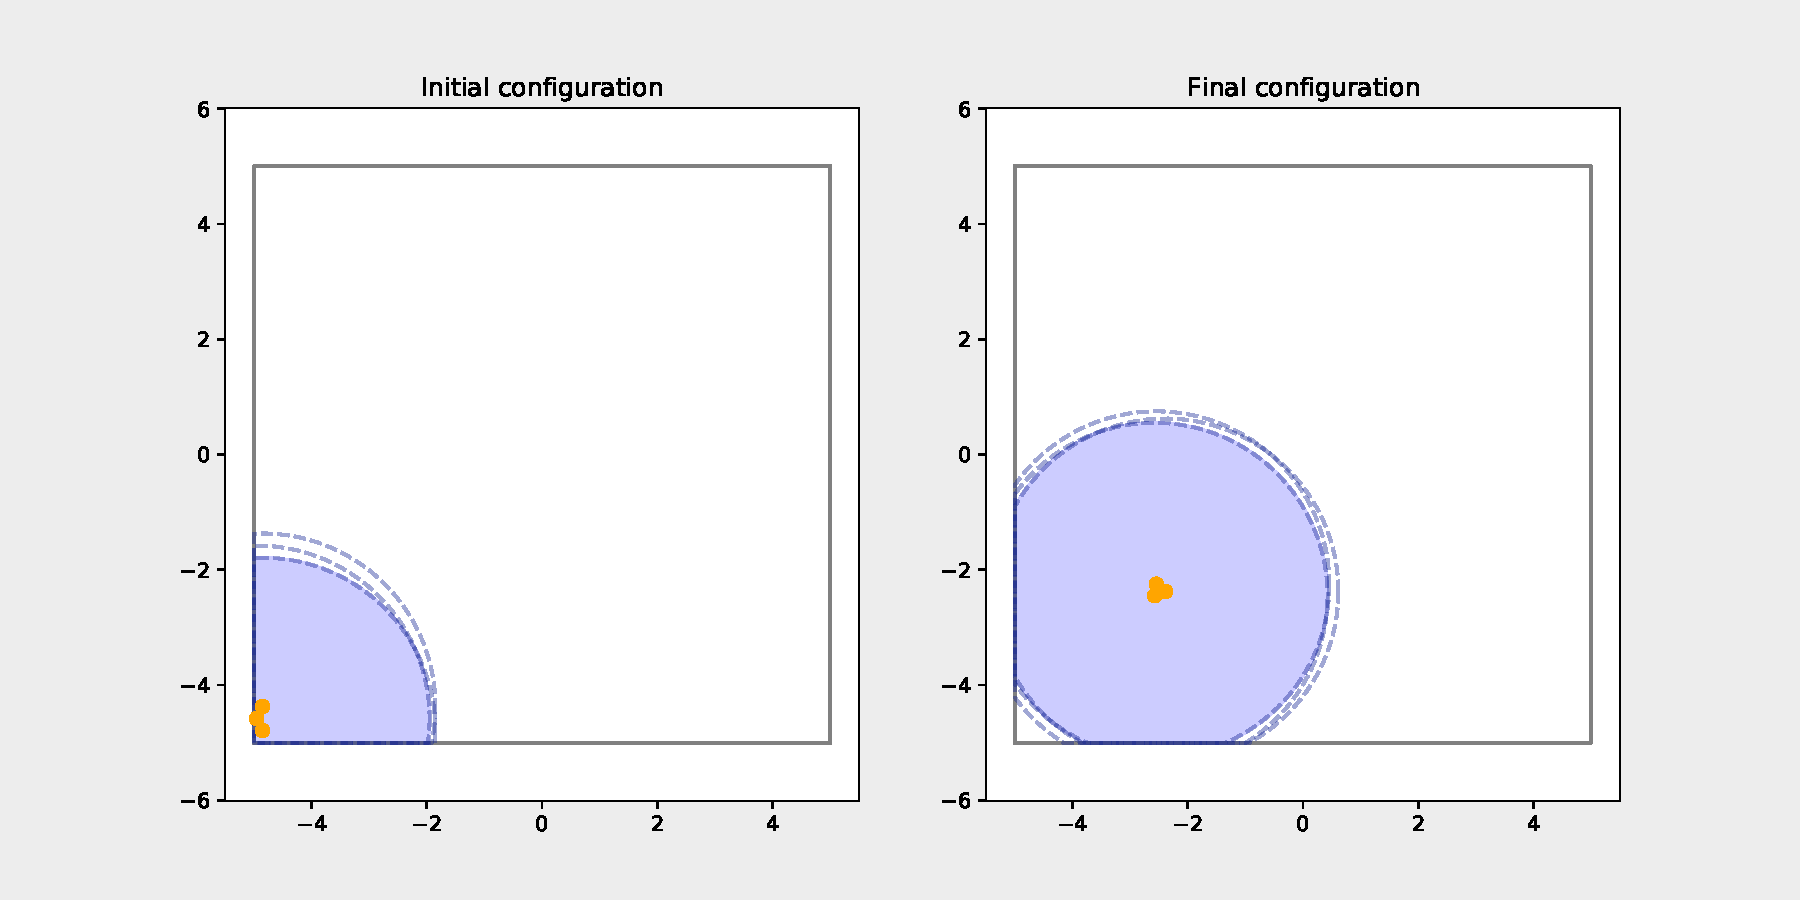
\includegraphics[width=\textwidth]{figs/bigworld_3_agnt_k_1_1_k_2_1_distr.pdf}
  \caption{Initial and final configuration of 3 agents in the Rectworld environment with $k_{1} = k_{2} = 1$ (active dispersion).}
  \label{fig:3_agnt_bw_k_1_1_k_2_1_distr}
\end{figure}
\begin{figure}[H]
  \centering
  \begin{subfigure}[t]{0.5\textwidth}
    \centering
    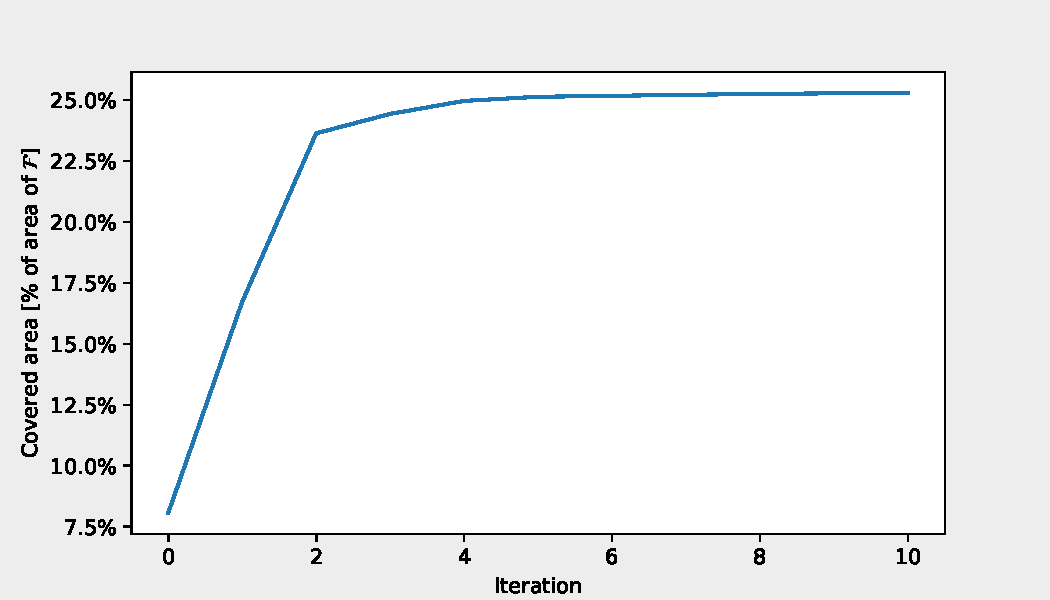
\includegraphics[width=\textwidth]{figs/bigworld_3_agnt_k_1_1_k_2_1_area_traj.pdf}
    \caption{Coverage evolution for 3 agents in the Rectworld environment with $k_{1} = k_{1} = 1$ (active dispersion).}
    \label{fig:3_agnt_bw_k_1_1_a_traj}
  \end{subfigure}%
  ~ 
  \begin{subfigure}[t]{0.5\textwidth}
    \centering
    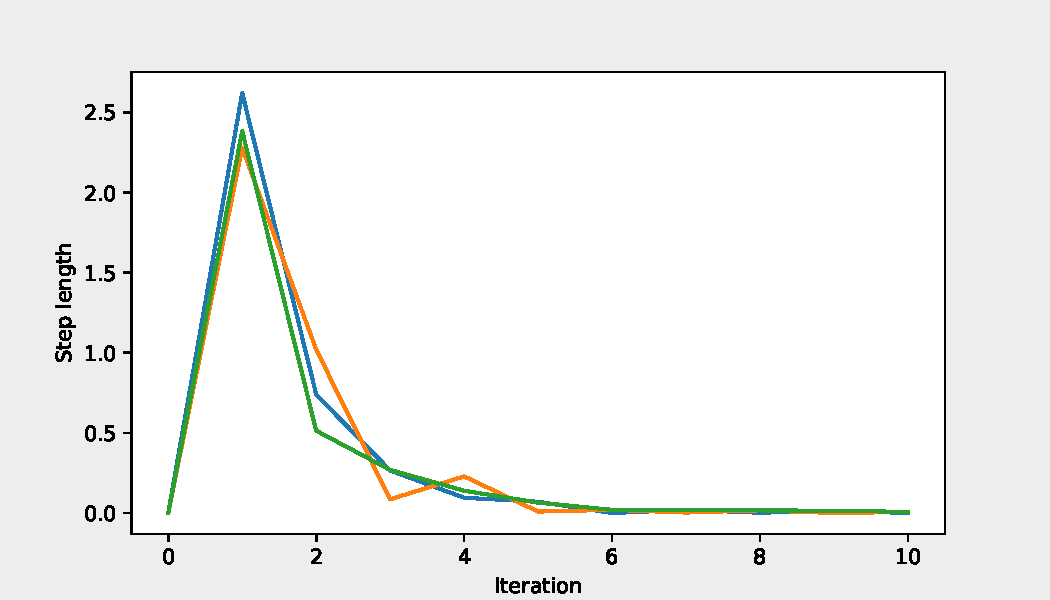
\includegraphics[width=\textwidth]{figs/bigworld_3_agnt_k_1_1_k_2_1_step_traj.pdf}
    \caption{Step length evolution for 3 agents in the Rectworld environment with $k_{1} = k_{1} = 1$ (active dispersion).}
    \label{fig:3_agnt_bw_k_1_1_s_traj}
  \end{subfigure}
  \caption{Coverage percentage and step length evolution for 3 agents in the Rectworld environment when active dispersion is used.}
  \label{fig:3_agnt_bw_evolution_active}
\end{figure}

%%%

\begin{figure}[H]
  \centering
  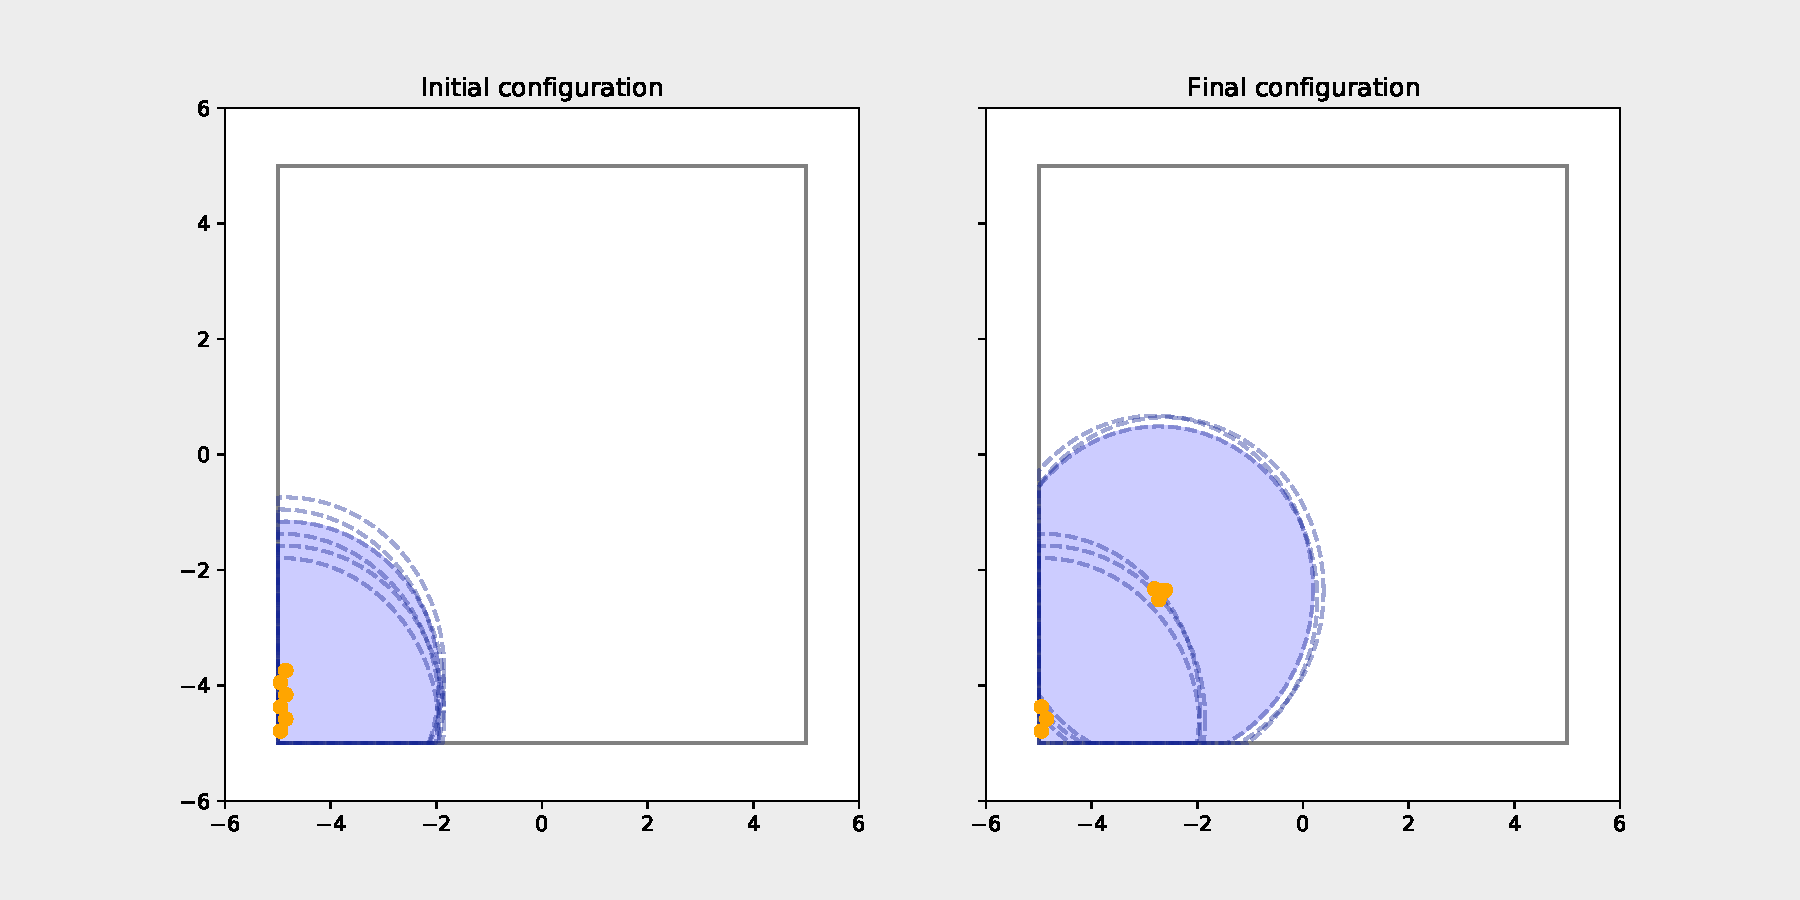
\includegraphics[width=\textwidth]{figs/bigworld_6_agnt_k_1_0_k_2_1_distr.pdf}
  \caption{Initial and final configuration of 6 agents in the Rectworld environment with $k_{1} = 0$ (no active dispersion).}
  \label{fig:6_agnt_bw_k_1_0_k_2_1_distr}
\end{figure}
\begin{figure}[H]
  \centering
  \begin{subfigure}[t]{0.5\textwidth}
    \centering
    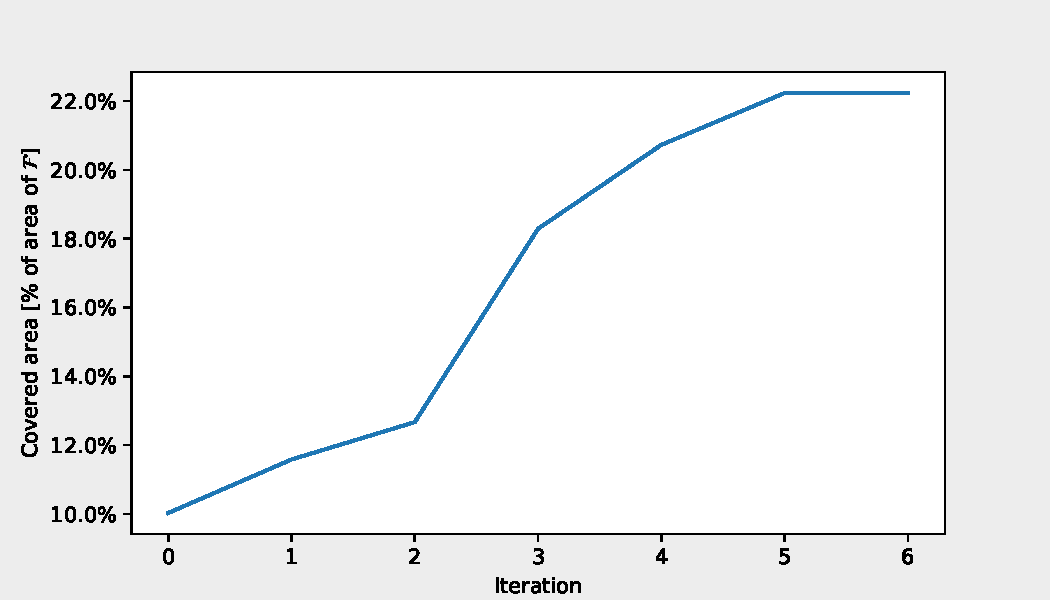
\includegraphics[width=\textwidth]{figs/bigworld_6_agnt_k_1_0_k_2_1_area_traj.pdf}
    \caption{Coverage evolution for 6 agents in the Rectworld environment with $k_{1} = 0$ (no active dispersion).}
    \label{fig:6_agnt_bw_k_1_0_a_traj}
  \end{subfigure}%
  ~ 
  \begin{subfigure}[t]{0.5\textwidth}
    \centering
    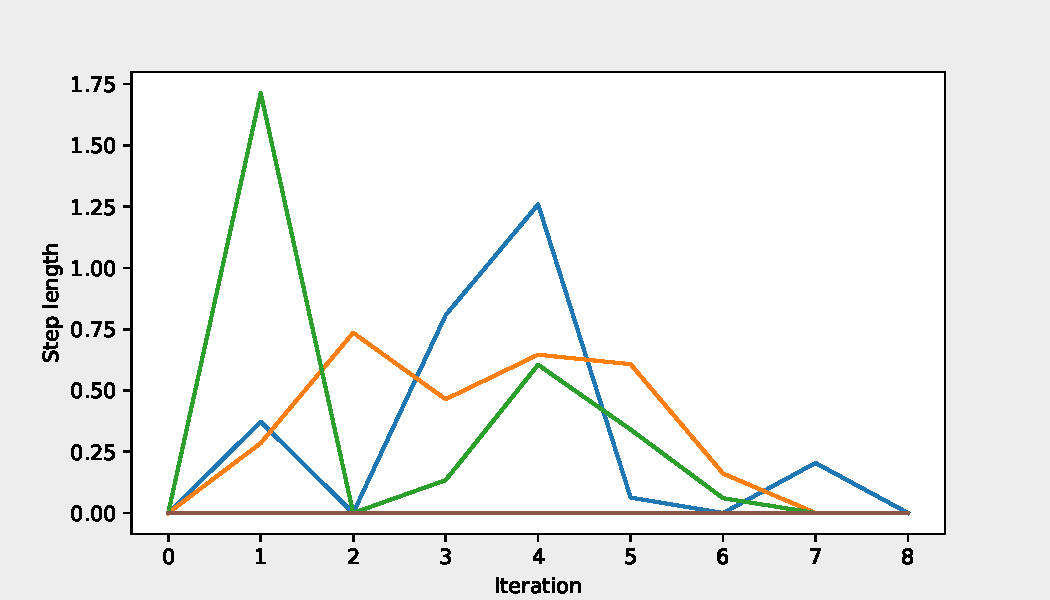
\includegraphics[width=\textwidth]{figs/bigworld_6_agnt_k_1_0_k_2_1_step_traj.pdf}
    \caption{Step length evolution for 6 agents in the Rectworld environment with $k_{1} = 0$ (no active dispersion).}
    \label{fig:6_agnt_bw_k_1_0_s_traj}
  \end{subfigure}
  \caption{Coverage percentage and step length evolution for 6 agents in the Rectworld environment when no active dispersion is used.}
  \label{fig:6_agnt_bw_evolution}
\end{figure}


\begin{figure}[H]
  \centering
  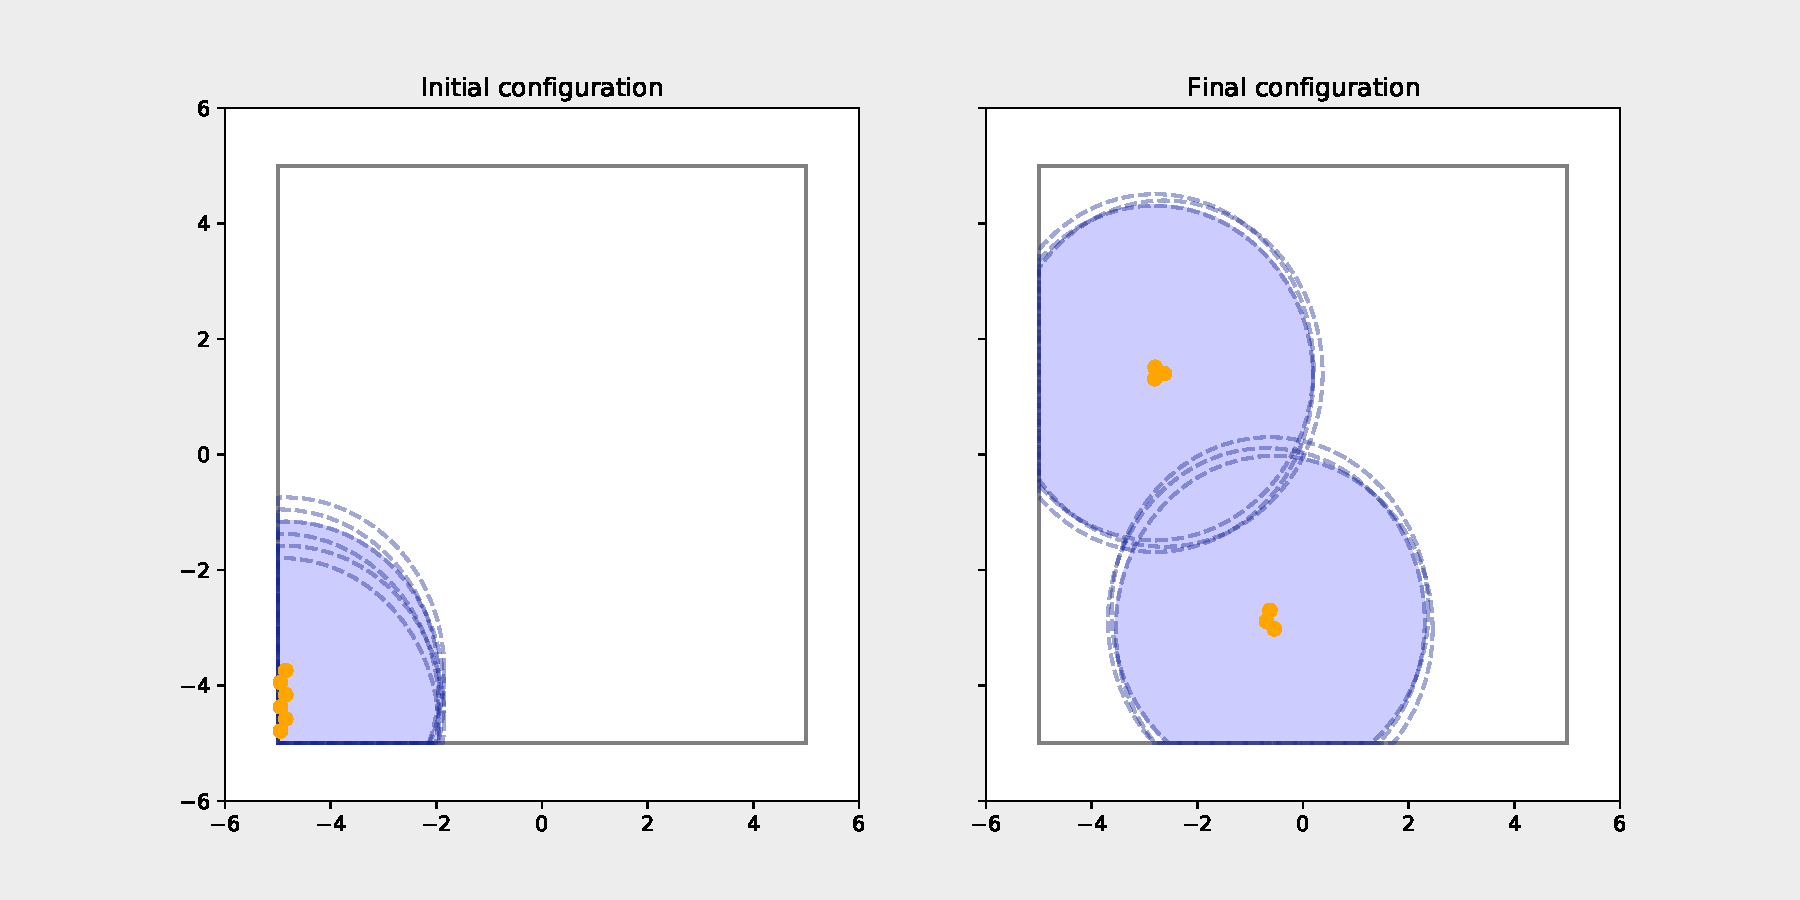
\includegraphics[width=\textwidth]{figs/bigworld_6_agnt_k_1_1_k_2_1_distr.pdf}
  \caption{Initial and final configuration of 6 agents in the Rectworld environment with $k_{1} = k_{2} = 1$ (active dispersion).}
  \label{fig:6_agnt_bw_k_1_1_k_2_1_distr}
\end{figure}
\begin{figure}[H]
  \centering
  \begin{subfigure}[t]{0.5\textwidth}
    \centering
    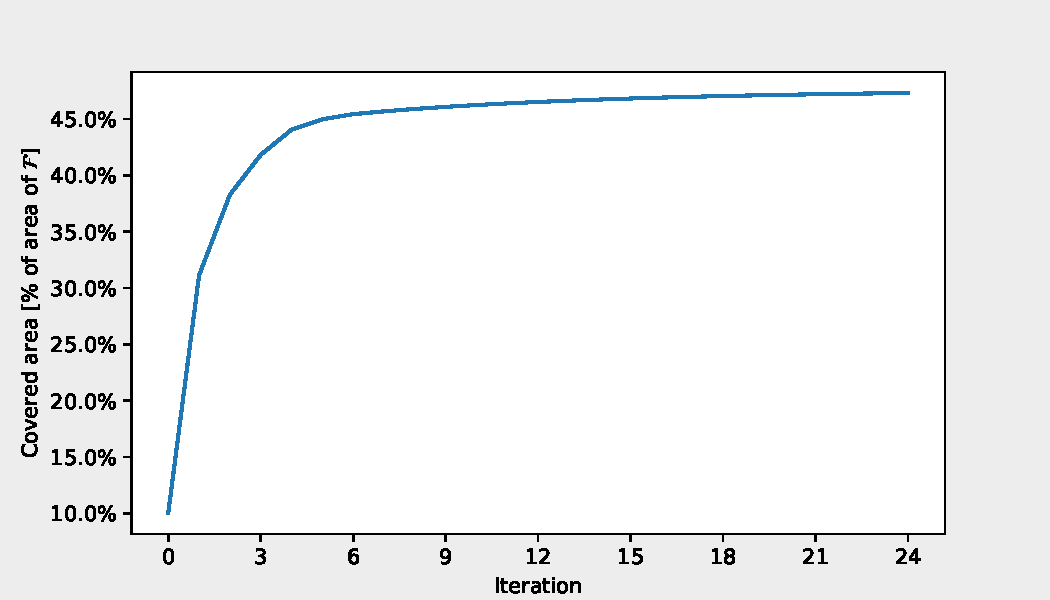
\includegraphics[width=\textwidth]{figs/bigworld_6_agnt_k_1_1_k_2_1_area_traj.pdf}
    \caption{Coverage evolution for 6 agents in the Rectworld environment with $k_{1} = k_{1} = 1$ (active dispersion).}
    \label{fig:6_agnt_bw_k_1_1_a_traj}
  \end{subfigure}%
  ~ 
  \begin{subfigure}[t]{0.5\textwidth}
    \centering
    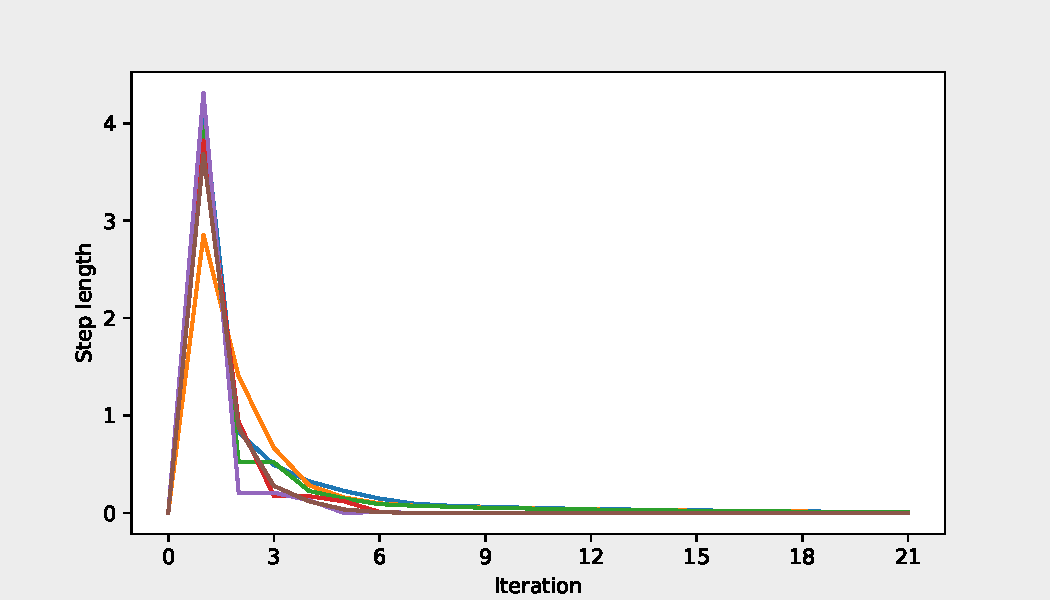
\includegraphics[width=\textwidth]{figs/bigworld_6_agnt_k_1_1_k_2_1_step_traj.pdf}
    \caption{Step length evolution for 6 agents in the Rectworld environment with $k_{1} = k_{1} = 1$ (active dispersion).}
    \label{fig:6_agnt_bw_k_1_1_s_traj}
  \end{subfigure}
  \caption{Coverage percentage and step length evolution for 6 agents in the Rectworld environment when active dispersion is used.}
  \label{fig:6_agnt_bw_evolution_active}
\end{figure}

%%%

\begin{figure}[H]
  \centering
  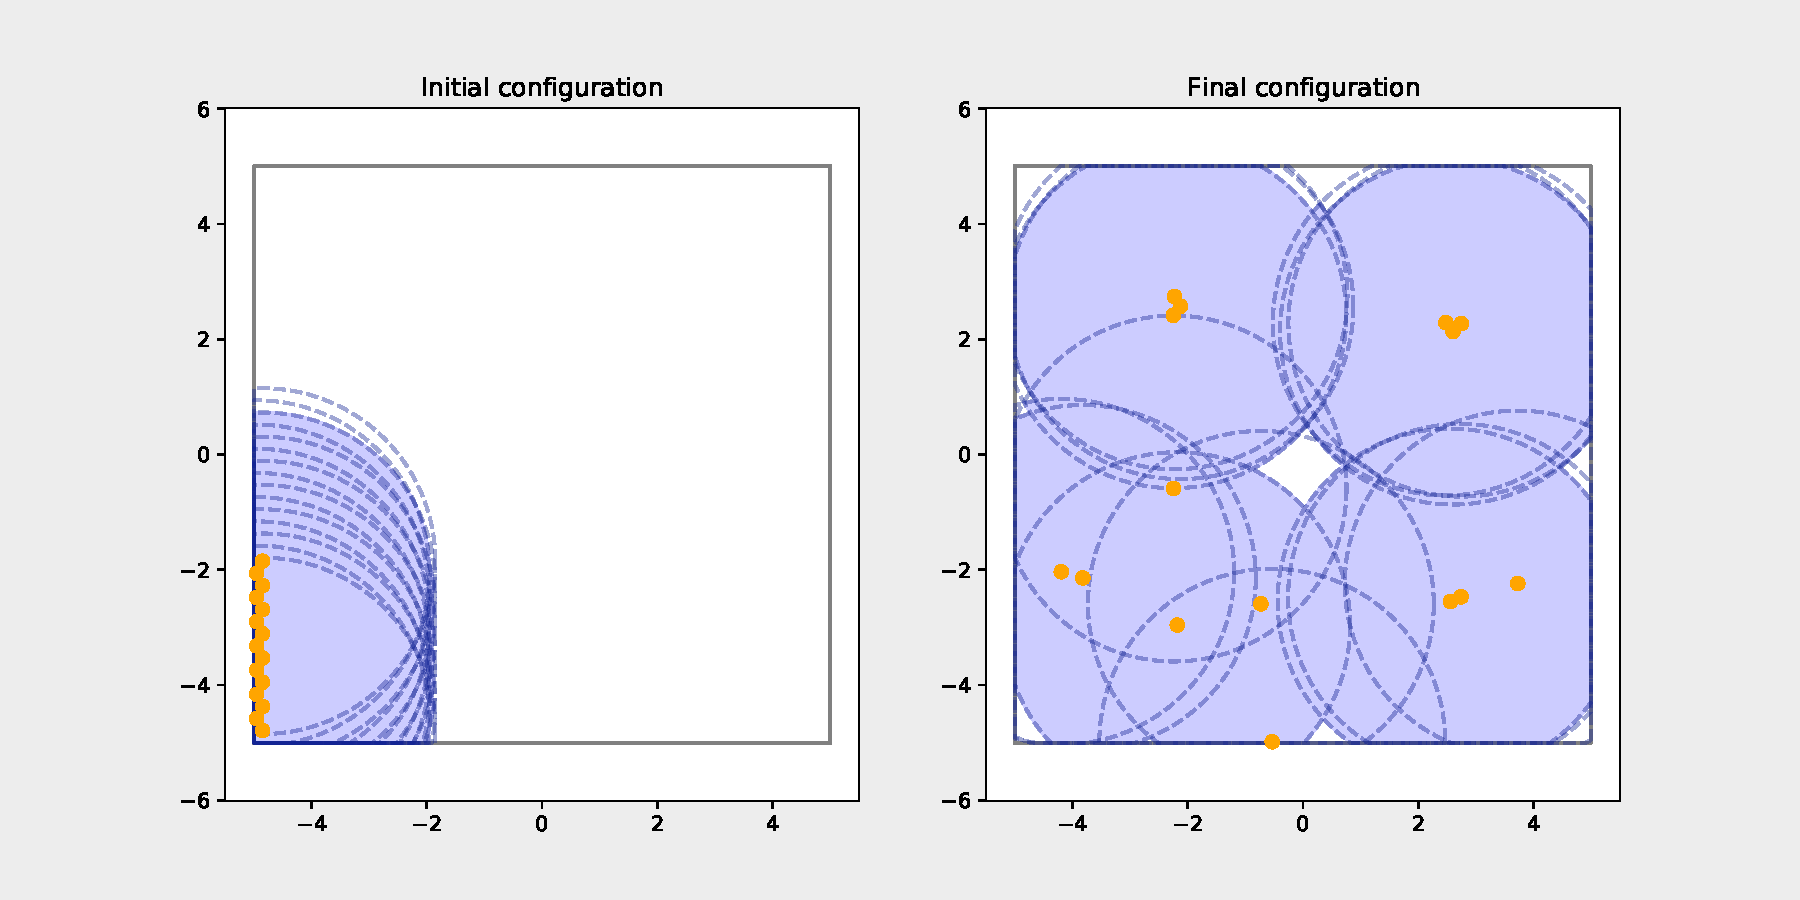
\includegraphics[width=\textwidth]{figs/bigworld_15_agnt_k_1_0_k_2_1_distr.pdf}
  \caption{Initial and final configuration of 15 agents in the Rectworld environment with $k_{1} = 0$ (no active dispersion).}
  \label{fig:15_agnt_bw_k_1_0_k_2_1_distr}
\end{figure}
\begin{figure}[H]
  \centering
  \begin{subfigure}[t]{0.5\textwidth}
    \centering
    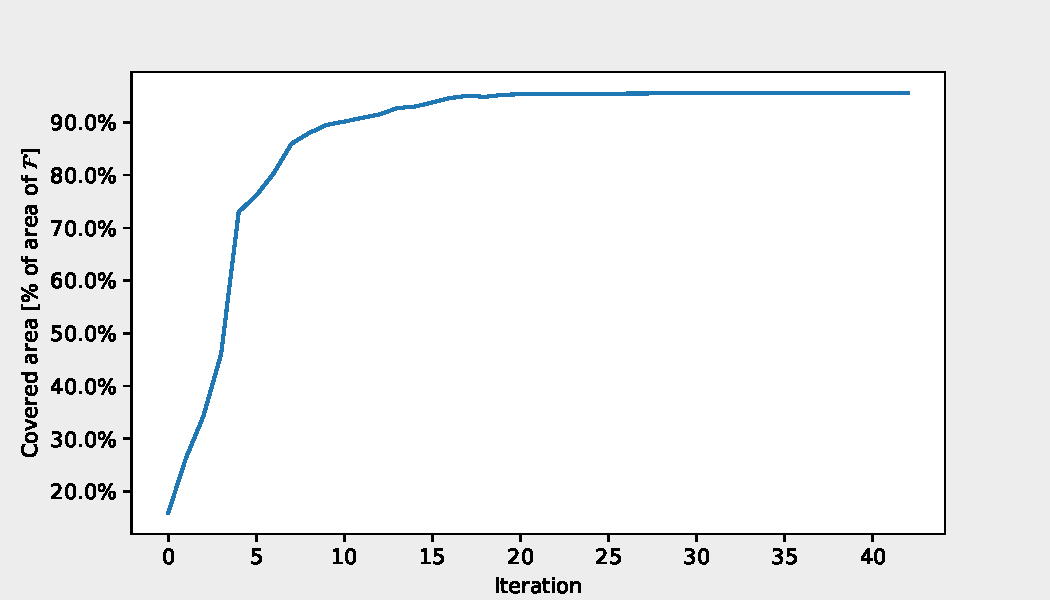
\includegraphics[width=\textwidth]{figs/bigworld_15_agnt_k_1_0_k_2_1_area_traj.pdf}
    \caption{Coverage evolution for 15 agents in the Rectworld environment with $k_{1} = 0$ (no active dispersion).}
    \label{fig:15_agnt_bw_k_1_0_a_traj}
  \end{subfigure}%
  ~ 
  \begin{subfigure}[t]{0.5\textwidth}
    \centering
    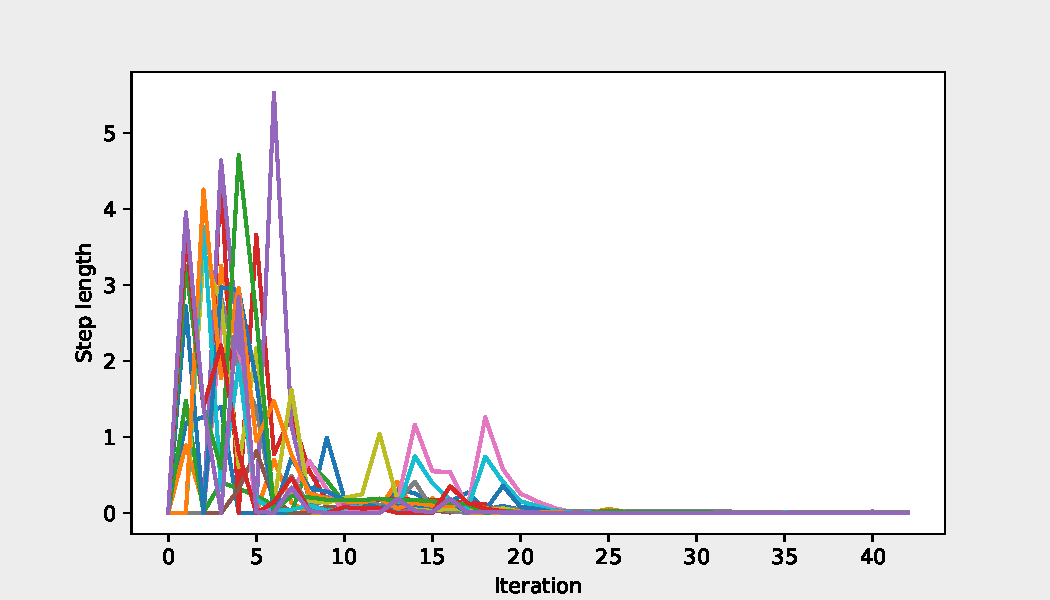
\includegraphics[width=\textwidth]{figs/bigworld_15_agnt_k_1_0_k_2_1_step_traj.pdf}
    \caption{Step length evolution for 15 agents in the Rectworld environment with $k_{1} = 0$ (no active dispersion).}
    \label{fig:15_agnt_bw_k_1_0_s_traj}
  \end{subfigure}
  \caption{Coverage percentage and step length evolution for 15 agents in the Rectworld environment when no active dispersion is used.}
  \label{fig:15_agnt_bw_evolution}
\end{figure}


\begin{figure}[H]
  \centering
  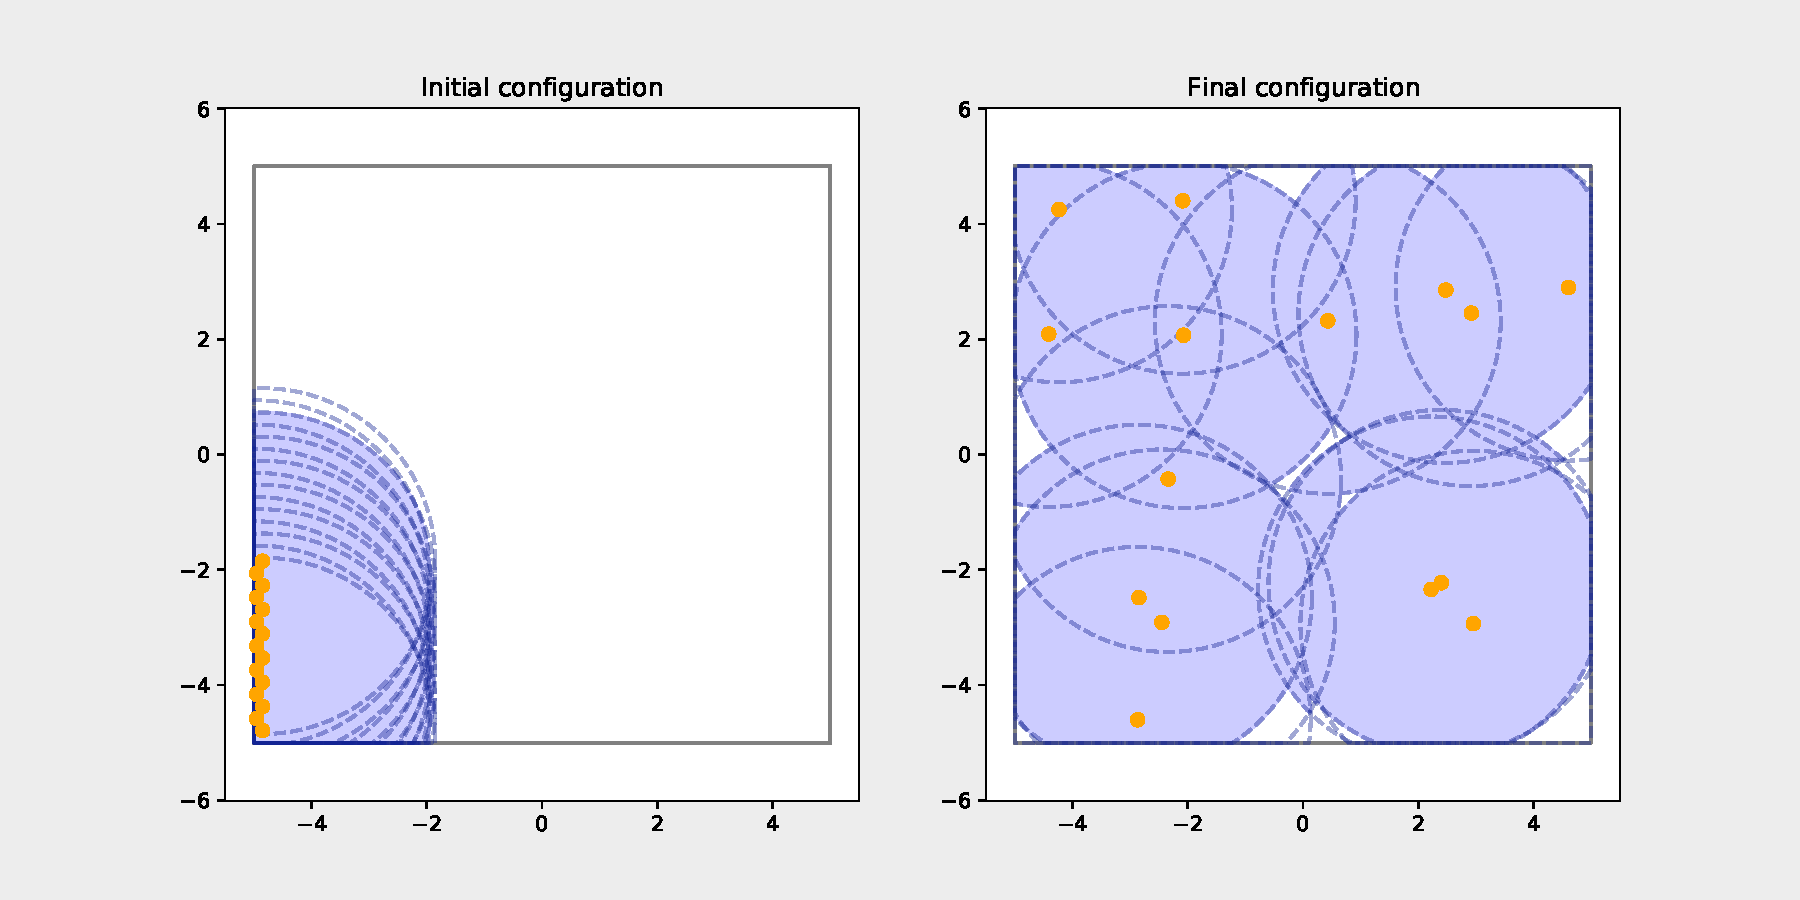
\includegraphics[width=\textwidth]{figs/bigworld_15_agnt_k_1_1_k_2_1_distr.pdf}
  \caption{Initial and final configuration of 15 agents in the Rectworld environment with $k_{1} = k_{2} = 1$ (active dispersion).}
  \label{fig:15_agnt_bw_k_1_1_k_2_1_distr}
\end{figure}
\begin{figure}[H]
  \centering
  \begin{subfigure}[t]{0.5\textwidth}
    \centering
    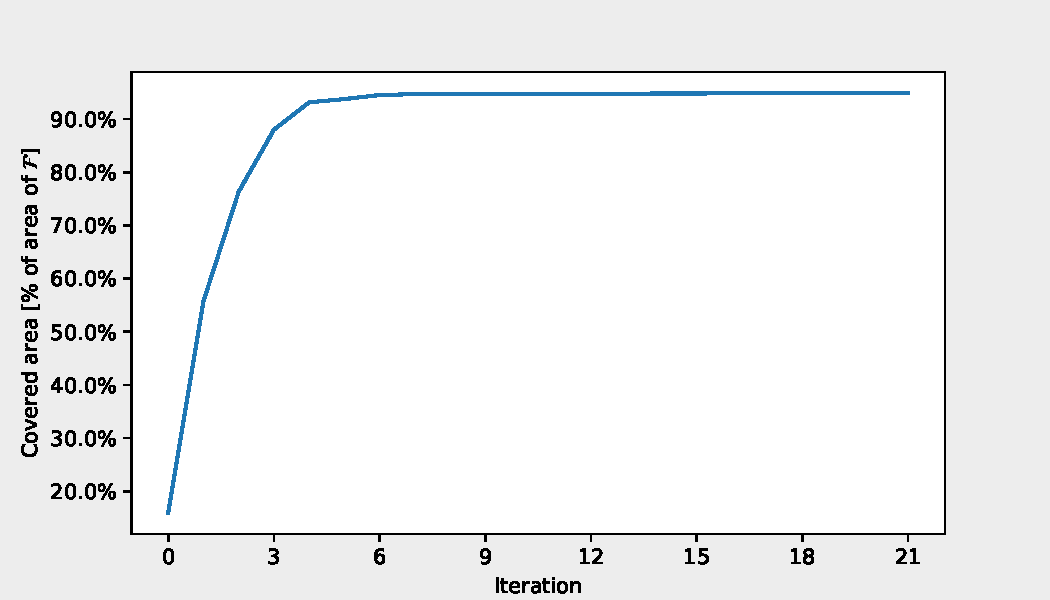
\includegraphics[width=\textwidth]{figs/bigworld_15_agnt_k_1_1_k_2_1_area_traj.pdf}
    \caption{Coverage evolution for 15 agents in the Rectworld environment with $k_{1} = k_{1} = 1$ (active dispersion).}
    \label{fig:15_agnt_bw_k_1_1_a_traj}
  \end{subfigure}%
  ~ 
  \begin{subfigure}[t]{0.5\textwidth}
    \centering
    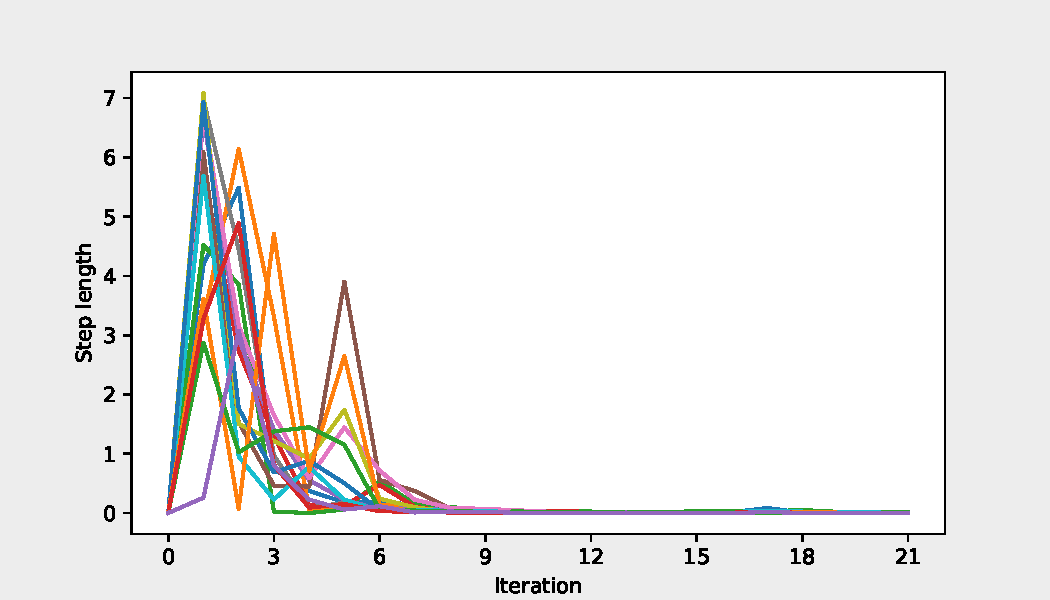
\includegraphics[width=\textwidth]{figs/bigworld_15_agnt_k_1_1_k_2_1_step_traj.pdf}
    \caption{Step length evolution for 15 agents in the Rectworld environment with $k_{1} = k_{1} = 1$ (active dispersion).}
    \label{fig:15_agnt_bw_k_1_1_s_traj}
  \end{subfigure}
  \caption{Coverage percentage and step length evolution for 15 agents in the Rectworld environment when active dispersion is used.}
  \label{fig:15_agnt_bw_evolution_active}
\end{figure}
\clearpage
\subsection{Complexworld}\label[secc]{complexworld}
The Complexworld is constructed to evaluate the performance of Algorithm \ref{alg:alg1} for a large swarm in a larger and more demanding environment.
Simulations are performed with and without active dispersion for a swarm of 50 agents. The results are shown in 
\Crefrange{fig:50_agnt_cw_k_1_0_k_2_1_distr}{fig:50_agnt_tw_evolution_active}.
\begin{figure}[H]
  \centering
  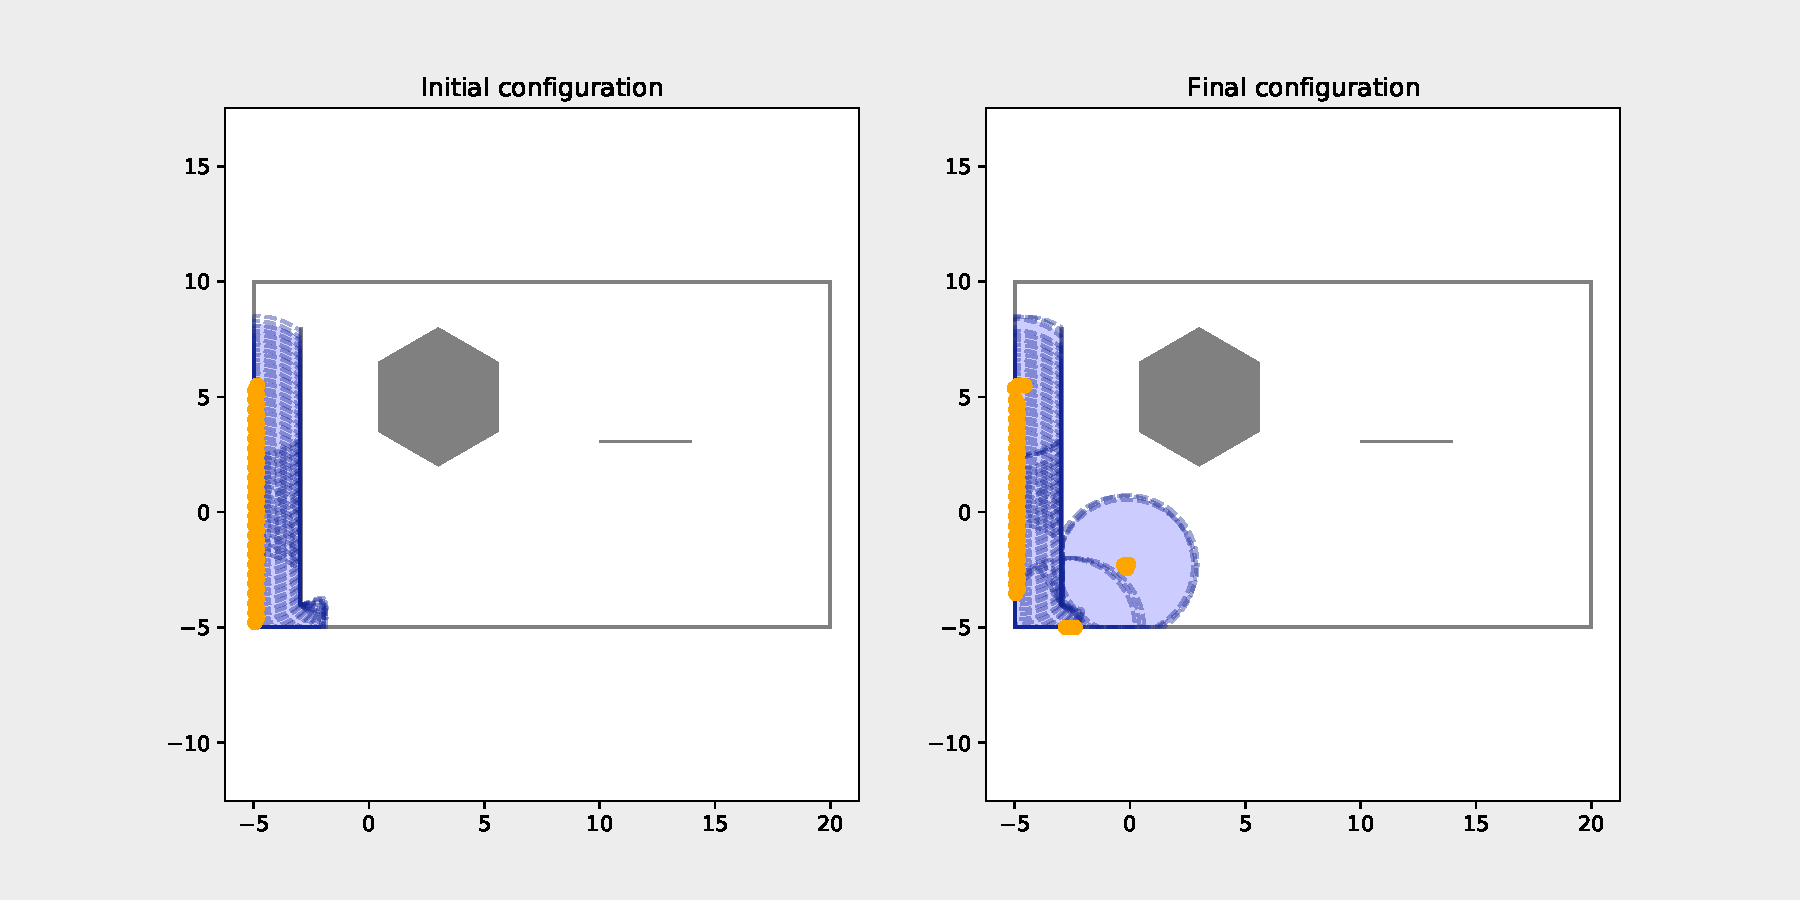
\includegraphics[width=\textwidth]{figs/complexworld_50_agnt_k_1_0_k_2_1_distr.pdf}
  \caption{Initial and final configuration of 50 agents in the Complexworld environment with $k_{1} = k_{2} = 1$ (active dispersion).}
  \label{fig:50_agnt_cw_k_1_0_k_2_1_distr}
\end{figure}

\begin{figure}[H]
  \centering
  \begin{subfigure}[t]{0.5\textwidth}
    \centering
    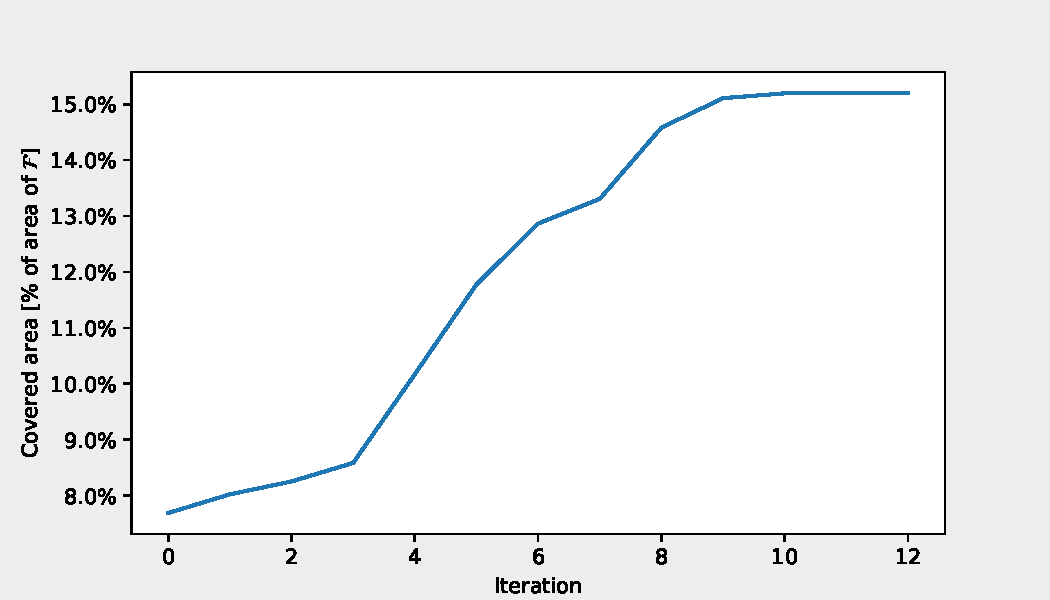
\includegraphics[width=\textwidth]{figs/complexworld_50_agnt_k_1_0_k_2_1_area_traj.pdf}
    \caption{Coverage evolution for 50 agents in the Complexworld environment with $k_{1} = k_{2} = 1$ (active dispersion).}
    \label{fig:50_agnt_cw_k_1_0_k_2_1_a_traj}
  \end{subfigure}%
  ~ 
  \begin{subfigure}[t]{0.5\textwidth}
    \centering
    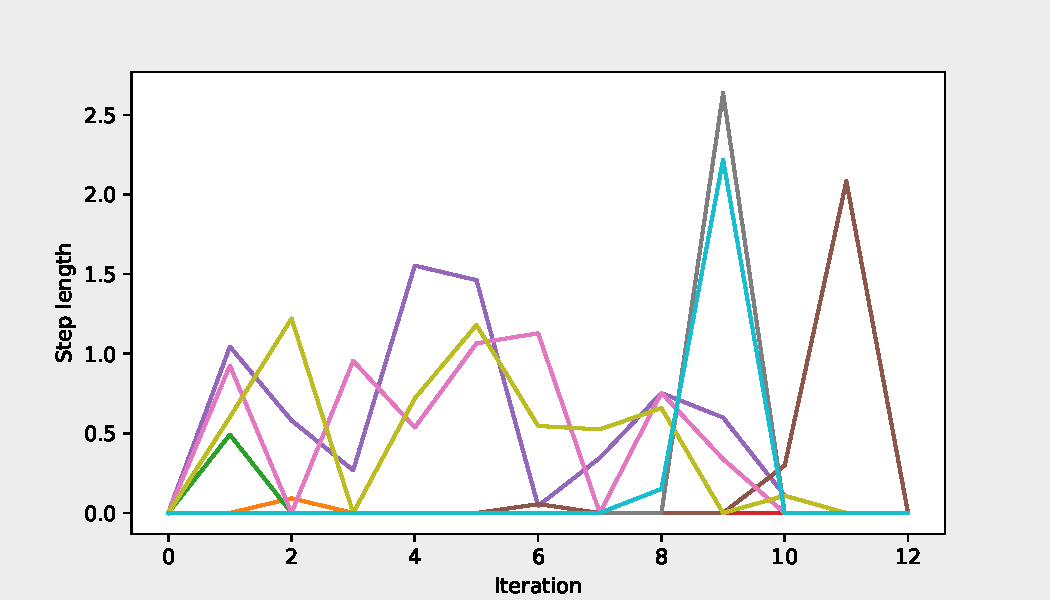
\includegraphics[width=\textwidth]{figs/complexworld_50_agnt_k_1_0_k_2_1_step_traj.pdf}
    \caption{Step length evolution for 50 agents in the Complexworld environment with $k_{1} = k_{2} = 1$ (active dispersion).}
    \label{fig:50_agnt_cw_k_1_0_k_2_1_s_traj}
  \end{subfigure}
  \caption{Coverage percentage and step length evolution for 50 agents in the Complexworld environment when active dispersion is used.}
  \label{fig:50_agnt_cw_evolution}
\end{figure}


\begin{figure}[H]
  \centering
  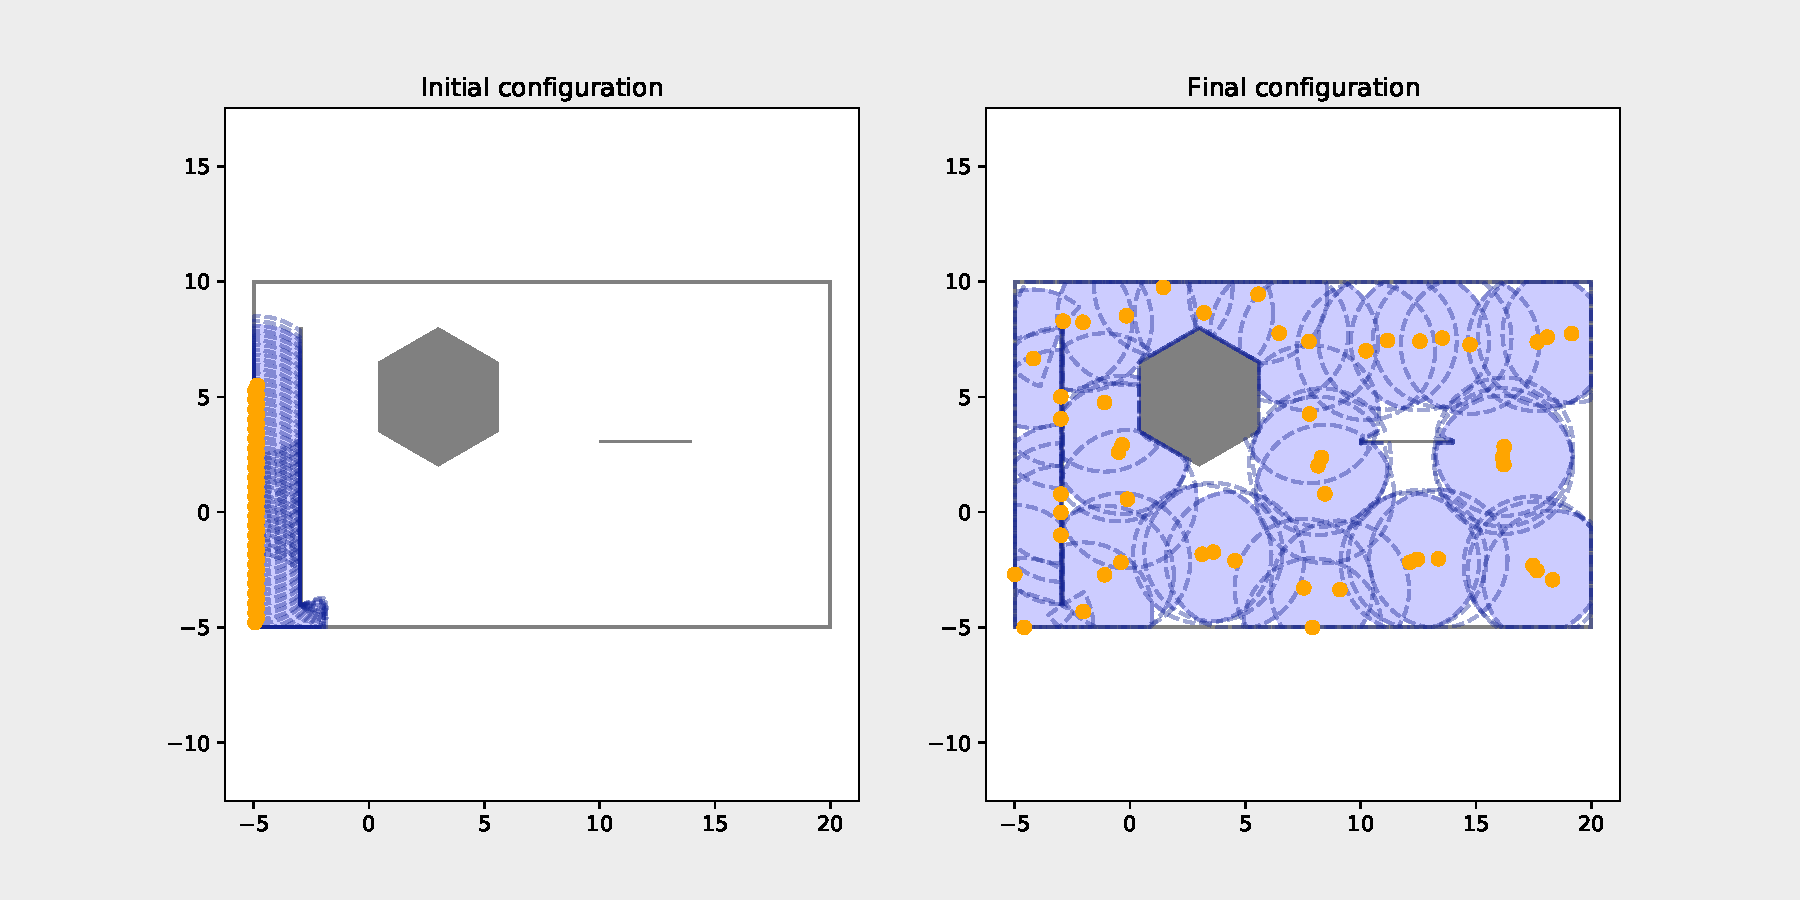
\includegraphics[width=\textwidth]{figs/complexworld_50_agnt_k_1_1_k_2_1_distr.pdf}
  \caption{Initial and final configuration of 50 agents in the Complexworld environment with $k_{1} = k_{2} = 1$ (active dispersion).}
  \label{fig:50_agnt_cw_k_1_1_k_2_1_distr}
\end{figure}

\begin{figure}[H]
  \centering
  \begin{subfigure}[t]{0.5\textwidth}
    \centering
    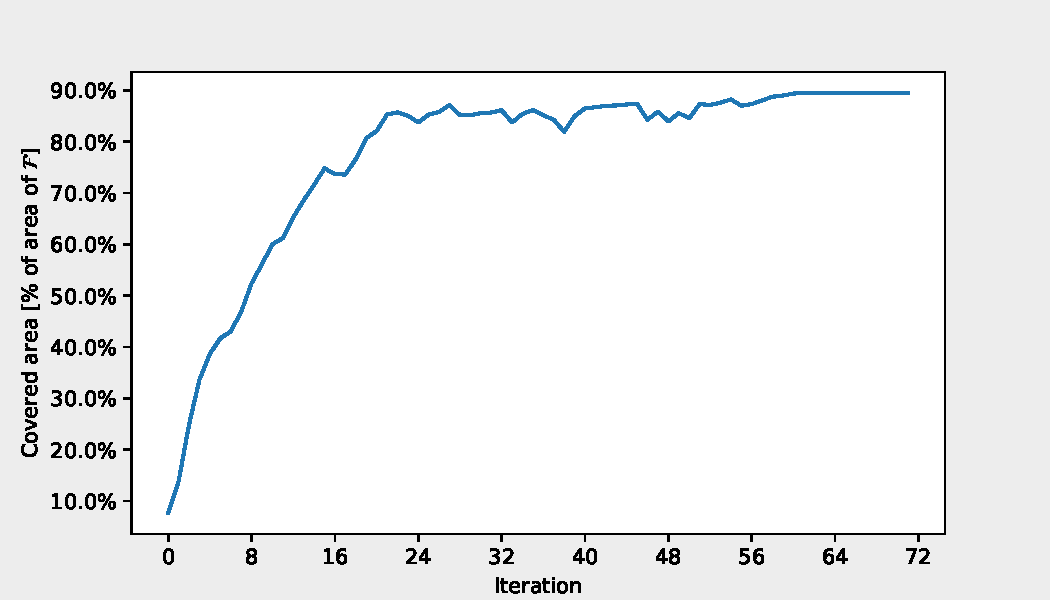
\includegraphics[width=\textwidth]{figs/complexworld_50_agnt_k_1_1_k_2_1_area_traj.pdf}
    \caption{Coverage evolution for 50 agents in the Complexworld environment with $k_{1} = k_{2} = 1$ (active dispersion).}
    \label{fig:50_agnt_cw_k_1_k_2_1_a_traj}
  \end{subfigure}%
  ~ 
  \begin{subfigure}[t]{0.5\textwidth}
    \centering
    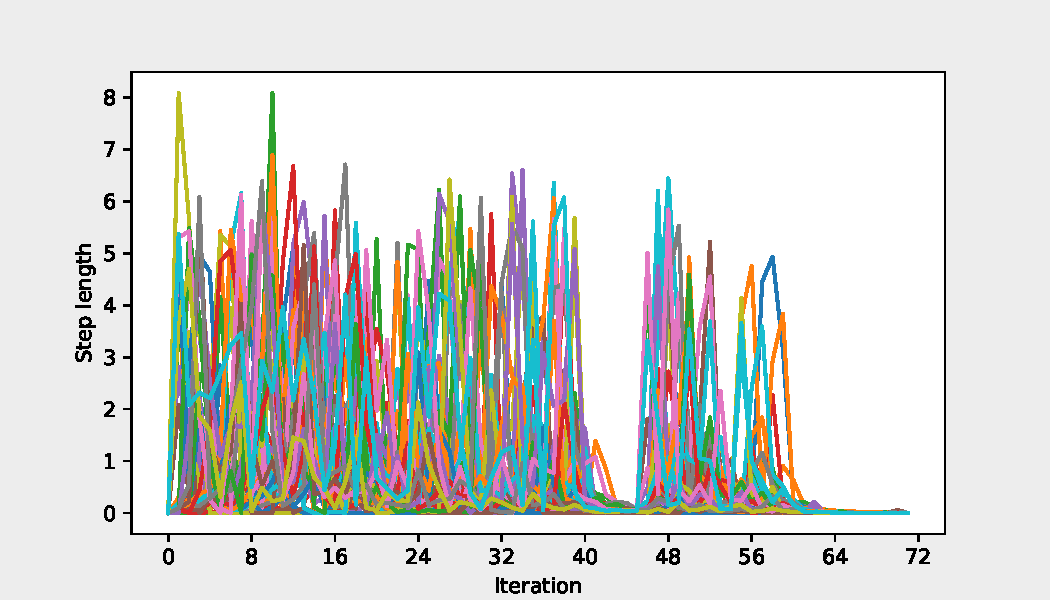
\includegraphics[width=\textwidth]{figs/complexworld_50_agnt_k_1_1_k_2_1_step_traj.pdf}
    \caption{Step length evolution for 50 agents in the Complexworld environment with $k_{1} = k_{2} = 1$ (active dispersion).}
    \label{fig:50_agnt_cw_k_1_1_k_2_1_s_traj}
  \end{subfigure}
  \caption{Coverage percentage and step length evolution for 50 agents in the Complexworld environment when active dispersion is used.}
  \label{fig:50_agnt_tw_evolution_active}
\end{figure}

\section{Discussion}
The results obtained in Section \ref{results} are summarized in Table \ref{tab:sim_res_worlds} and \ref{tab:sim_res_worlds_active}.
\begin{center}
  \captionof{table}{Simulation results for all environments without active dispersion\label{tab:sim_res_worlds}}
  \begin{tabular}{l|l|l|l|l}
    Environment & 3 agents & 6 agents & 15 agents & 50 agents\\
    \hline
    Tinyworld & 100\% & - & - & - \\ 
    Tinyworld2 & 71.8\% & 98\% & - & - \\
    Rectworld &  22.1\% & 24.5\% & 95\% & - \\
    Complexworld & - & - & - & 15.5\% \\
  \end{tabular}
\end{center}
\begin{center}
  \captionof{table}{Simulation results for all environments with active dispersion\label{tab:sim_res_worlds_active}}
  \begin{tabular}{l|l|l|l|l}
    Environment & 3 agents & 6 agents & 15 agents & 50 agents\\
    \hline
    Tinyworld & 100\% & - & - & - \\ 
    Tinyworld2 & 45.2\% & 100\% & - & - \\
    Rectworld &  25\% & 46\% & 93\% & - \\
    Complexworld & - & - & - & 89\% \\
  \end{tabular}
\end{center}

\subsection{Clustering}
In all simulations we see a tendency for agents to gather in groups of three, and cluster as closely together as the constraints \eqref{min_dist_neigh}-\eqref{non_linear_neighb} allow.  
This behavior is especially prevalent when there are not enough agents to cover the entire feasible space, and when active dispersion is not applied. This is due to 
the fact that the intersection of three circles is largest in area when the circle centers coincide. Considering the results in \cite{CRB_multilat} such behavior is disadvantageous. The region in which
the accuracy of multilateration (in presence of measurement noise) is the greatest lies in and around the convex hull of the agents. Tight clustering yields a small convex hull, 
meaning the region in which accurate multilateration can be performed is small.


\subsection{Active dispersion as cluster prevention}
In the Tinyworld environment, whose simulation results are shown in \ref{tinyworld}, we clearly see the effect of active dispersion (\figref{fig:3_agnt_tw_k_1_0_distr} and \figref{fig:3_agnt_tw_k_1_1_k_2_1_distr}). 
In the case where no active dispersion is used the objective function is constant over the feasible space. Hence the initial configuration is one of 
infinitely many equal valued optima, and Algorithm \ref{alg:alg1} halts after one iteration. In the case where active dispersion is applied the agents spread to the corners of the
feasible space as seen in \figref{fig:3_agnt_tw_k_1_1_k_2_1_distr}. This is due to the fact that the local probability of coverage is constant over the feasible space for all agents, hence the 
local optimization problem \eqref{local_opt_prob} is equivalent to maximizing dispersion between an agent $a$ and its neighbors. 

Simulations performed in the Rectworld environment for 15 agents exhibit some of the same behavior. The final configuration obtained when active dispersion
is applied is shown in \figref{fig:15_agnt_bw_k_1_1_k_2_1_distr}. Comparing this to the configuration obtained in the same environment with the same number of agents (see \figref{fig:15_agnt_bw_k_1_0_k_2_1_distr})
we clearly see that the agents are more evenly spread out in the mission space when active dispersion is used. In densely populated areas the gradient of the local probability of coverage tends be small. This is due to the fact that in densely populated areas, 
the majority of the area is covered independently of an agent $a$ covering it or not. Thus any small perturbation of an agents position does not have a major impact on
the agents local probability of coverage. As the number of neighbors for an agent in a densely populated area is large, the dispersion term is significantly negative and has a steep gradient.
This combination of movement having a small impact on the local probability of coverage, and a large impact on the value of the dispersion term causes agents to move away from densely populated areas, 
preventing clustering.

Active dispersion does however not prevent clustering in sparsely populated areas. This can be seen by the configurations for 3 and 6 agents in the
Rectworld environment (\ref{fig:3_agnt_bw_k_1_1_k_2_1_distr} and \ref{fig:6_agnt_bw_k_1_1_k_2_1_distr}). In these configurations any
movement from the current configuration would cause the local
probability of coverage for the agent that moves to drop significantly. Furthermore none of the agents have enough neighbors to force them to move despite
the drop in local probability of coverage.

\subsection{Effect of improperly weighted active dispersion}
The simulations performed for a swarm of size 3 in the Tinyworld2 environment display a weakness of active dispersion. Here the swarm covers a significantly smaller percentage of the 
feasible space when applying active dispersion than when not. This is due to the fact that the dispersion term is weighted to heavily. When the local probability of coverage for an agent is small, i.e. $L(\mathbf{X}_{\mathcal{B}_{a}\cup\{a\}})$ is small 
for all possible values of $\mathbf{x}_{a}$, the value of 
the local objective \eqref{totally_objective} is dominated by the dispersion term. This causes a shift in behavior. The focus is on dispersion rather than coverage, and Algorithm \ref{alg:alg1} converges
to a solution that gives a smaller percentage of covered area.

For a swarm of 6 agents in the Tinyworld2 environment the case is quite different. Now active dispersion yields a configuration that gives a larger coverage percentage than when no active
dispersion is applied. This result is although not a consequence of clever objective function formulation. As for three agents the active dispersion term dominates the coverage term
in \eqref{totally_objective} due to local probability of coverage being small no matter the value of $\mathbf{x}_{a}$. Hence the agents focus on maximizing dispersion rather than covered area. The 
solution generated by Algorithm \ref{alg:alg1} for 6 agents in the Tinyworld2 environment is identical to the solution generated for 6 agents in the Tinyworld environment when applying active dispersion. 
This makes it obvious that the high percentage of coverage obtained in the Tinyworld2 environment using active dispersion is not caused by the agents meticulously positioning themselves as to maximize the local
probability of coverage. Instead they position themselves so that the maximum dispersion is obtained, and the higher percentage of coverage is simply a lucky bi-effect.


\subsection{Active dispersion forcing exploration}

\figref{fig:6_agnt_bw_k_1_0_k_2_1_distr} shows the configuration obtained
by running Algorithm \ref{alg:alg1} for a swarm of size 6 in the Rectworld environment  without active dispersion. Here we see that the three agents in the bottom-left corner stay
at their initial positions throughout the simulation, and that the bottom left corner is covered by all 6 agents. As the minimum requirement for coverage is three agents, the swarm could 
clearly be utilized to give a higher percentage of coverage. \figref{fig:bw_x_traj} shows the configuration of the swarm after each iteration of Algorithm \ref{alg:alg1}. It is clear that 
throughout the iterations the visible sets of the bottom three agents are covered by those of the top three agents. Thus the local objective value for the bottom three agents is zero 
throughout the iterations, and any infinitesimal perturbation of their positions cause no change to the objective value, i.e. zero gradient. The SQP solver concludes that the bottom three agents are at local
optima at each iteration, and no change is made to their position. 

The configuration generated for a swarm of size 6 using active dispersion in the Rectworld environment (see \figref{fig:6_agnt_bw_k_1_1_k_2_1_distr}) does not exhibit the same behavior as the aforementioned configuration. This can be attributed to the
larger initial step sizes due to active dispersion (see \ref{fig:6_agnt_bw_k_1_0_s_traj} and \ref{fig:6_agnt_bw_k_1_1_s_traj}) causing no agents to have their entire visible set covered by those of three or more other agents.
Thus no agent is left with a constant-zero local probability of coverage, and the swarm reaches a higher percentage of coverage.

\begin{figure}[H]
  \centering
  \includegraphics[width=\textwidth]{figs/bigworld_6_agnt_k_1_0_k_2_1_x_traj.pdf}
  \caption{Intermediate configurations for 6 agents in the Rectworld environment with $k_{1} = 0$ (no active dispersion).}
  \label{fig:bw_x_traj}
\end{figure}

Simulations performed in the Complexworld environment yet again show how active dispersion force agents to explore the mission space. Without active dispersion Algorithm \ref{alg:alg1} converges quickly to a clearly sub-optimal
configuration, as seen in \figref{fig:50_agnt_cw_k_1_0_k_2_1_distr}. Only a small portion of the swarm make advancements into the mission space. Yet again this is caused by the majority of agents having a zero-gradient
local objective in every iteration of Algorithm \ref{alg:alg1} due to their visible sets being fully contained by those of at least three other agents. With active dispersion applied agents are explicitly encouraged to explore. Thus, as seen in \figref{fig:50_agnt_cw_k_1_1_k_2_1_distr}, agents disperse into the mission space and 
reach a far higher percentage of coverage than earlier. 

\subsection{Local convergence causing sub-optimal configurations}
For a swarm of 3 agents in the Rectworld environment the final configurations obtained with 
and without active dispersion are shown in 
\ref{fig:3_agnt_bw_k_1_1_k_2_1_distr} and \ref{fig:3_agnt_bw_k_1_0_k_2_1_distr} respectively. It is clear that the two configurations do not differ much, except that the configuration obtained when using active dispersion
is translated slightly to the north-east. As shown in \figref{fig:3_agnt_bw_k_1_0_s_traj} and \figref{fig:3_agnt_bw_k_1_1_s_traj} the agents make larger initial steps when active dispersion is applied. This
causes them to move further into the mission space. Thus less of their visual sets are clipped by the walls of the mission space, resulting in a larger percentage of covered area.

Both configurations obtained for 3 agents in the Rectworld environment exhibit the same problematic behavior. Moving the entire swarm in the north-east direction would yield higher percentage of covered area,
but Algorithm \ref{alg:alg1} converges with the swarm placed so that the area covered by the three agents is clipped by the mission space walls. This is due to Algorithm \ref{alg:alg1} optimizing
the configuration of the swarm one agent at the time. In order to move the entire swarm to the north-east direction, all agents would have to move in the north east direction, and they
would have to do so one at the time. In the configuration shown in \figref{fig:3_agnt_bw_k_1_0_k_2_1_distr} no single agent would increase their local objective by moving, although they would all benefit from each other moving.
Due to no single agent benefiting from moving Algorithm \ref{alg:alg1} converges to a clearly sub-optimal configuration.

\figref{fig:6_agnt_bw_k_1_1_k_2_1_distr} shows the final configuration obtained for a swarm of 6 agents in the Rectworld environment using active dispersion. Again translating the
entire swarm north-east would give a higher percentage of coverage, but due to all agents being at local optima of their local objective functions, Algorithm \ref{alg:alg1} halts, and yields
a clearly sub-optimal configuration.
\section{Future Work}
\bibliographystyle{IEEEtran}
\bibliography{bibliography.bib}

\end{document}
